\label{results}
\subsection{Comparing the three D meson correlation distributions}
To check the compatibility of three D meson analyses, Figure ~\ref{fig:DataD0DpDs} shows the corrected azimuthal correlation distributions (except for the feed-down subtraction and the secondary contamination removal) for $\Dzero$-h, $\Dstar$-h and $\Dplus$-h, in each column, on the data sample used in the analysis. Results are shown for $3 < D\ p_\text{T} < 5$ GeV/$c$, $5 < D\ p_\text{T} < 8$ GeV/$c$, $8 < D \ p_\text{T} < 16$ GeV/$c$ and $16 < D\ p_\text{T} < 24$ GeV/$c$ with associated tracks $p_\text{T} > 0.3$, $p_\text{T} > 1$, $0.3 < p_\text{T} < 1$ GeV/$c$, $1 < p_\text{T} < 2$ GeV/$c$, $2 < p_\text{T} < 3$ GeV/$c$ and $ p_\text{T} > 3$ GeV/$c$.

\begin{figure}[htbp]
\centering
% 2-3 GeV/c
{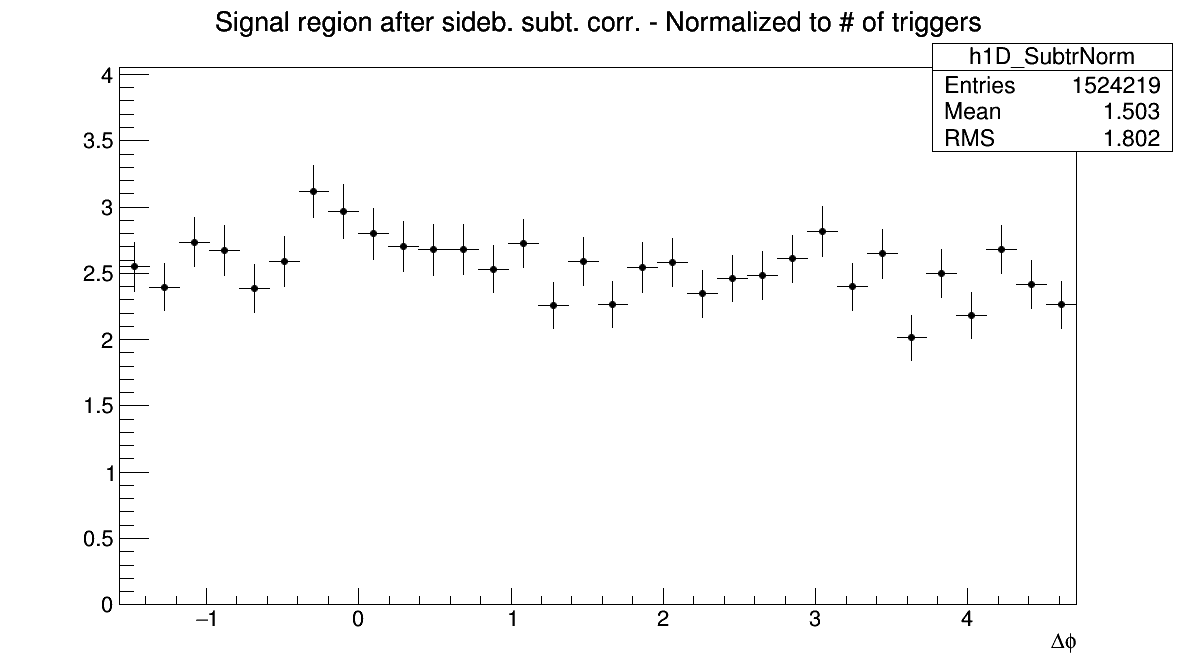
\includegraphics[width=0.31\linewidth, height=0.23\linewidth]{figures/DplusPlotsweff/AzimCorrDistr_Dplus_Canvas_PtIntBins2to2_PoolInt_thrdot3to99dot.png}}
{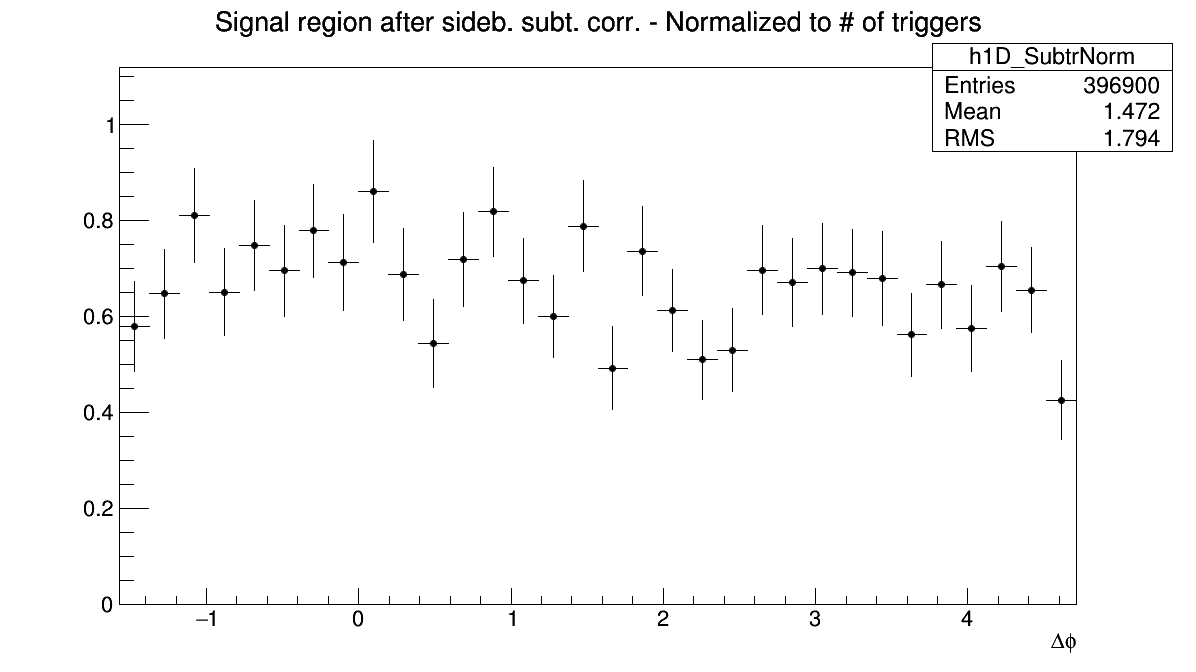
\includegraphics[width=0.31\linewidth, height=0.23\linewidth]{figures/DplusPlotsweff/AzimCorrDistr_Dplus_Canvas_PtIntBins2to2_PoolInt_thr1dotto99dot.png}}
{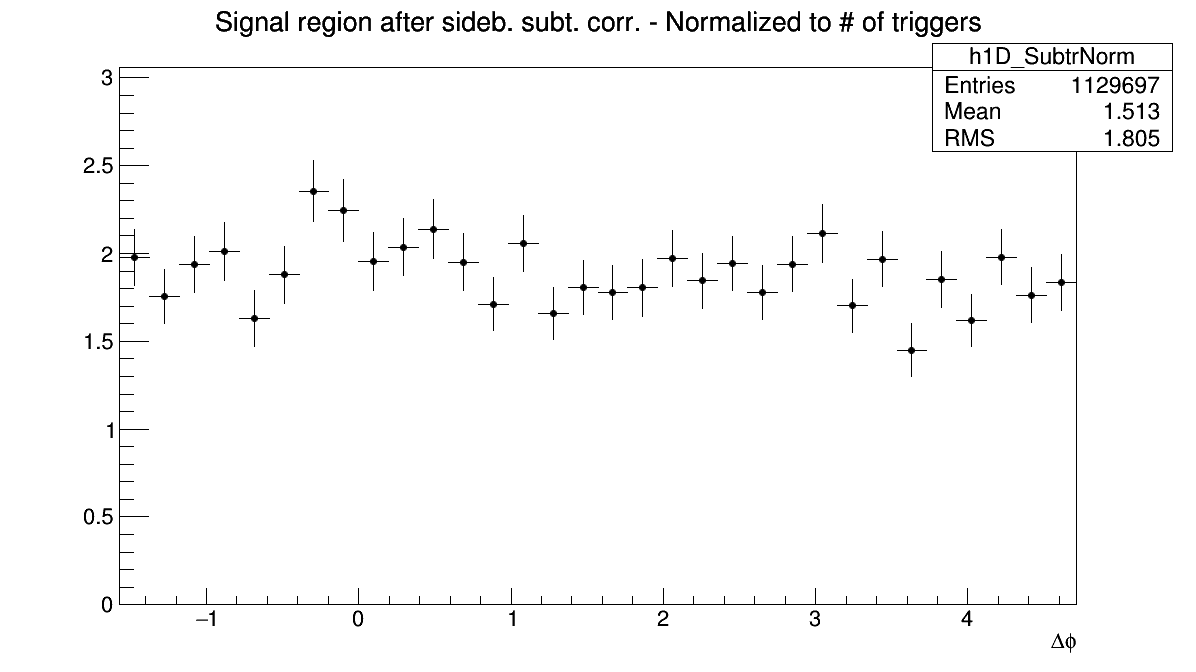
\includegraphics[width=0.31\linewidth, height=0.23\linewidth]{figures/DplusPlotsweff/AzimCorrDistr_Dplus_Canvas_PtIntBins2to2_PoolInt_thrdot3to1dot.png}}
{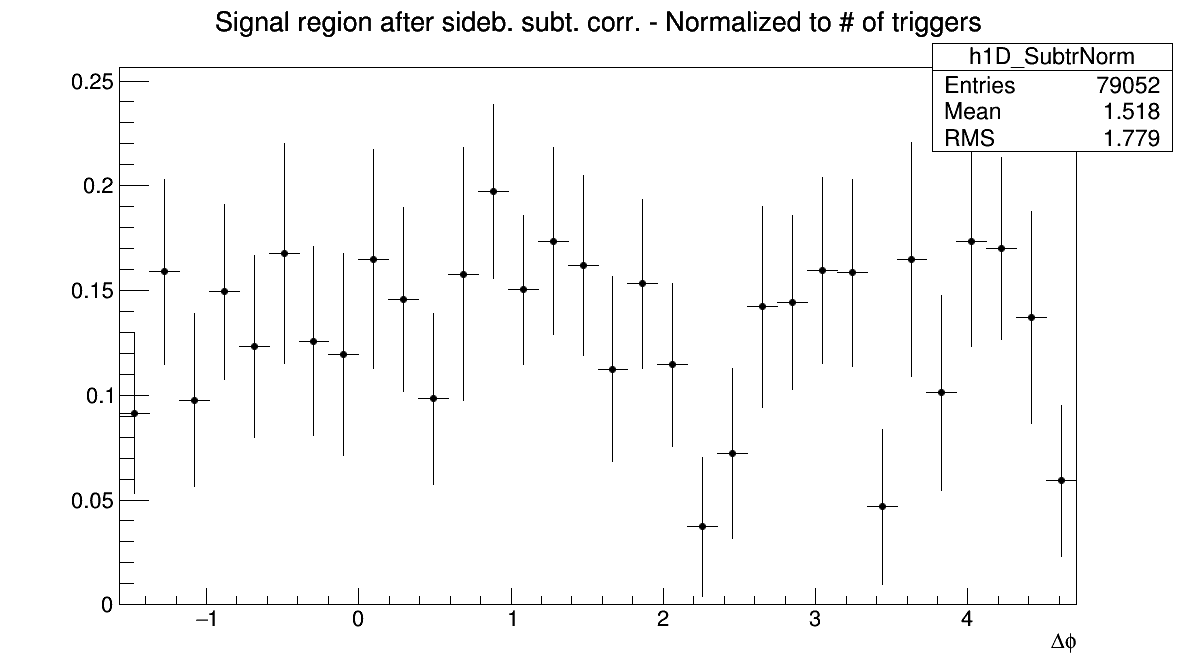
\includegraphics[width=0.31\linewidth, height=0.23\linewidth]{figures/DplusPlotsweff/AzimCorrDistr_Dplus_Canvas_PtIntBins2to2_PoolInt_thr2dotto99dot.png}}
{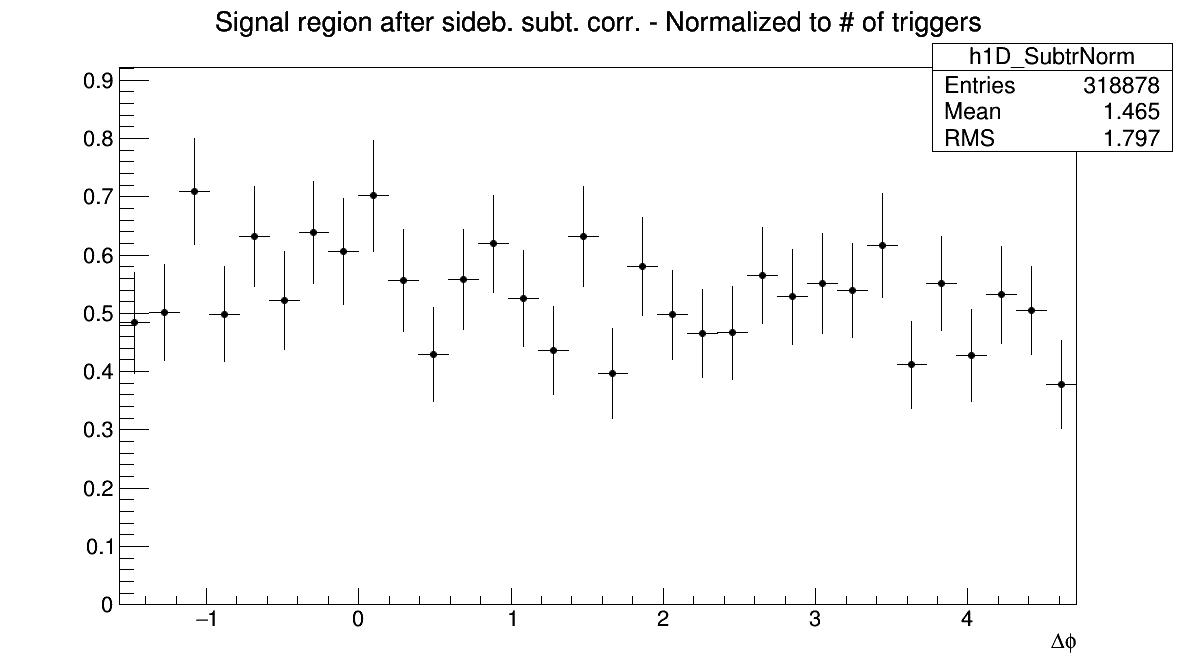
\includegraphics[width=0.31\linewidth, height=0.23\linewidth]{figures/DplusPlotsweff/AzimCorrDistr_Dplus_Canvas_PtIntBins2to2_PoolInt_thr1dotto2dot.png}}
{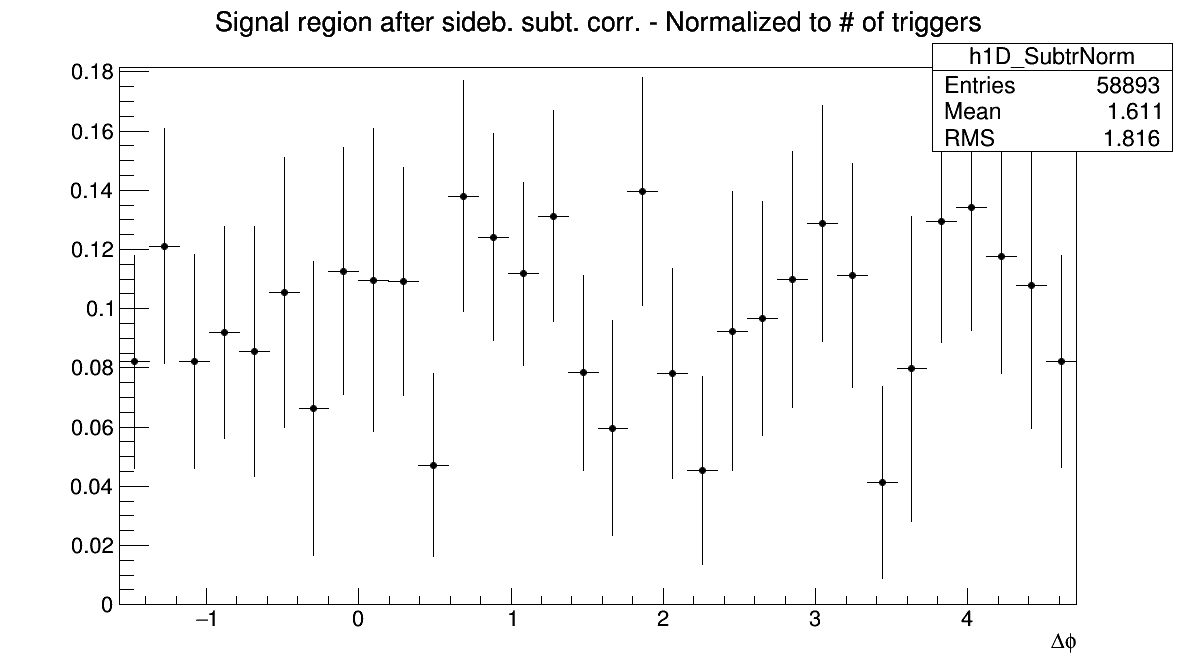
\includegraphics[width=0.31\linewidth, height=0.23\linewidth]{figures/DplusPlotsweff/AzimCorrDistr_Dplus_Canvas_PtIntBins2to2_PoolInt_thr2dotto3dot.png}}

%{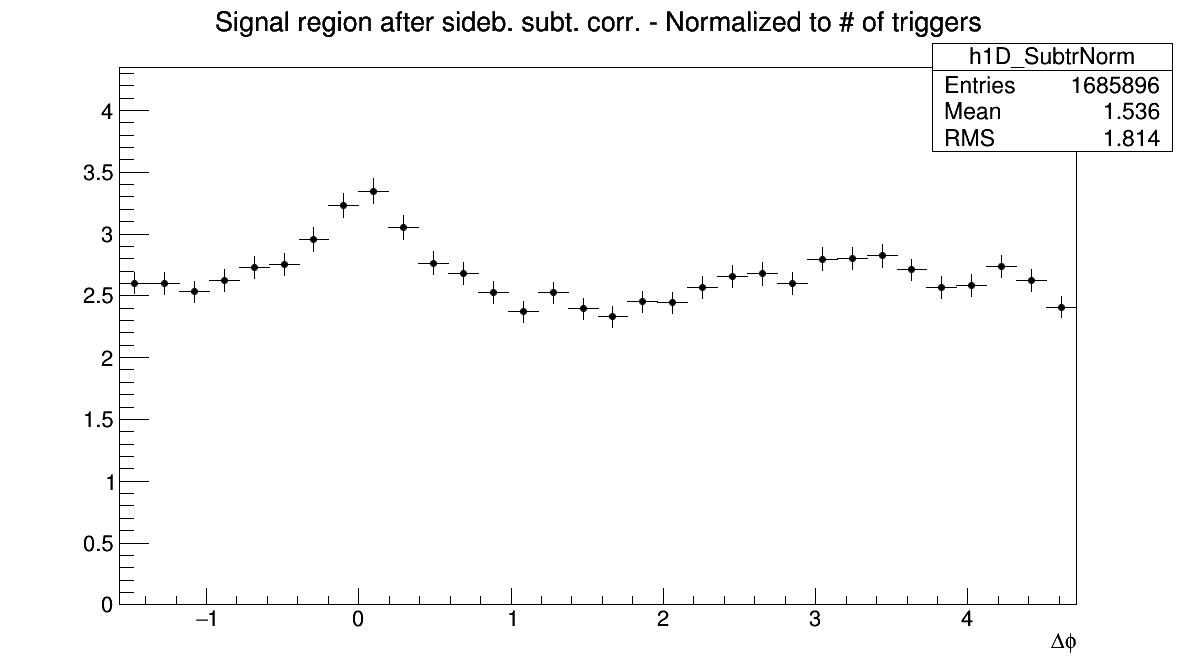
\includegraphics[width=0.33\linewidth, height=0.25\linewidth]
{\includegraphics[width=0.31\linewidth, height=0.23\linewidth]
{figures/Dzero/AzimCorrDistr_Dzero_Canvas_PtIntBins4to5_PoolInt_thrdot3to99dot.png}}
{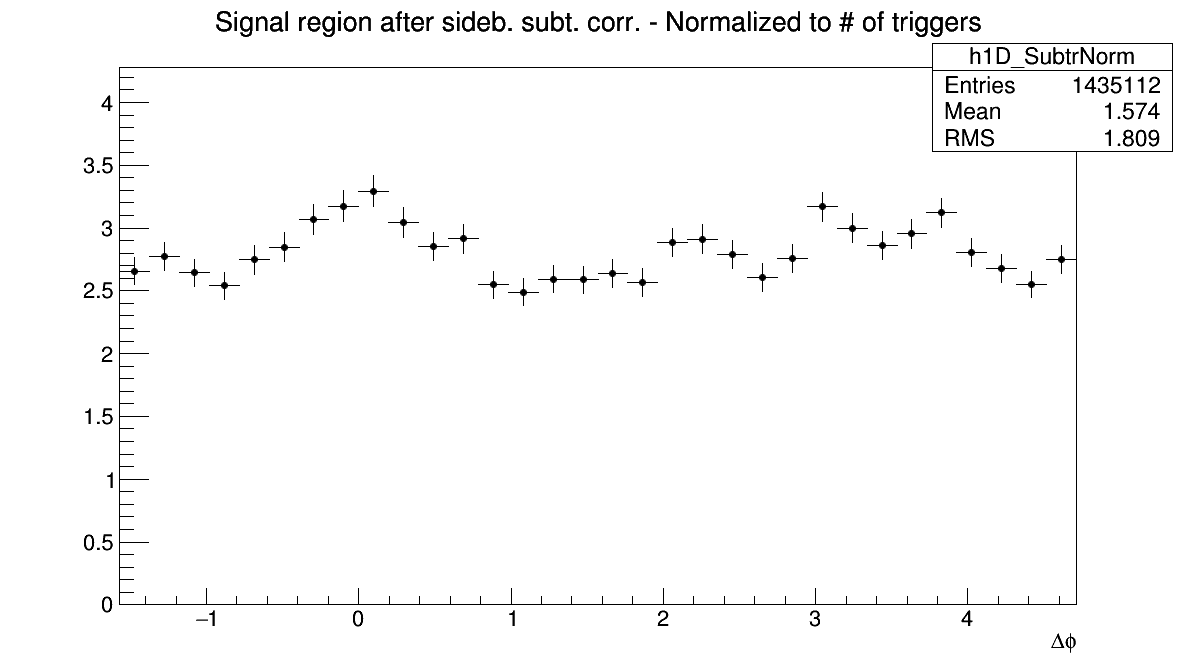
\includegraphics[width=0.31\linewidth, height=0.23\linewidth]{figures/DplusPlotsweff/AzimCorrDistr_Dplus_Canvas_PtIntBins3to4_PoolInt_thrdot3to99dot.png}}
{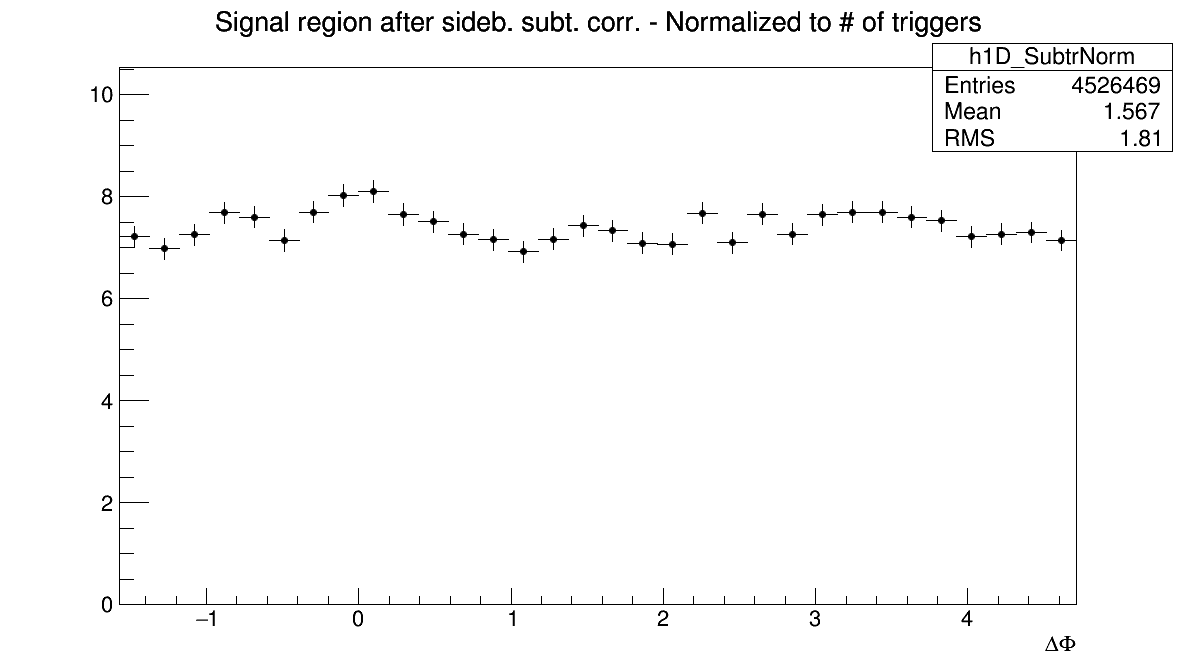
\includegraphics[width=0.31\linewidth, height=0.23\linewidth]{figures/Dstar_wEFF/AzimCorrDistr_Dstar_Canvas_PtIntBins2to3_PoolInt_thrdot3to99dot.png}}
%Pt>1.0GeV/c (LowPt)
{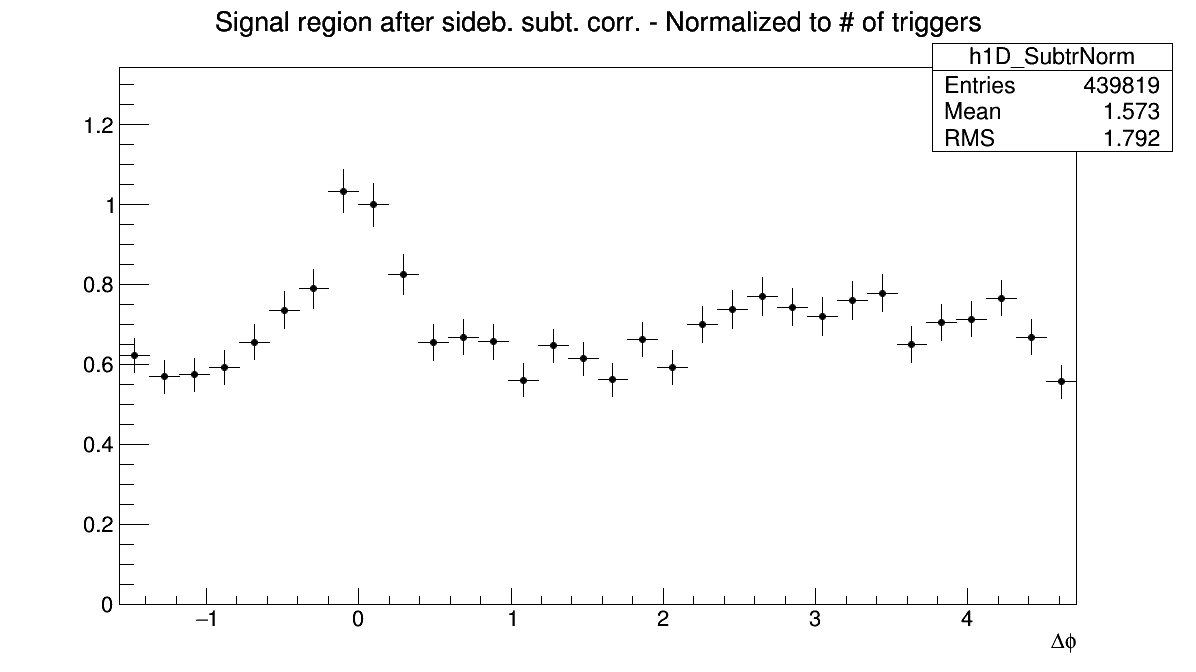
\includegraphics[width=0.31\linewidth, height=0.23\linewidth]{figures/Dzero/AzimCorrDistr_Dzero_Canvas_PtIntBins4to5_PoolInt_thr1dotto99dot.png}}
{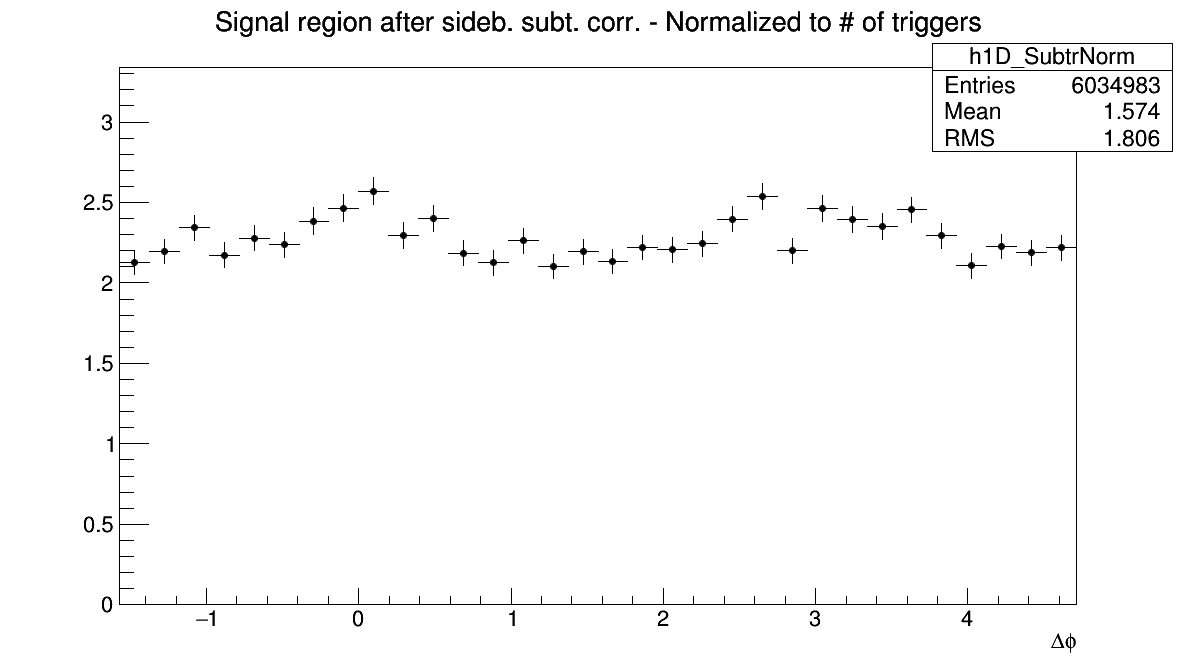
\includegraphics[width=0.31\linewidth, height=0.23\linewidth]{figures/DplusPlotsweff/AzimCorrDistr_Dplus_Canvas_PtIntBins3to4_PoolInt_thr1dotto99dot.png}}
{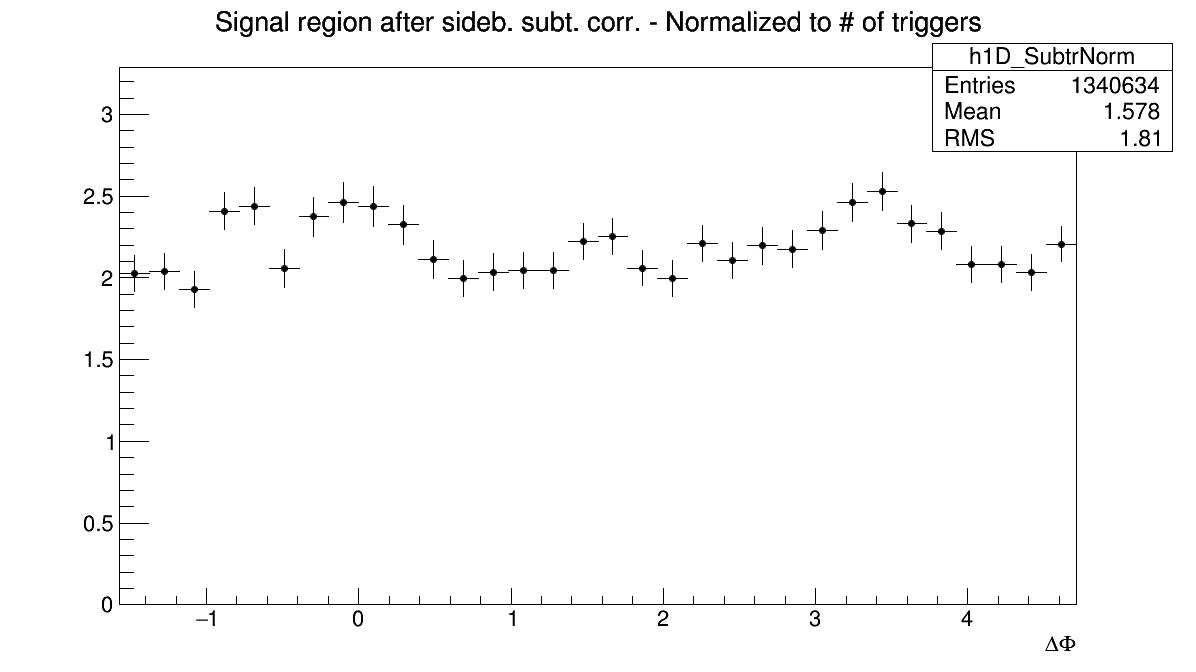
\includegraphics[width=0.31\linewidth, height=0.23\linewidth]{figures/Dstar_wEFF/AzimCorrDistr_Dstar_Canvas_PtIntBins2to3_PoolInt_thr1dotto99dot.png}}
%Pt>2.0GeV/c (LowPt)
{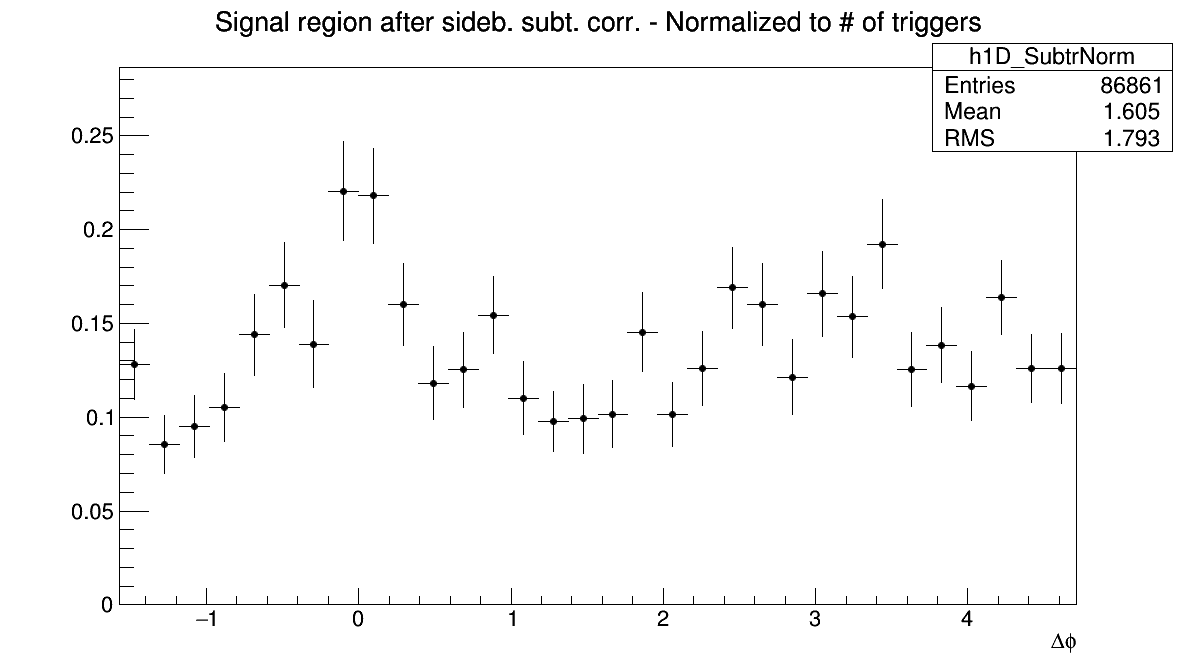
\includegraphics[width=0.31\linewidth, height=0.23\linewidth]{figures/Dzero/AzimCorrDistr_Dzero_Canvas_PtIntBins4to5_PoolInt_thr2dotto99dot.png}}
{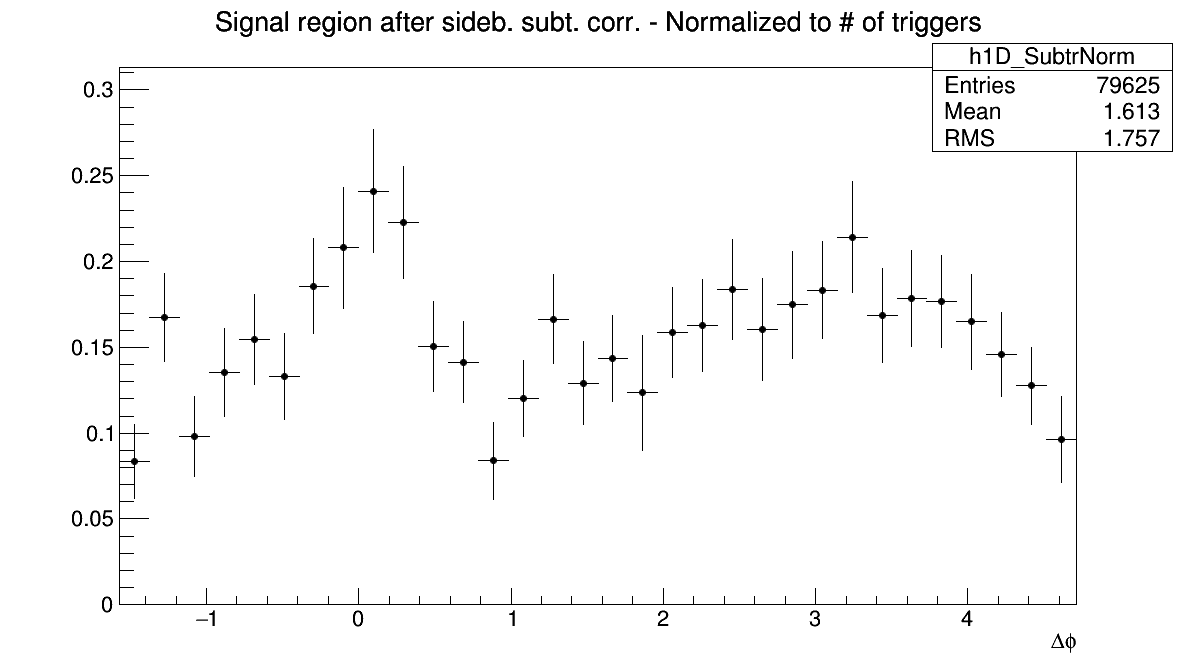
\includegraphics[width=0.31\linewidth, height=0.23\linewidth]{figures/DplusPlotsweff/AzimCorrDistr_Dplus_Canvas_PtIntBins3to4_PoolInt_thr2dotto99dot.png}}
{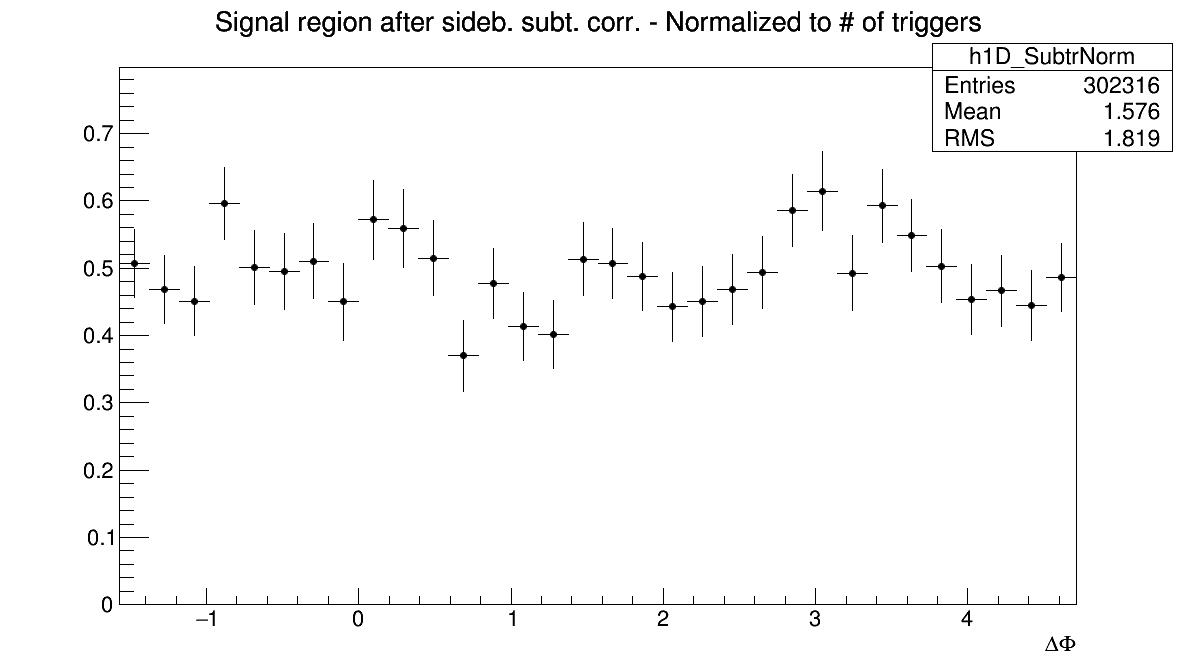
\includegraphics[width=0.31\linewidth, height=0.23\linewidth]{figures/Dstar_wEFF/AzimCorrDistr_Dstar_Canvas_PtIntBins2to3_PoolInt_thr2dotto99dot.png}}
%Pt>3.0GeV/c (LowPt)
{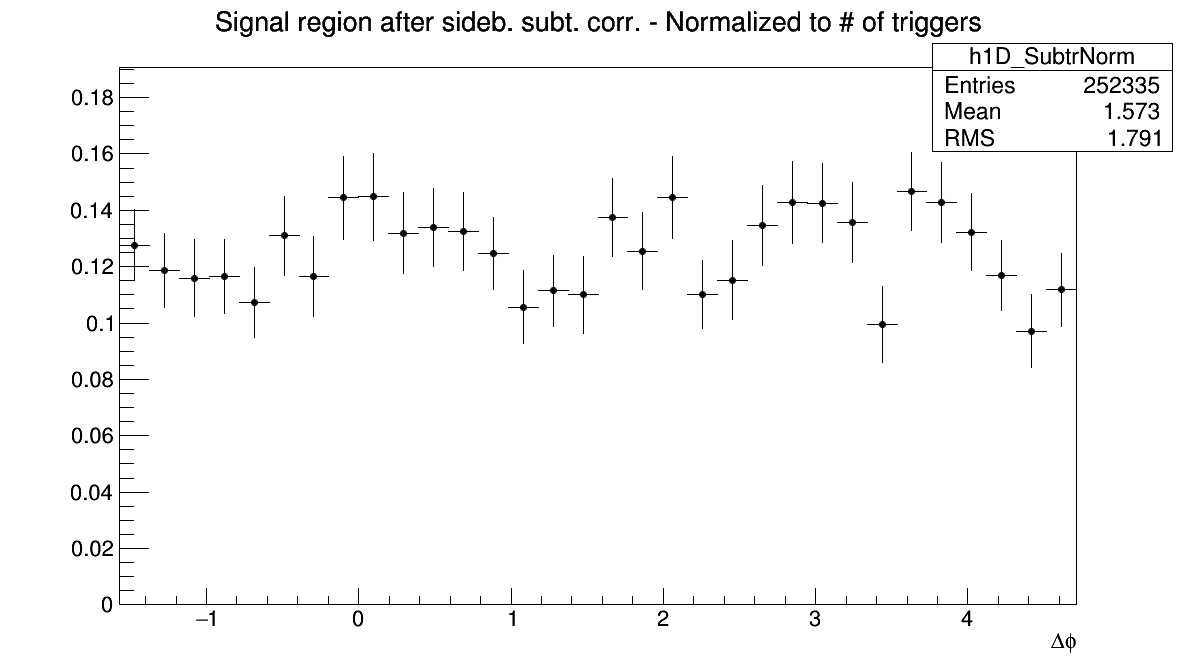
\includegraphics[width=0.31\linewidth, height=0.23\linewidth]{figures/Dzero/AzimCorrDistr_Dzero_Canvas_PtIntBins4to5_PoolInt_thr3dotto99dot.png}}
{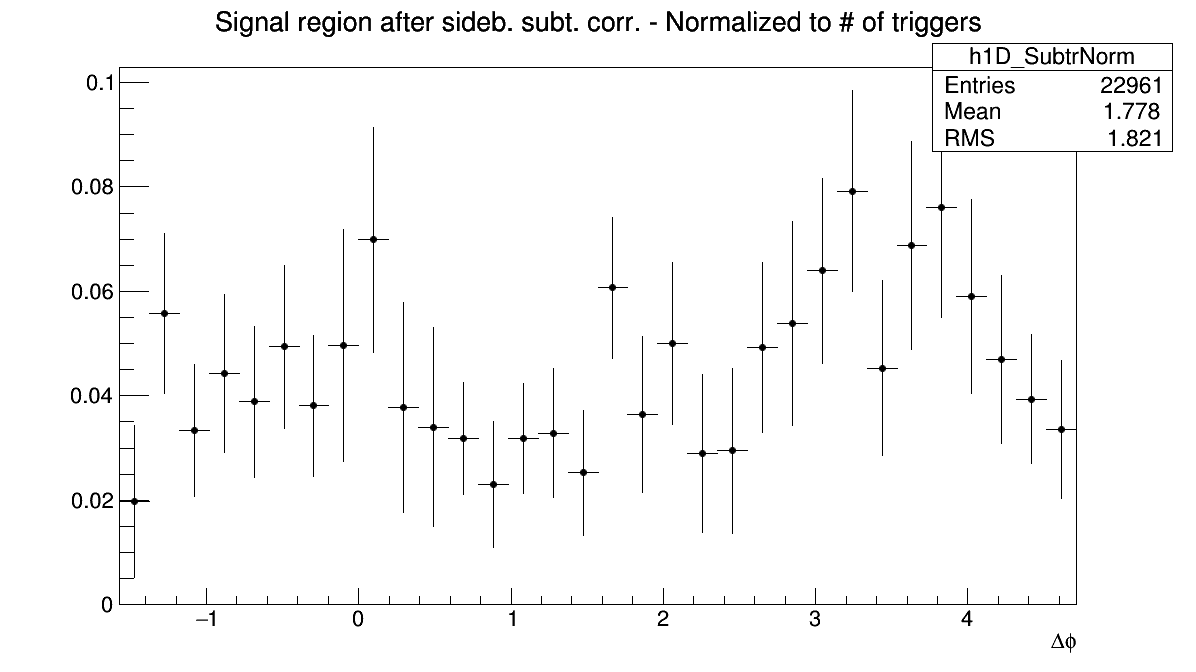
\includegraphics[width=0.31\linewidth, height=0.23\linewidth]{figures/DplusPlotsweff/AzimCorrDistr_Dplus_Canvas_PtIntBins3to4_PoolInt_thr3dotto99dot.png}}
{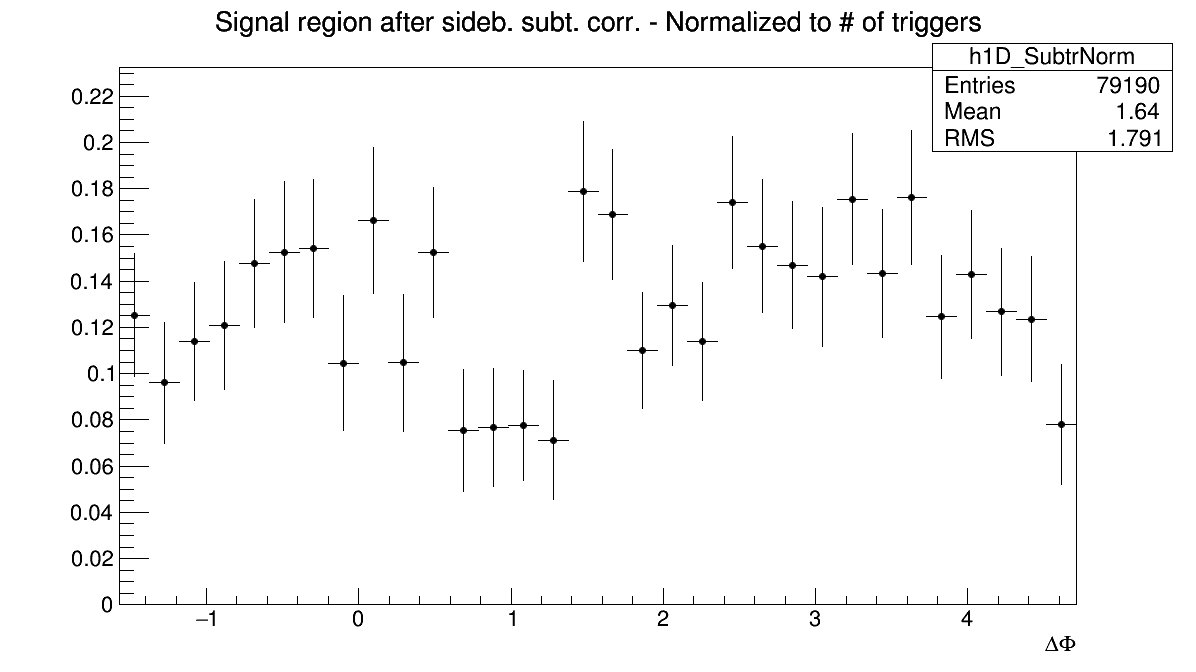
\includegraphics[width=0.31\linewidth, height=0.23\linewidth]{figures/Dstar_wEFF/AzimCorrDistr_Dstar_Canvas_PtIntBins2to3_PoolInt_thr3dotto99dot.png}}
%Pt>0.3-1.0GeV/c (LowPt)
{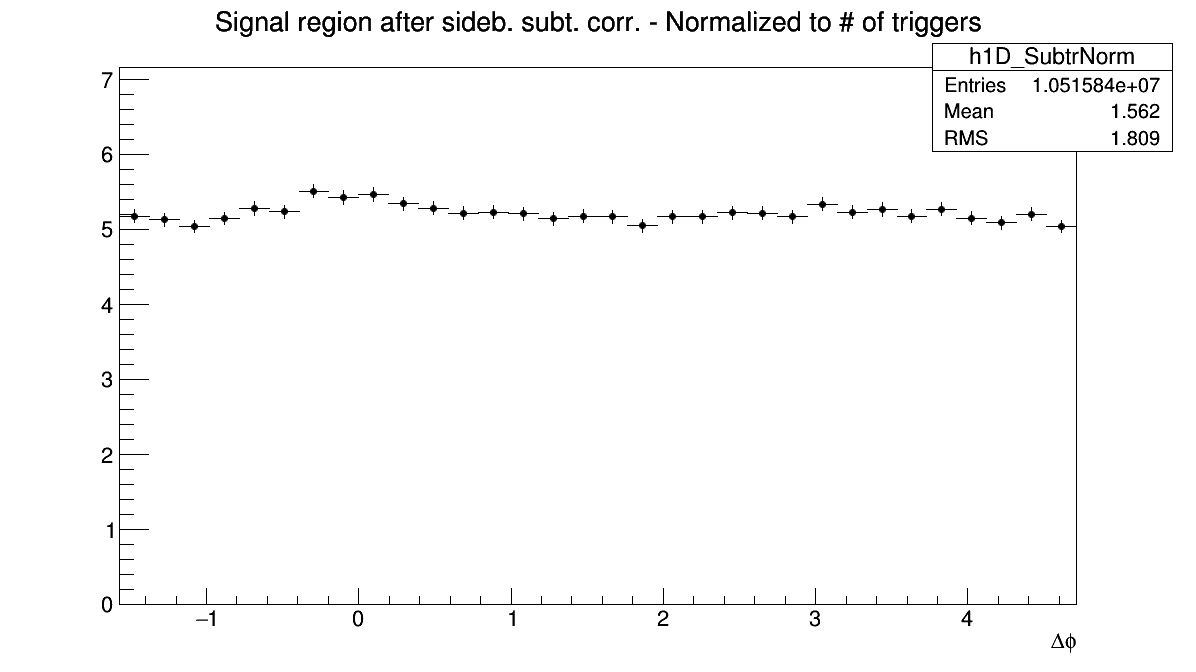
\includegraphics[width=0.31\linewidth, height=0.23\linewidth]{figures/Dzero/AzimCorrDistr_Dzero_Canvas_PtIntBins4to5_PoolInt_thrdot3to1dot.png}}
{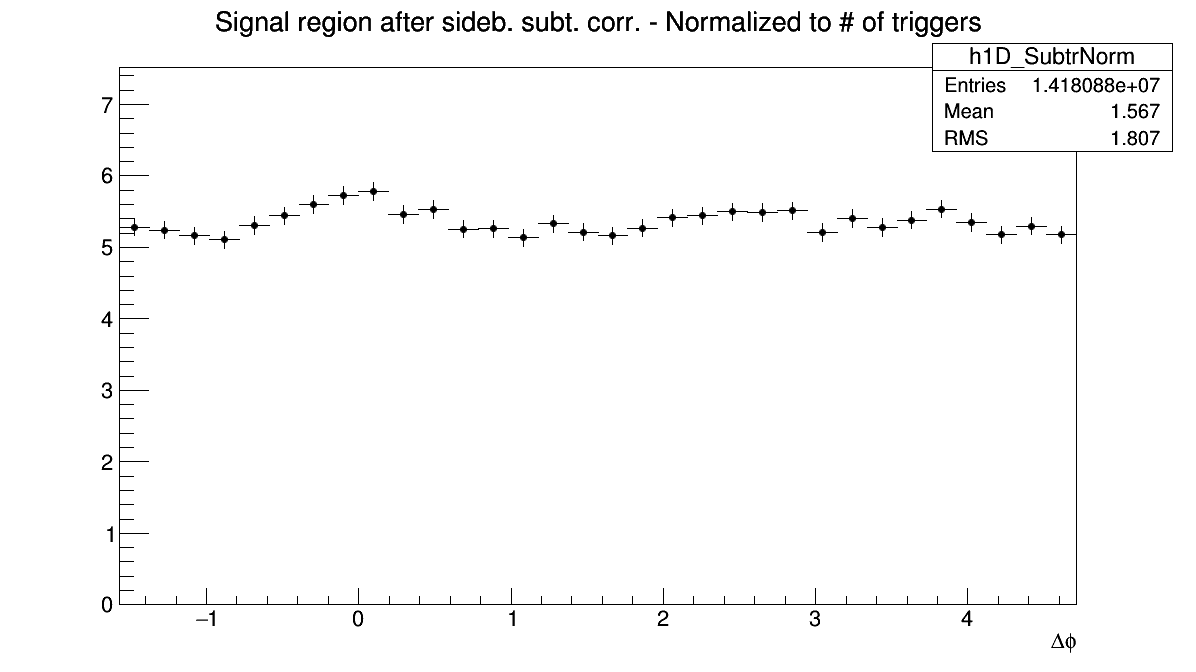
\includegraphics[width=0.31\linewidth, height=0.23\linewidth]{figures/DplusPlotsweff/AzimCorrDistr_Dplus_Canvas_PtIntBins3to4_PoolInt_thrdot3to1dot.png}}
{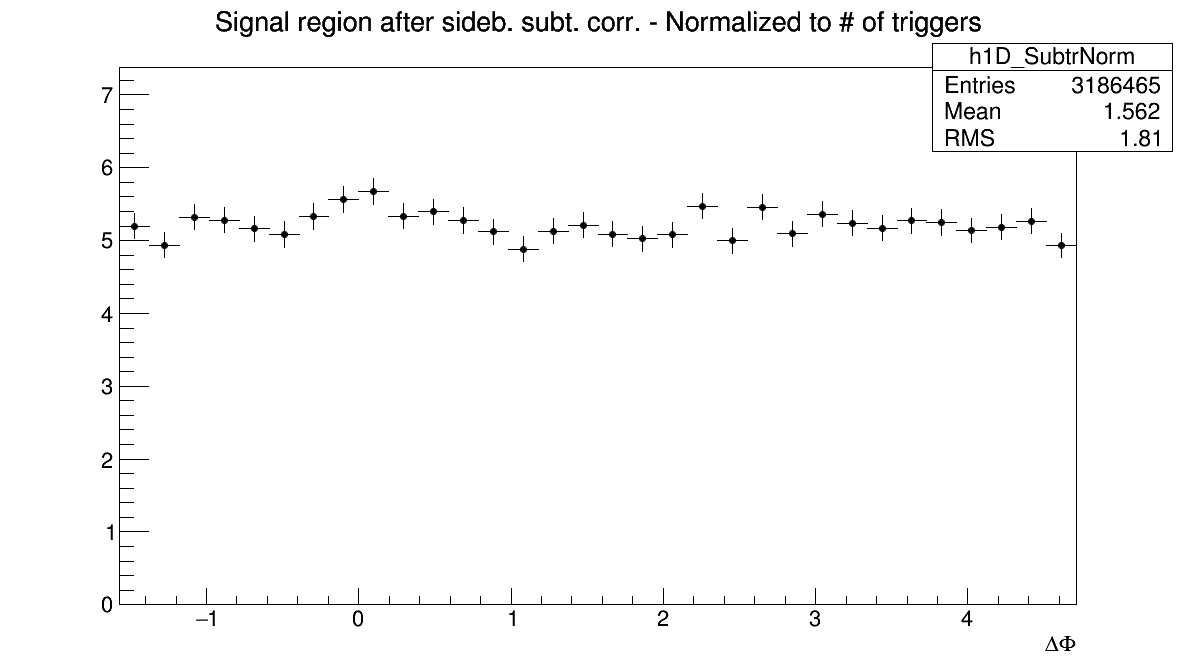
\includegraphics[width=0.31\linewidth, height=0.23\linewidth]{figures/Dstar_wEFF/AzimCorrDistr_Dstar_Canvas_PtIntBins2to3_PoolInt_thrdot3to1dot.png}}
%Pt>1.0-2.0GeV/c (LowPt)
{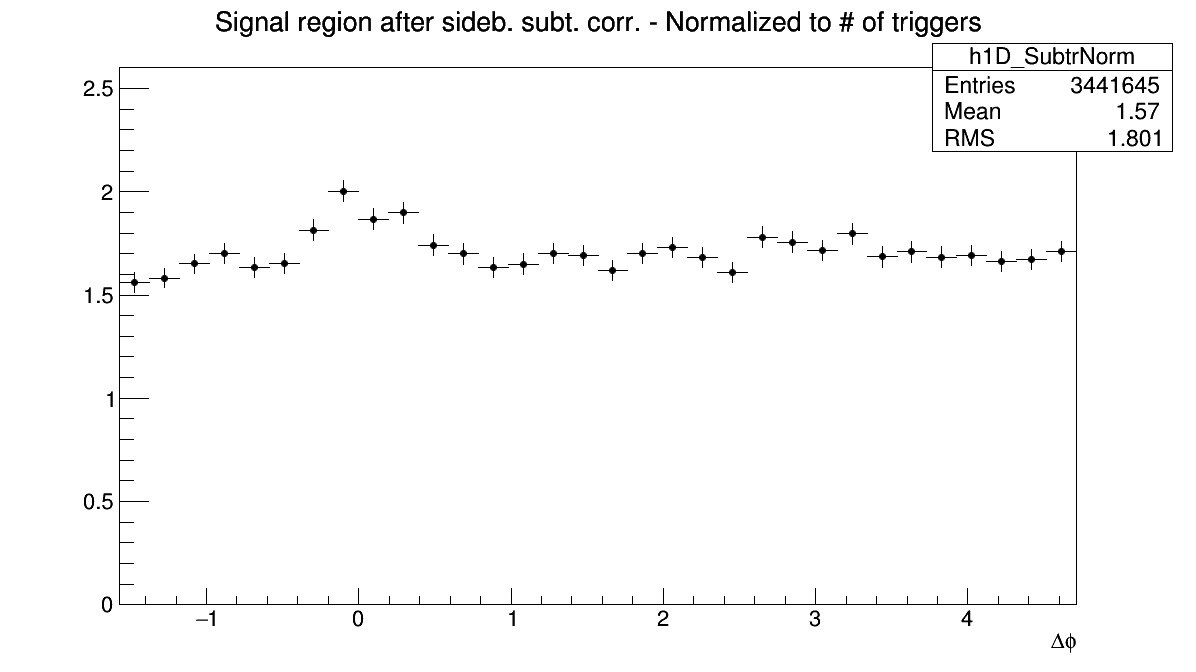
\includegraphics[width=0.31\linewidth, height=0.23\linewidth]{figures/Dzero/AzimCorrDistr_Dzero_Canvas_PtIntBins4to5_PoolInt_thr1dotto2dot.png}}
{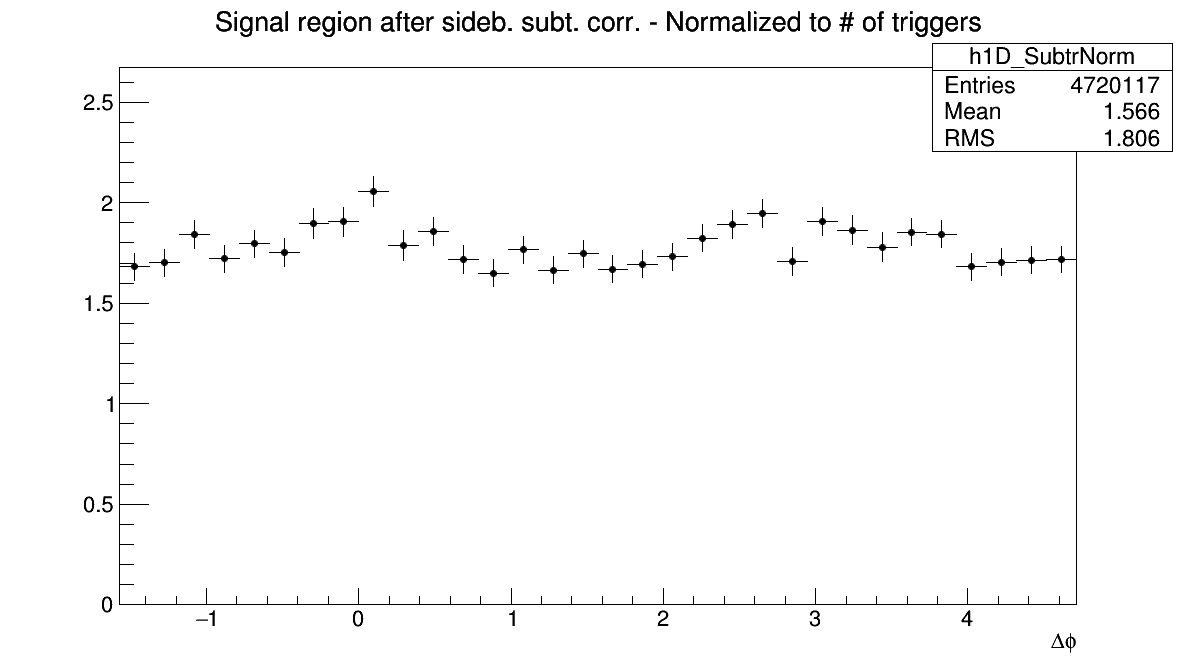
\includegraphics[width=0.31\linewidth, height=0.23\linewidth]{figures/DplusPlotsweff/AzimCorrDistr_Dplus_Canvas_PtIntBins3to4_PoolInt_thr1dotto2dot.png}}
{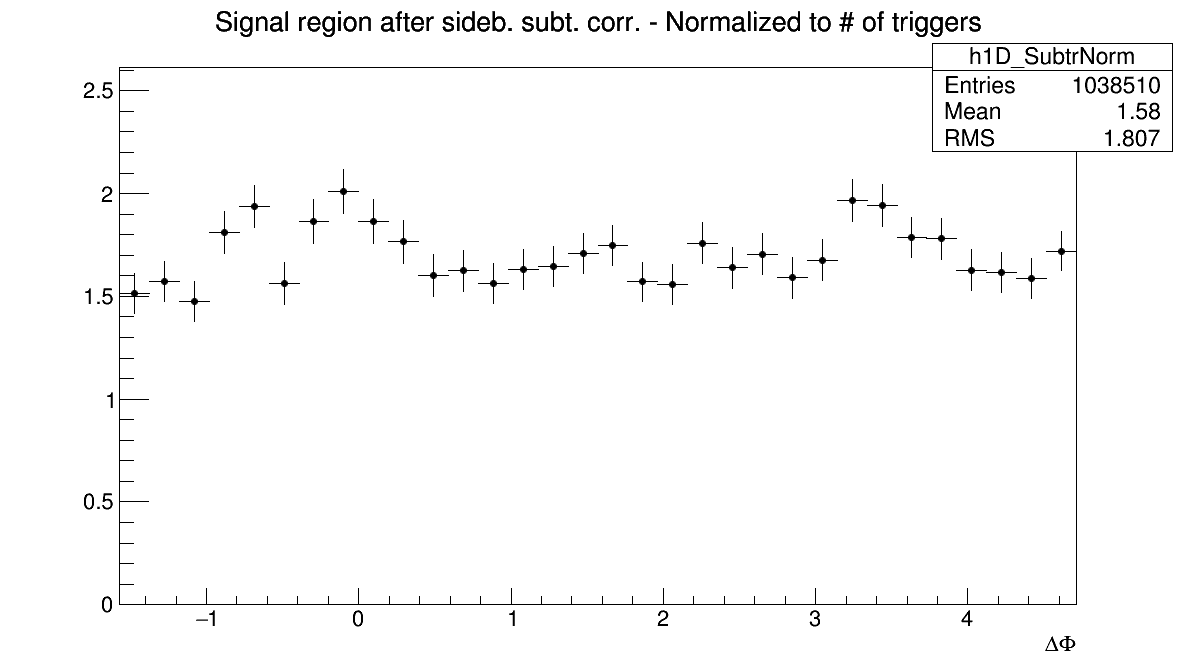
\includegraphics[width=0.31\linewidth, height=0.23\linewidth]{figures/Dstar_wEFF/AzimCorrDistr_Dstar_Canvas_PtIntBins2to3_PoolInt_thr1dotto2dot.png}}
\end{figure}
\begin{figure}[!htbp]
\centering
%Pt>2.0-3.0GeV/c (LowPt)
{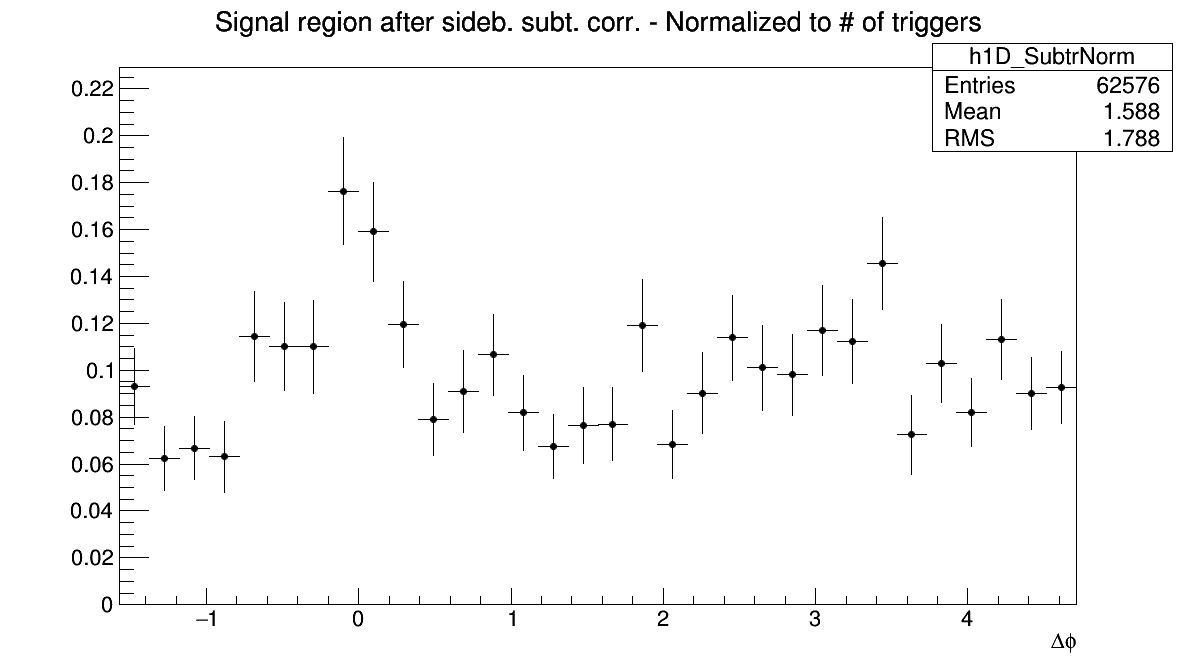
\includegraphics[width=0.31\linewidth, height=0.23\linewidth]{figures/Dzero/AzimCorrDistr_Dzero_Canvas_PtIntBins4to5_PoolInt_thr2dotto3dot.png}}
{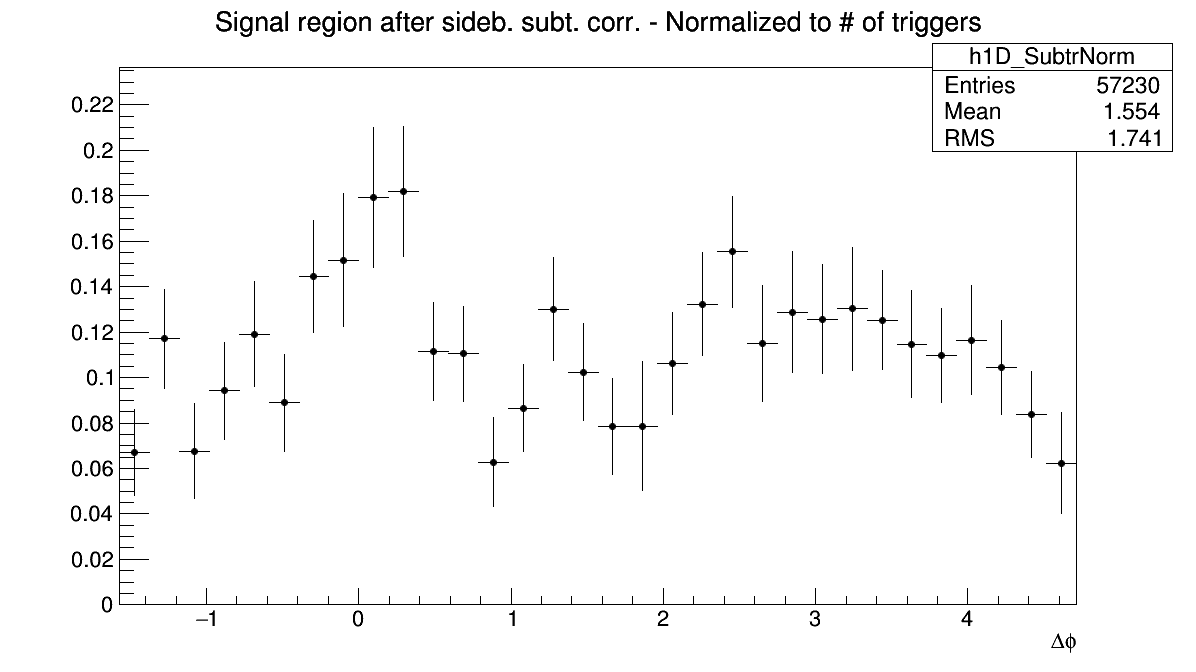
\includegraphics[width=0.31\linewidth, height=0.23\linewidth]{figures/DplusPlotsweff/AzimCorrDistr_Dplus_Canvas_PtIntBins3to4_PoolInt_thr2dotto3dot.png}}
{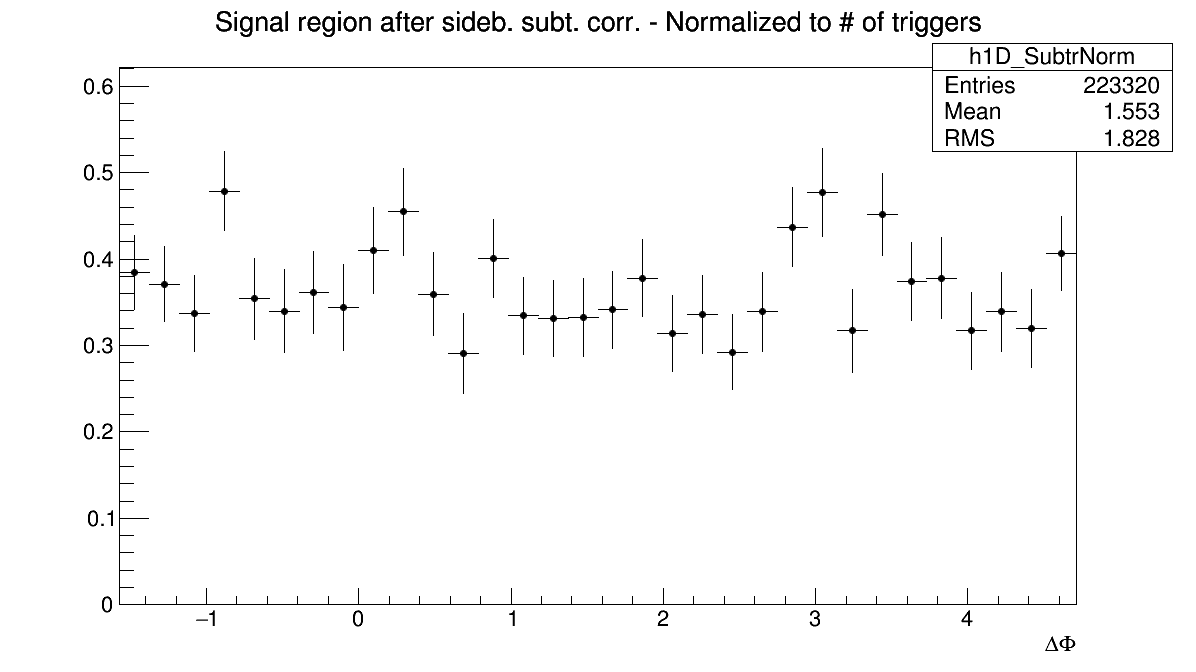
\includegraphics[width=0.31\linewidth, height=0.23\linewidth]{figures/Dstar_wEFF/AzimCorrDistr_Dstar_Canvas_PtIntBins2to3_PoolInt_thr2dotto3dot.png}}
% Pt>0.3 (MidPt)
{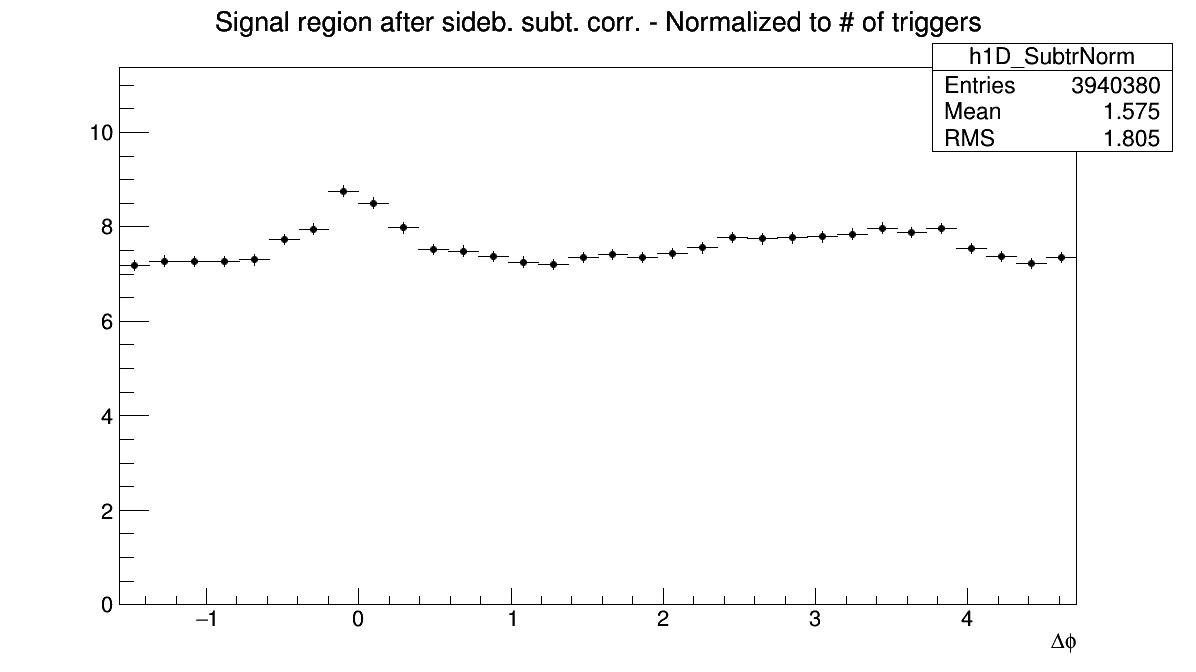
\includegraphics[width=0.31\linewidth, height=0.23\linewidth]{figures/Dzero/AzimCorrDistr_Dzero_Canvas_PtIntBins6to8_PoolInt_thrdot3to99dot.png}}
{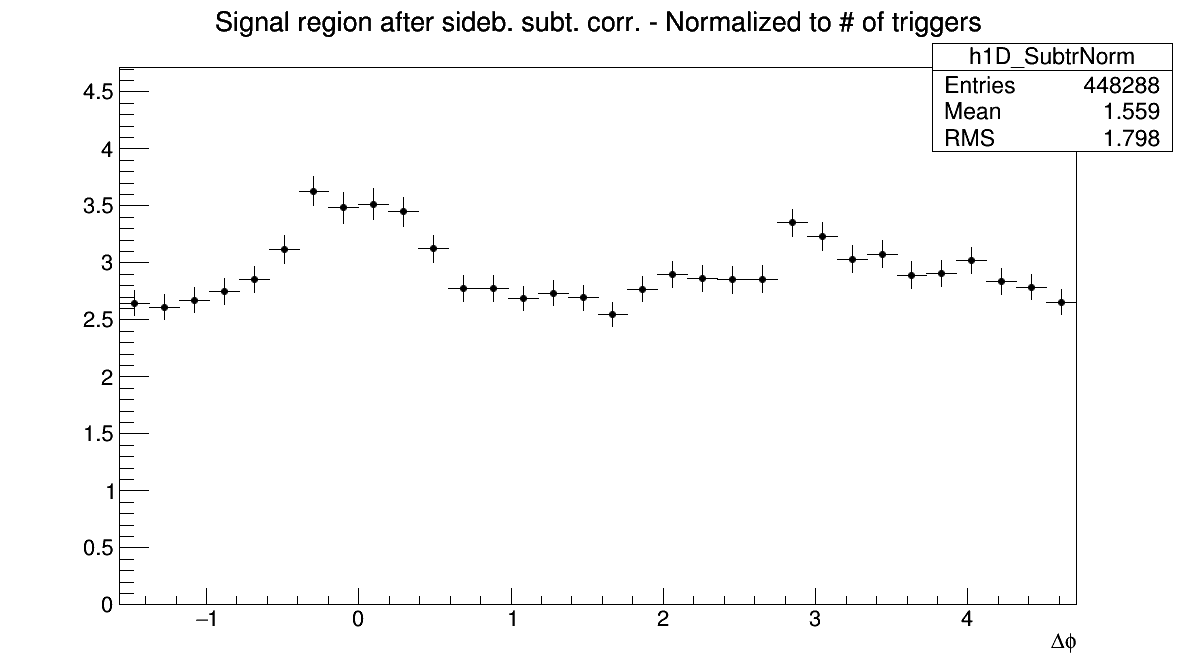
\includegraphics[width=0.31\linewidth, height=0.23\linewidth]{figures/DplusPlotsweff/AzimCorrDistr_Dplus_Canvas_PtIntBins5to7_PoolInt_thrdot3to99dot.png}}
{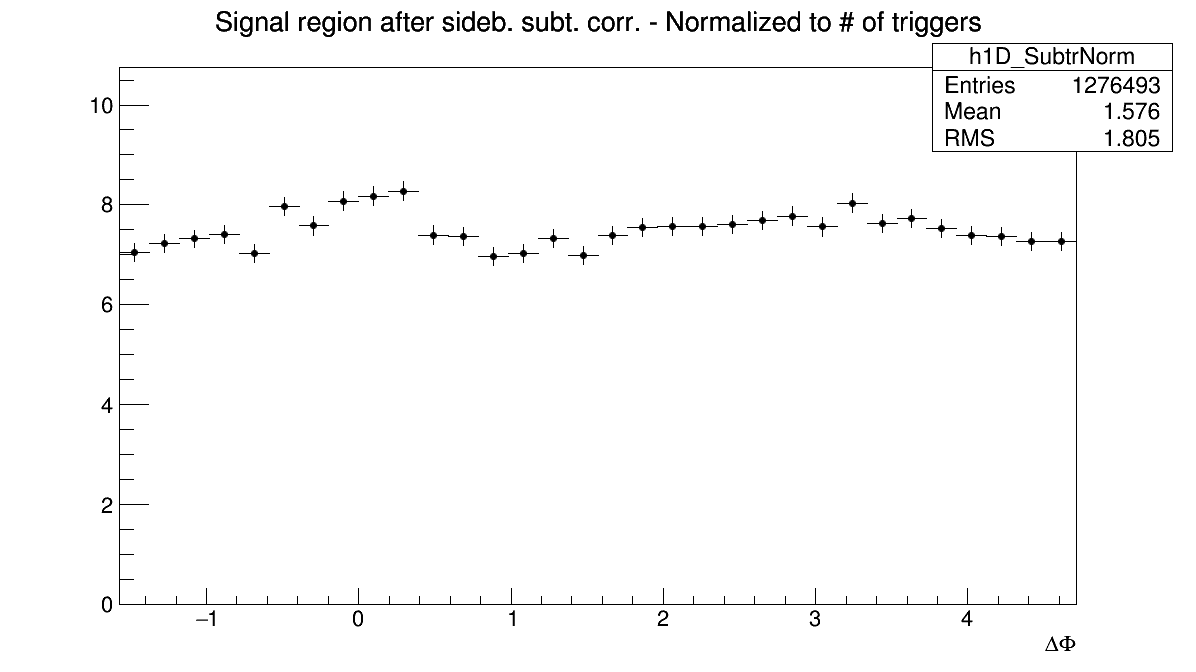
\includegraphics[width=0.31\linewidth, height=0.23\linewidth]{figures/Dstar_wEFF/AzimCorrDistr_Dstar_Canvas_PtIntBins4to6_PoolInt_thrdot3to99dot.png}}
% Pt>1.0 (MidPt)
{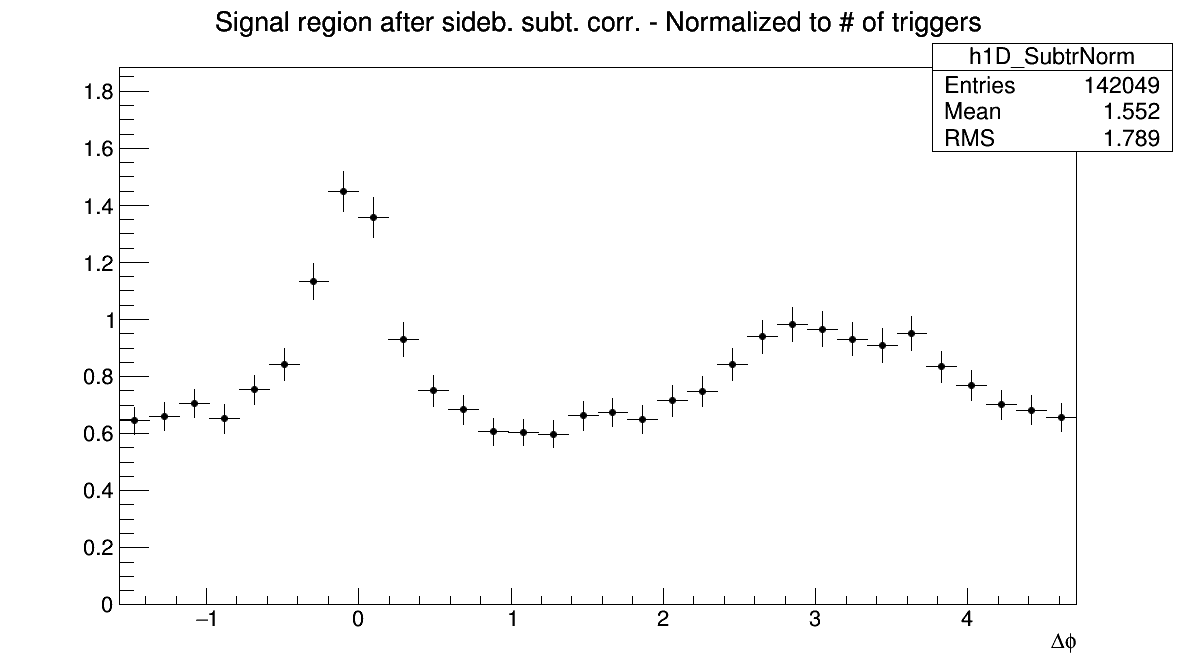
\includegraphics[width=0.31\linewidth, height=0.23\linewidth]{figures/Dzero/AzimCorrDistr_Dzero_Canvas_PtIntBins6to8_PoolInt_thr1dotto99dot.png}}
{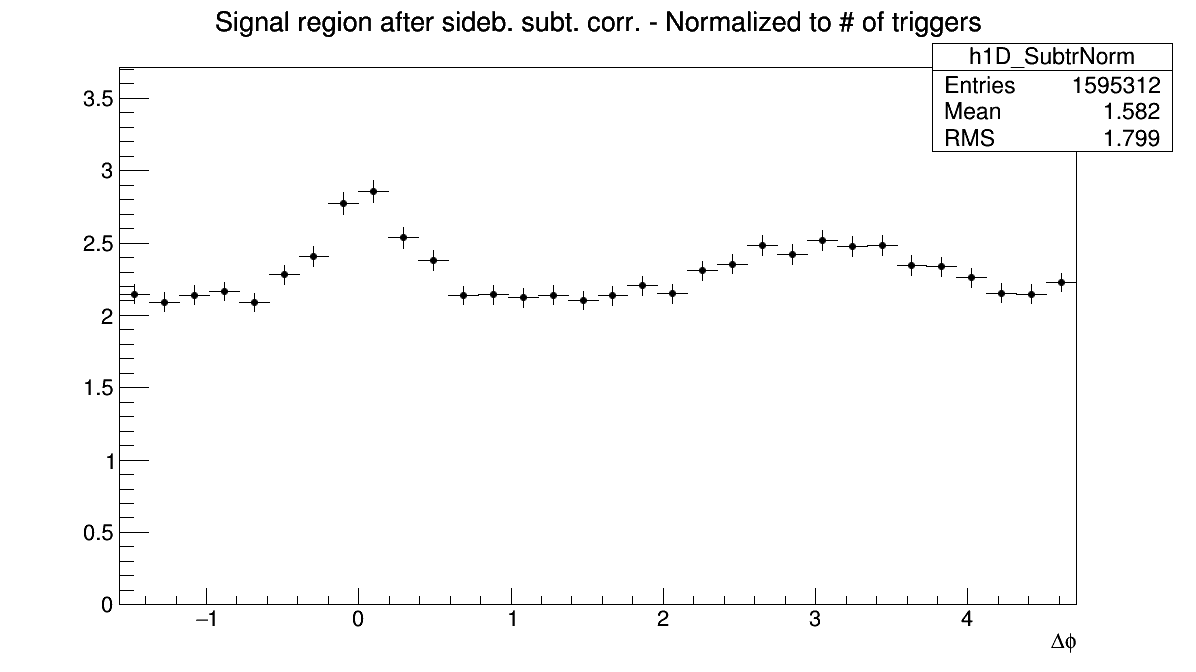
\includegraphics[width=0.31\linewidth, height=0.23\linewidth]{figures/DplusPlotsweff/AzimCorrDistr_Dplus_Canvas_PtIntBins5to7_PoolInt_thr1dotto99dot.png}}
{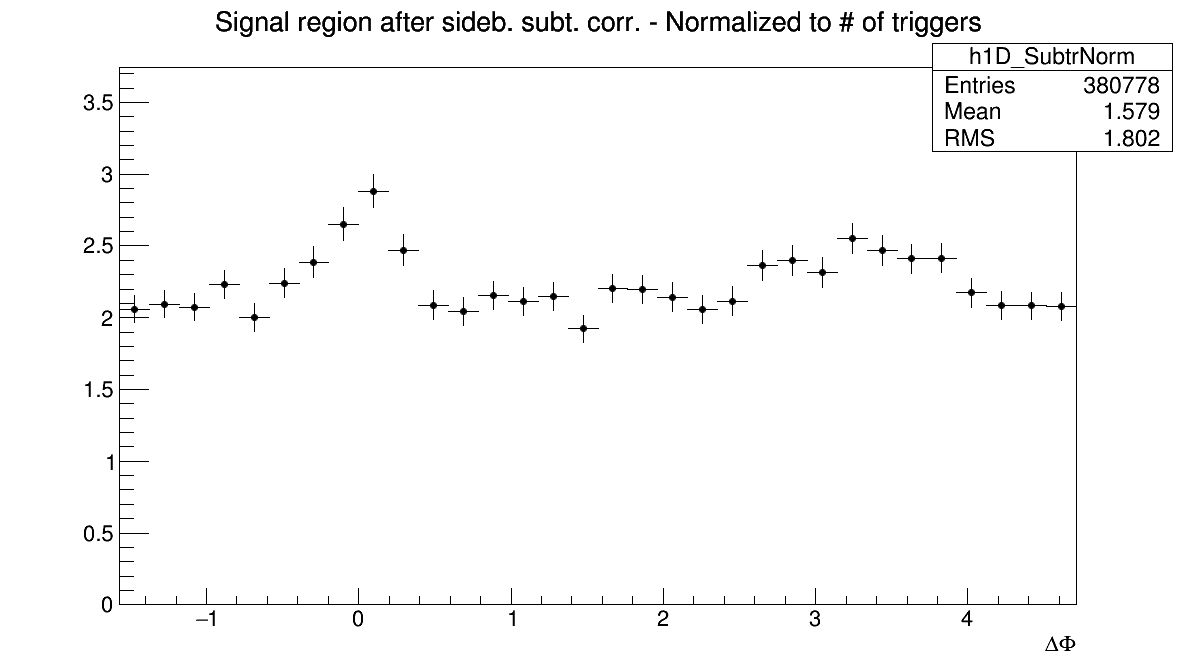
\includegraphics[width=0.31\linewidth, height=0.23\linewidth]{figures/Dstar_wEFF/AzimCorrDistr_Dstar_Canvas_PtIntBins4to6_PoolInt_thr1dotto99dot.png}}
% Pt>2.0 (MidPt)
{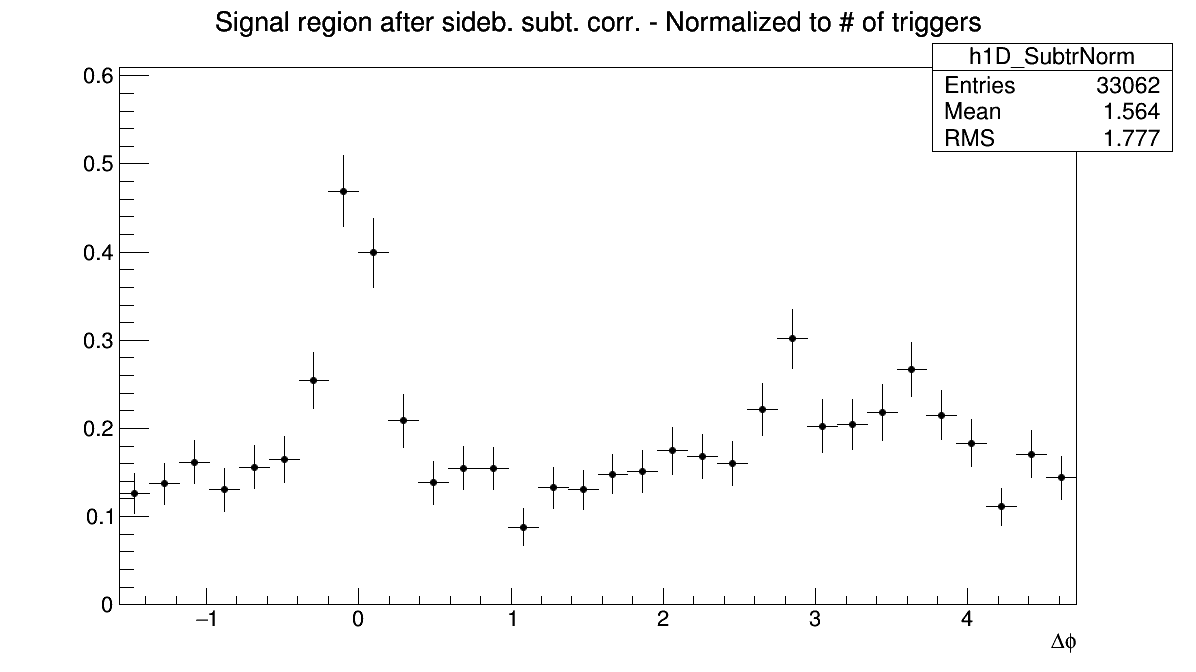
\includegraphics[width=0.31\linewidth, height=0.23\linewidth]{figures/Dzero/AzimCorrDistr_Dzero_Canvas_PtIntBins6to8_PoolInt_thr2dotto99dot.png}}
{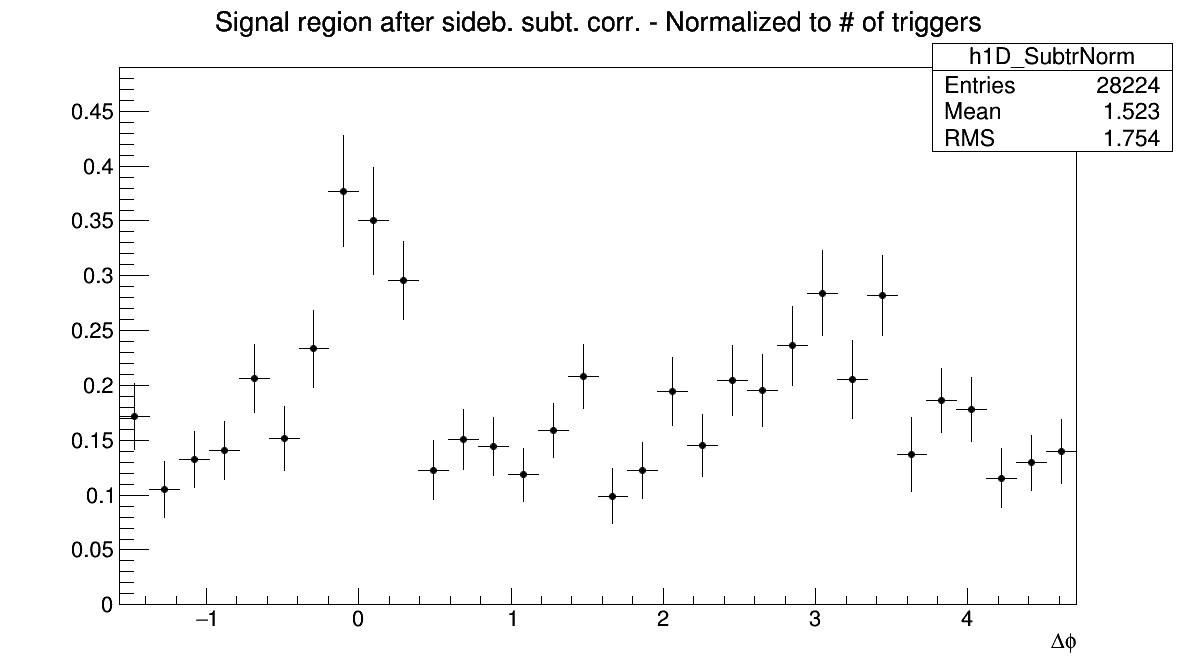
\includegraphics[width=0.31\linewidth, height=0.23\linewidth]{figures/DplusPlotsweff/AzimCorrDistr_Dplus_Canvas_PtIntBins5to7_PoolInt_thr2dotto99dot.png}}
{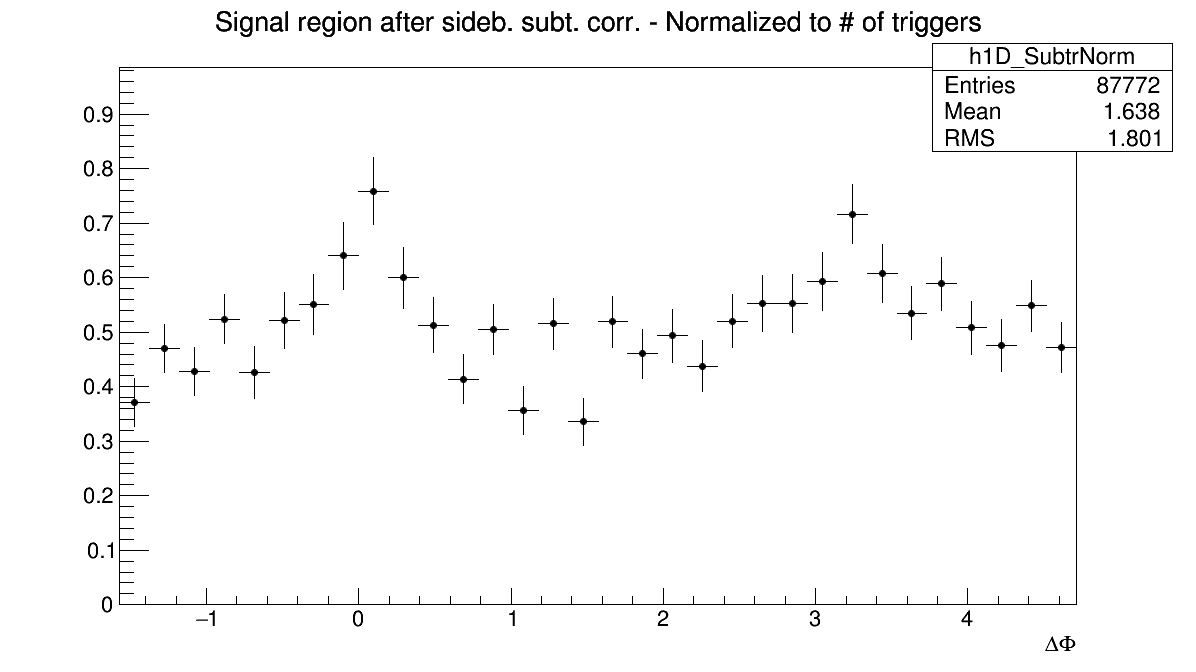
\includegraphics[width=0.31\linewidth, height=0.23\linewidth]{figures/Dstar_wEFF/AzimCorrDistr_Dstar_Canvas_PtIntBins4to6_PoolInt_thr2dotto99dot.png}}
% Pt>3.0 (MidPt)
{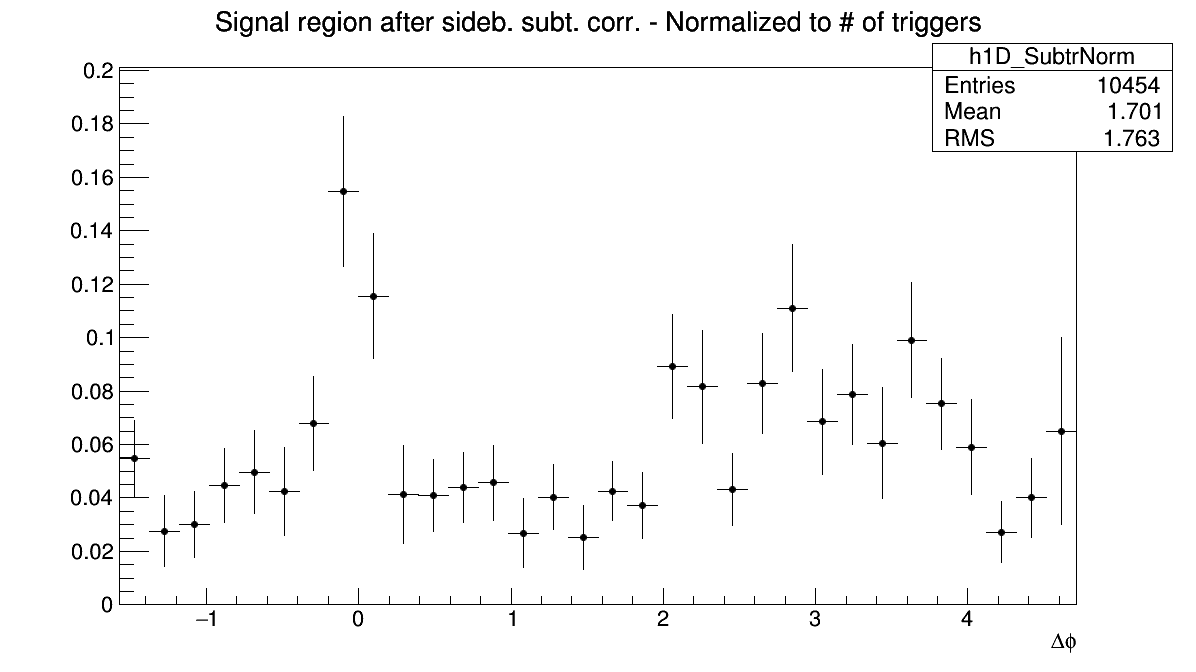
\includegraphics[width=0.31\linewidth, height=0.23\linewidth]{figures/Dzero/AzimCorrDistr_Dzero_Canvas_PtIntBins6to8_PoolInt_thr3dotto99dot.png}}
{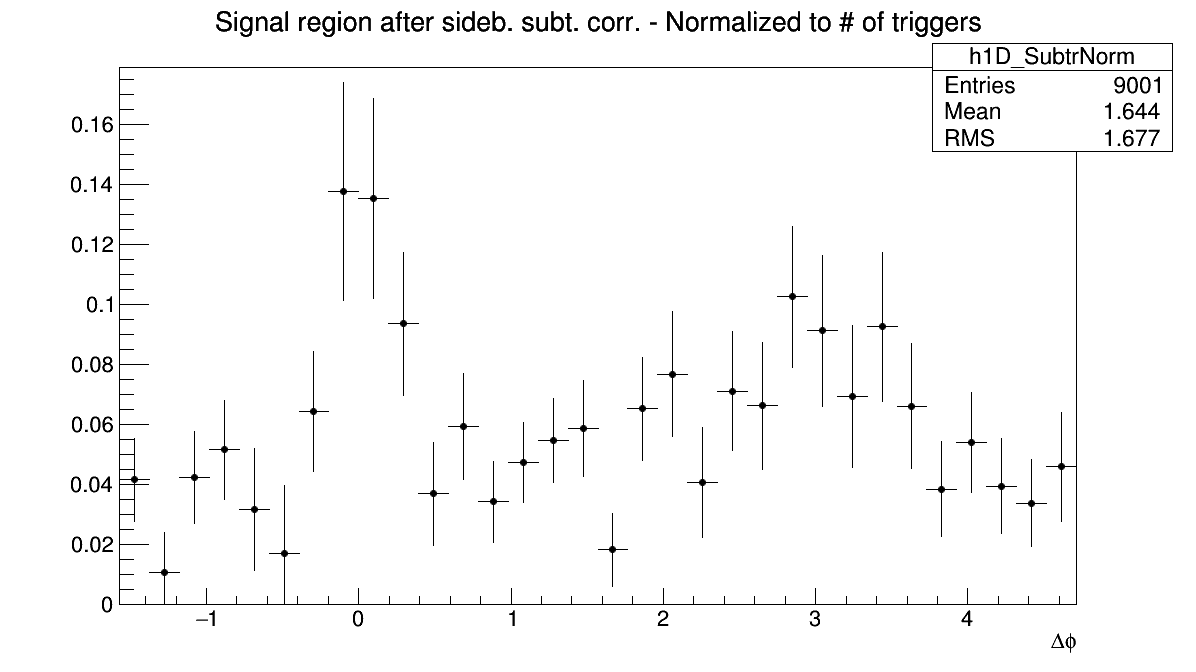
\includegraphics[width=0.31\linewidth, height=0.23\linewidth]{figures/DplusPlotsweff/AzimCorrDistr_Dplus_Canvas_PtIntBins5to7_PoolInt_thr3dotto99dot.png}}
{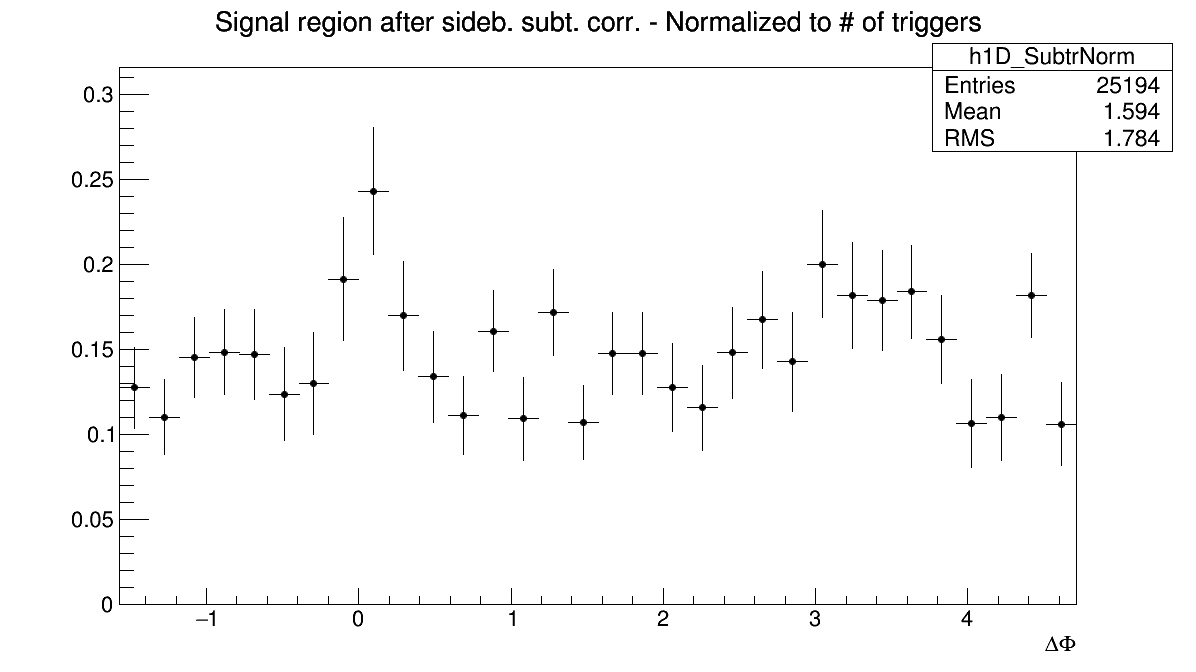
\includegraphics[width=0.31\linewidth, height=0.23\linewidth]{figures/Dstar_wEFF/AzimCorrDistr_Dstar_Canvas_PtIntBins4to6_PoolInt_thr3dotto99dot.png}}
% Pt>0.3-1.0 (MidPt)
{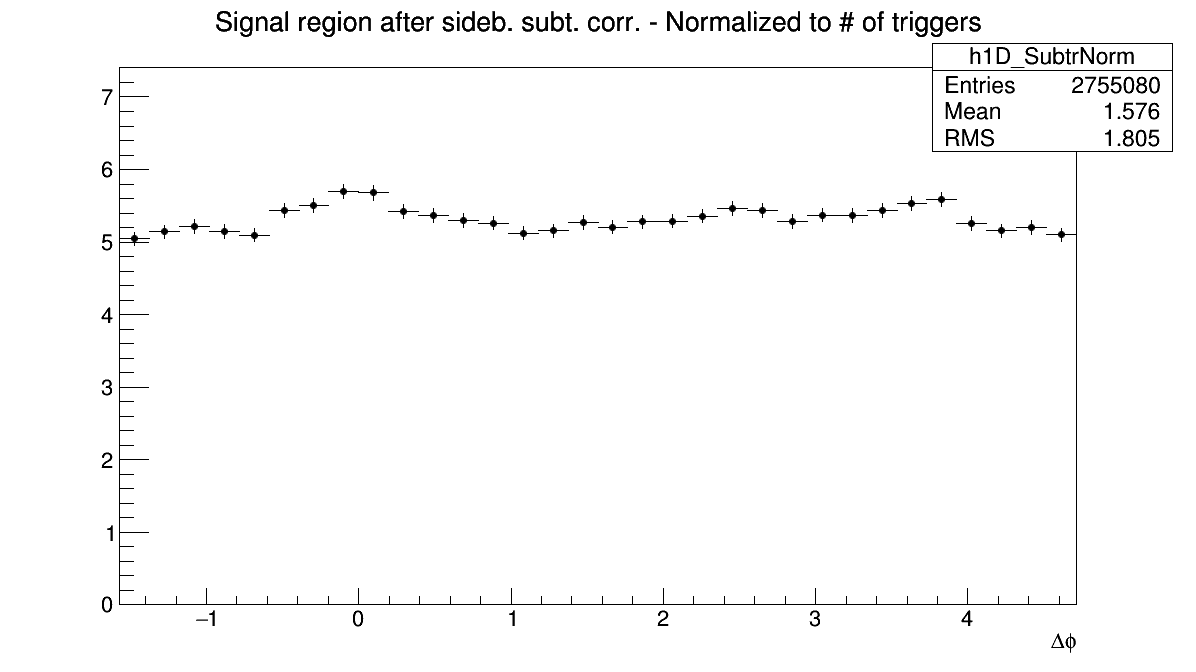
\includegraphics[width=0.31\linewidth, height=0.23\linewidth]{figures/Dzero/AzimCorrDistr_Dzero_Canvas_PtIntBins6to8_PoolInt_thrdot3to1dot.png}}
{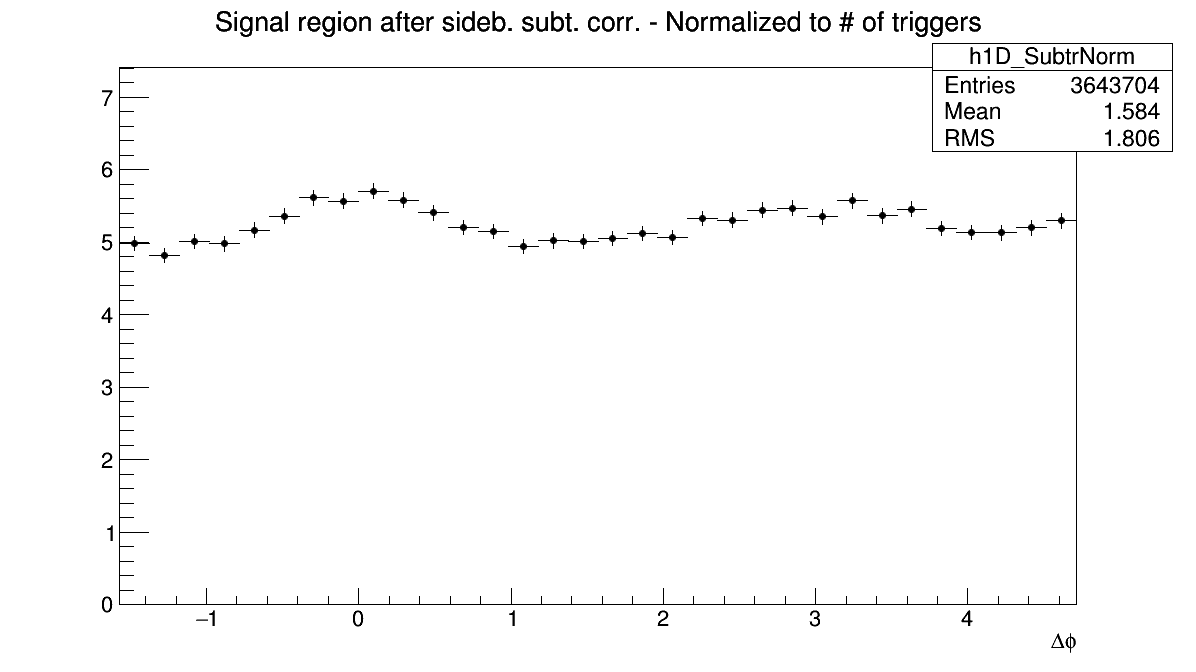
\includegraphics[width=0.31\linewidth, height=0.23\linewidth]{figures/DplusPlotsweff/AzimCorrDistr_Dplus_Canvas_PtIntBins5to7_PoolInt_thrdot3to1dot.png}}
{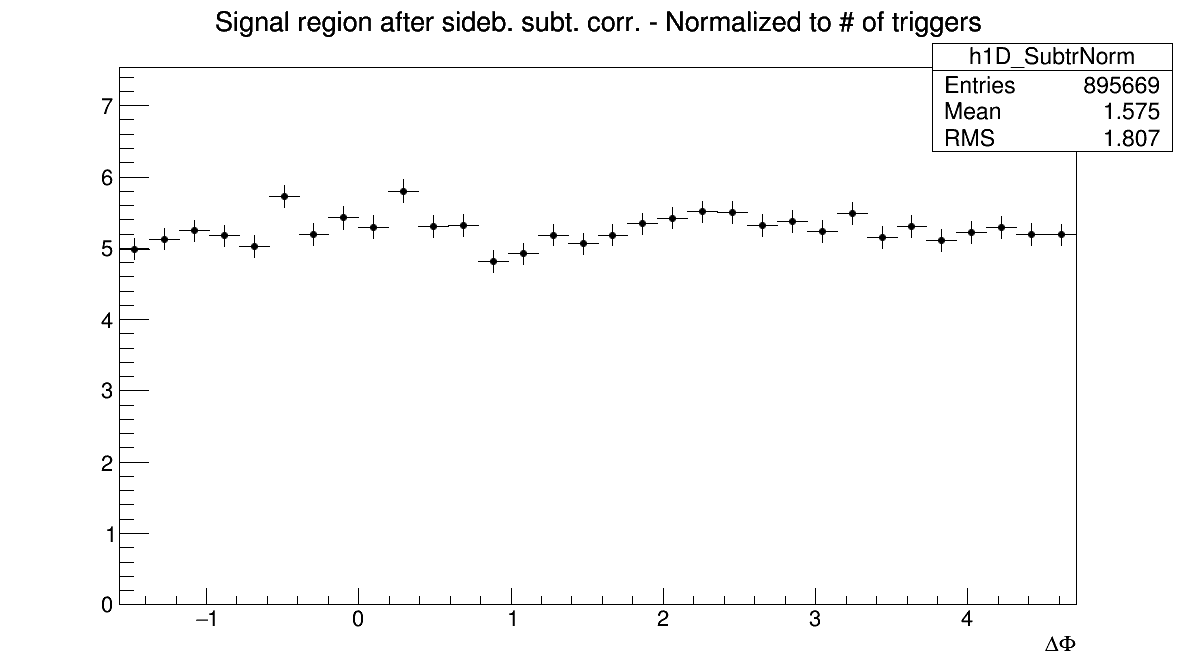
\includegraphics[width=0.31\linewidth, height=0.23\linewidth]{figures/Dstar_wEFF/AzimCorrDistr_Dstar_Canvas_PtIntBins4to6_PoolInt_thrdot3to1dot.png}}
\end{figure}
\begin{figure}[!htbp]
\centering
% Pt>1.0-2.0 (MidPt)
{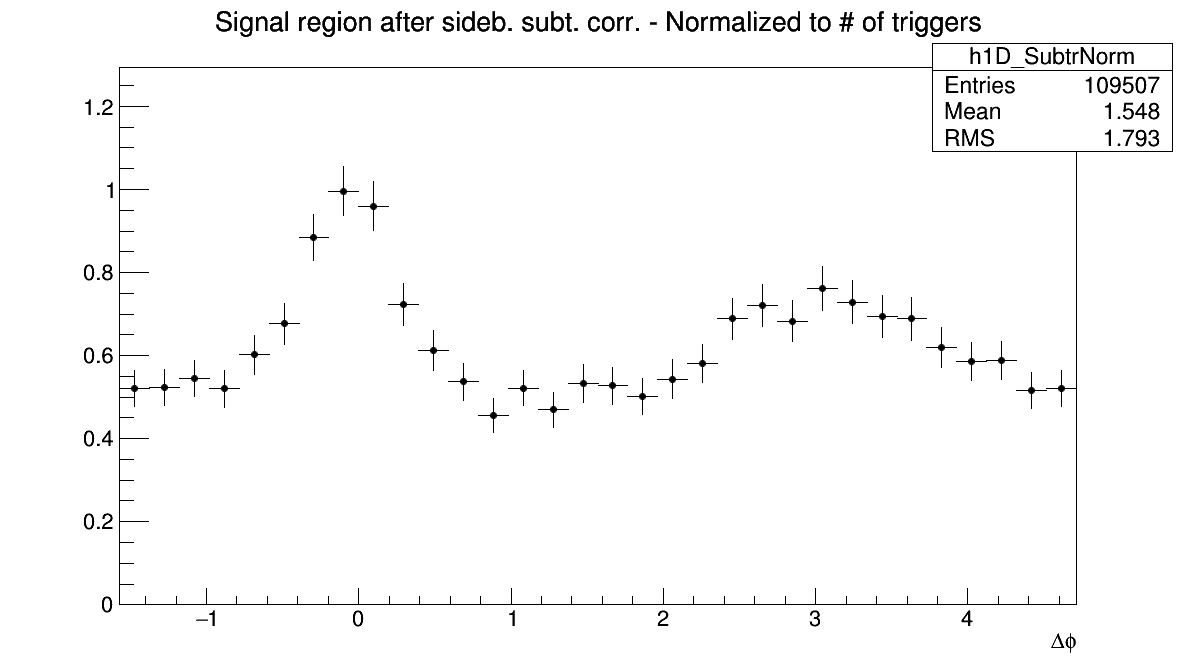
\includegraphics[width=0.31\linewidth, height=0.23\linewidth]{figures/Dzero/AzimCorrDistr_Dzero_Canvas_PtIntBins6to8_PoolInt_thr1dotto2dot.png}}
{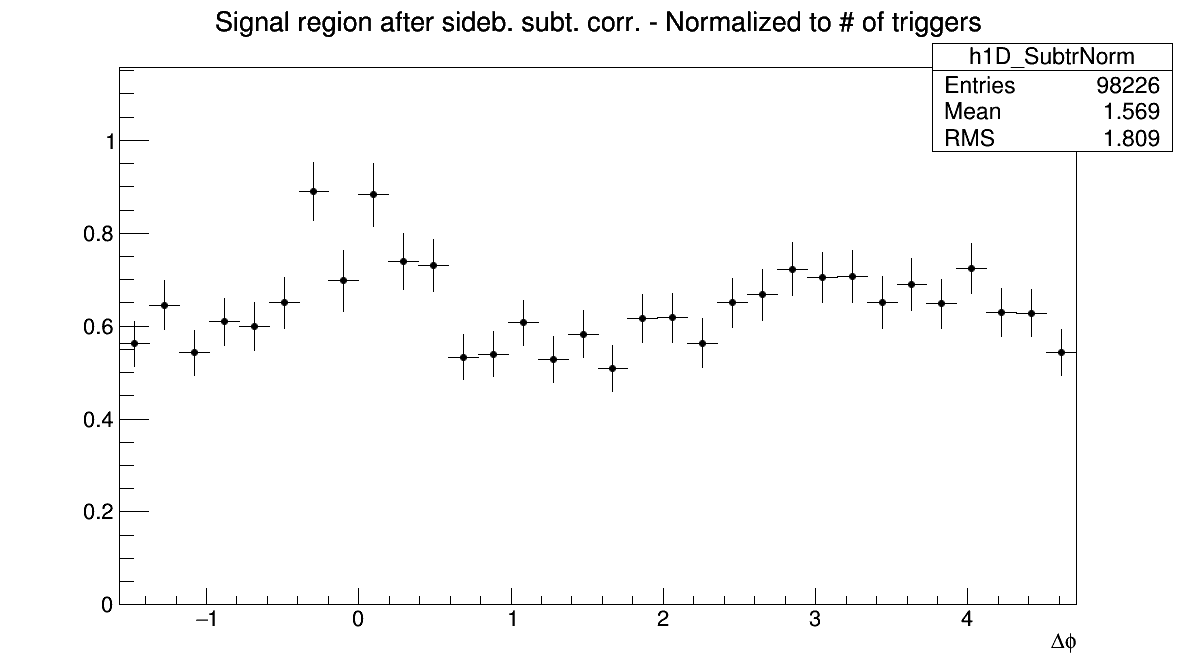
\includegraphics[width=0.31\linewidth, height=0.23\linewidth]{figures/DplusPlotsweff/AzimCorrDistr_Dplus_Canvas_PtIntBins5to7_PoolInt_thr1dotto2dot.png}}
{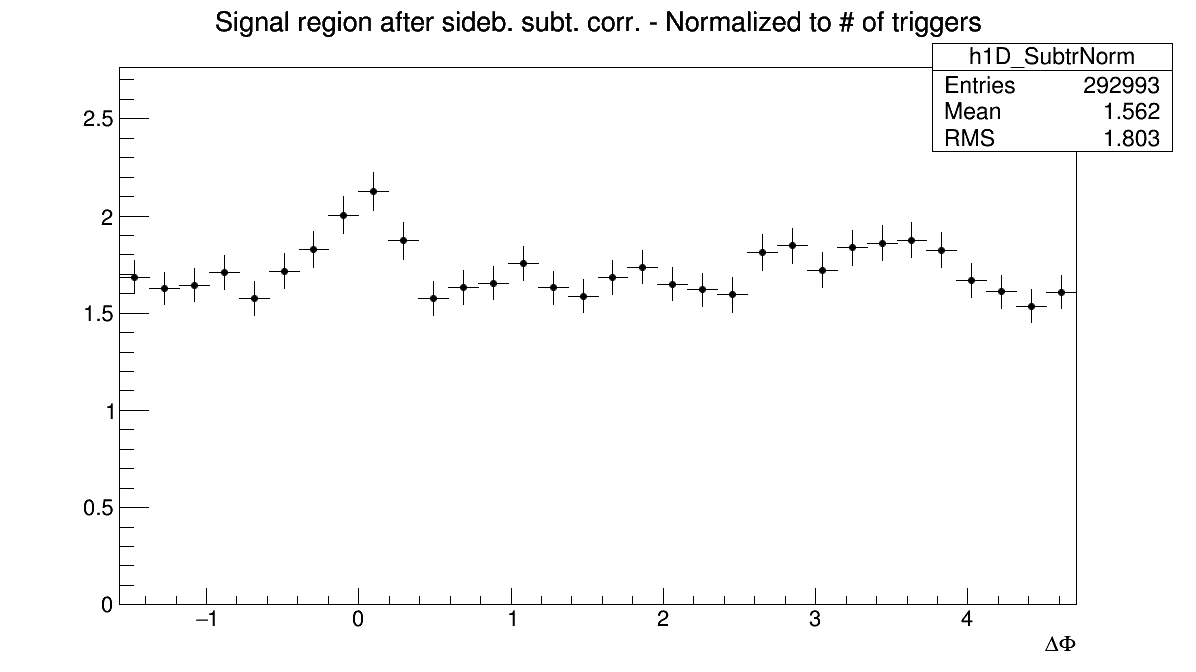
\includegraphics[width=0.31\linewidth, height=0.23\linewidth]{figures/Dstar_wEFF/AzimCorrDistr_Dstar_Canvas_PtIntBins4to6_PoolInt_thr1dotto2dot.png}}
% Pt>2.0-3.0 (MidPt)
{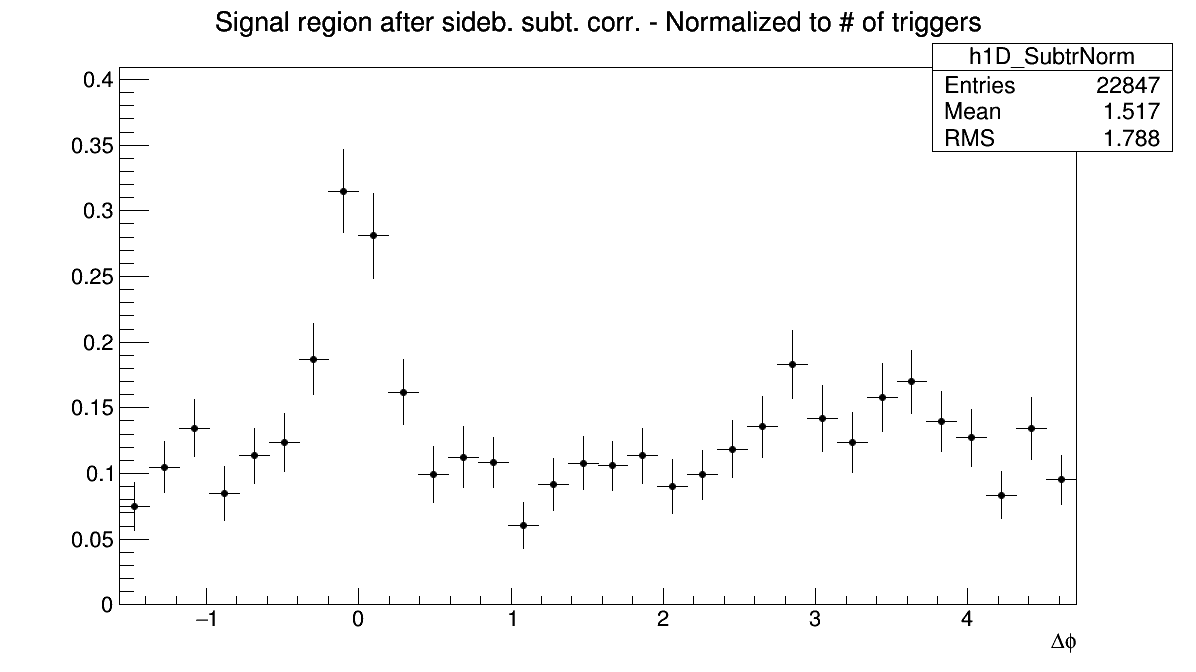
\includegraphics[width=0.31\linewidth, height=0.23\linewidth]{figures/Dzero/AzimCorrDistr_Dzero_Canvas_PtIntBins6to8_PoolInt_thr2dotto3dot.png}}
{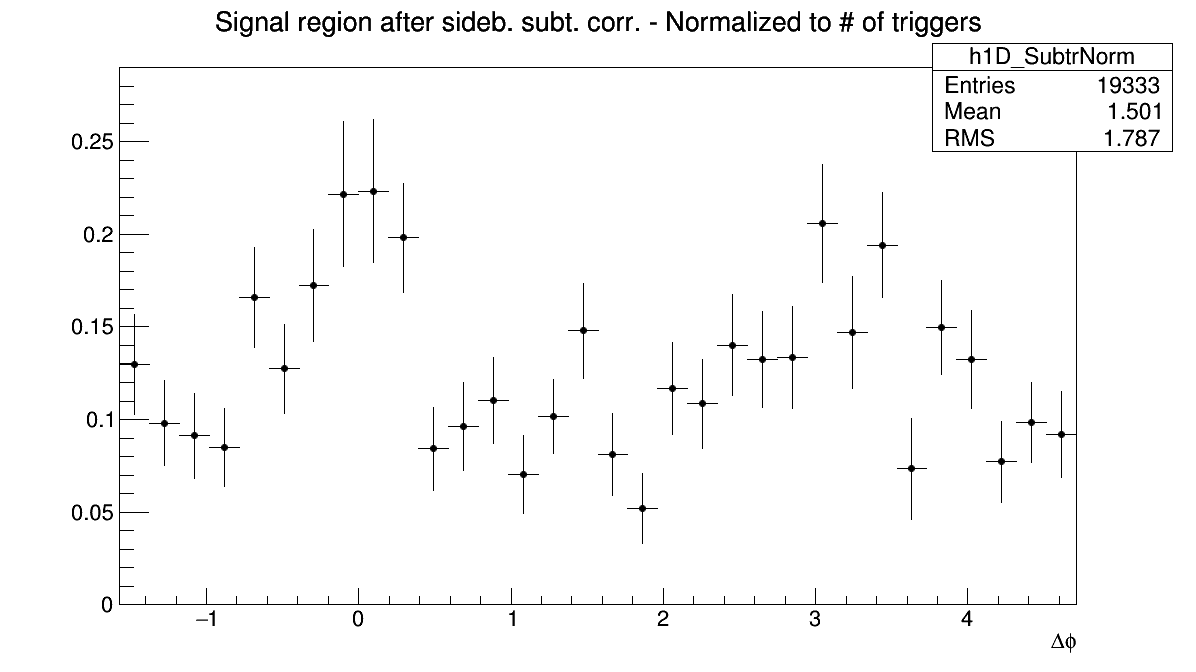
\includegraphics[width=0.31\linewidth, height=0.23\linewidth]{figures/DplusPlotsweff/AzimCorrDistr_Dplus_Canvas_PtIntBins5to7_PoolInt_thr2dotto3dot.png}}
{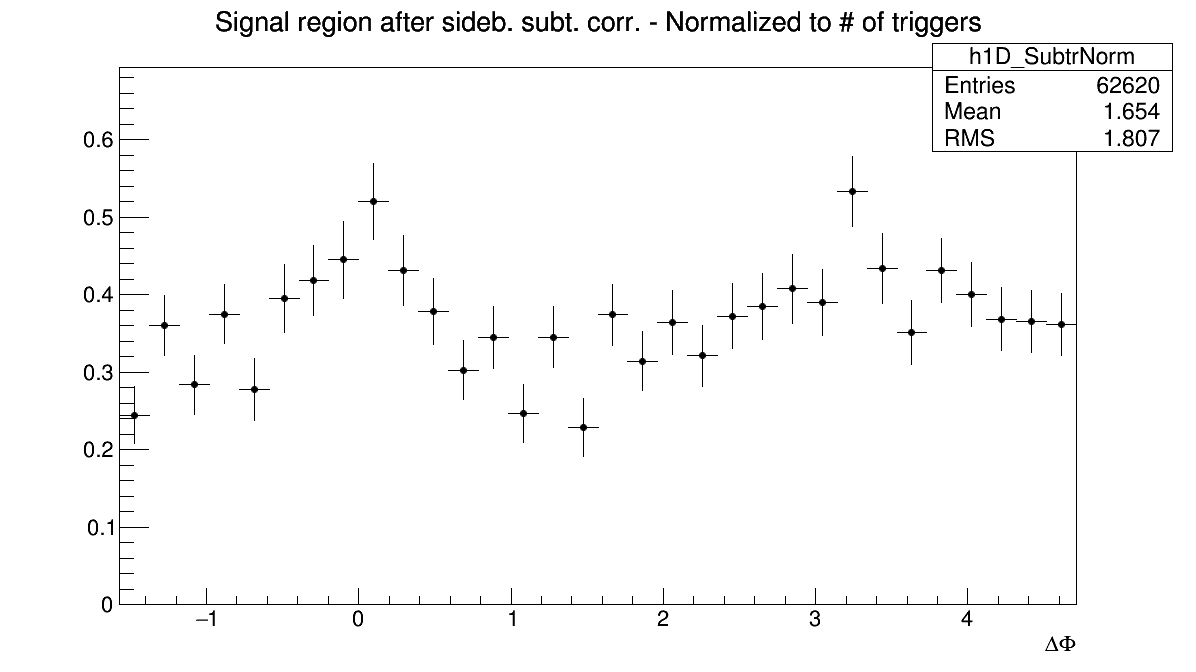
\includegraphics[width=0.31\linewidth, height=0.23\linewidth]{figures/Dstar_wEFF/AzimCorrDistr_Dstar_Canvas_PtIntBins4to6_PoolInt_thr2dotto3dot.png}}
% Pt>0.3 (High Pt)
{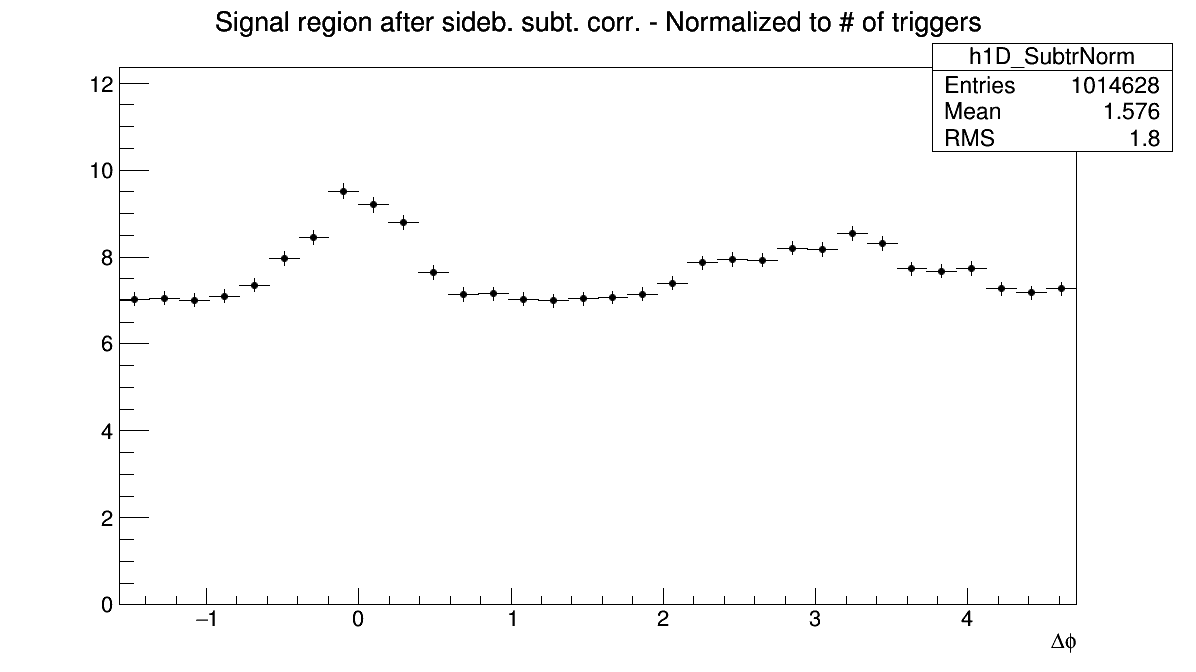
\includegraphics[width=0.31\linewidth, height=0.23\linewidth]{figures/Dzero/AzimCorrDistr_Dzero_Canvas_PtIntBins9to11_PoolInt_thrdot3to99dot.png}}
{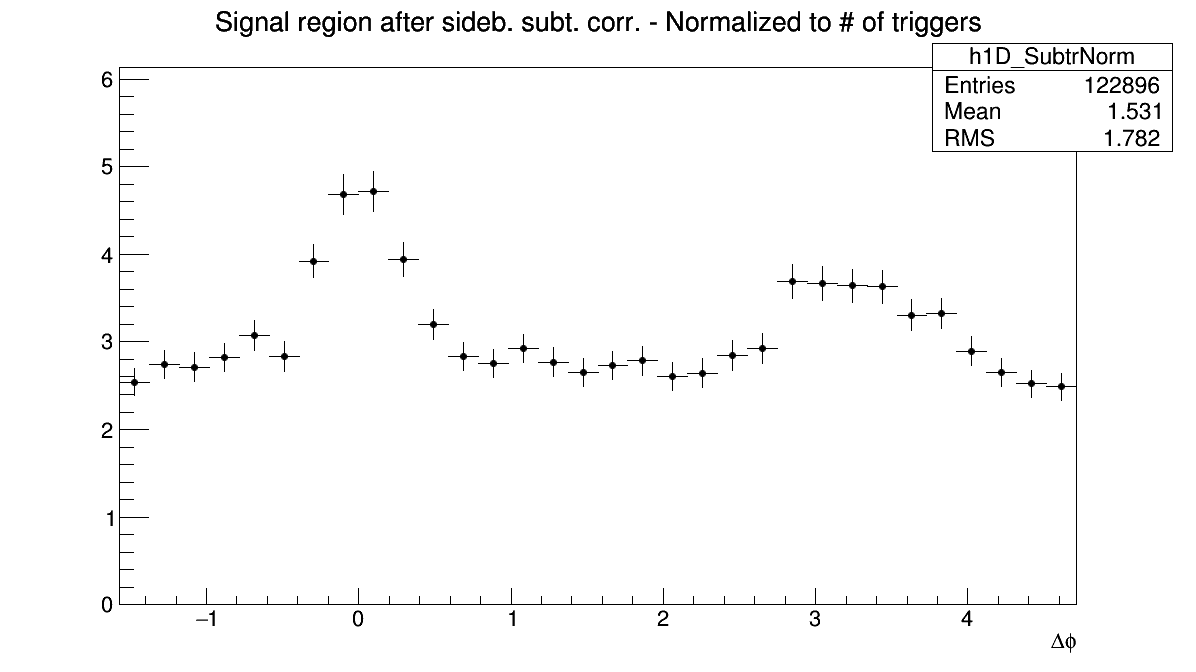
\includegraphics[width=0.31\linewidth, height=0.23\linewidth]{figures/DplusPlotsweff/AzimCorrDistr_Dplus_Canvas_PtIntBins8to12_PoolInt_thrdot3to99dot.png}}
{\includegraphics[width=0.31\linewidth, height=0.23\linewidth]{figures/Dstar_wEFF/AzimCorrDistr_Dstar_Canvas_PtIntBins7to9_PoolInt_thrdot3to99dot.png}}
% Pt>1.0 (High Pt)
{\includegraphics[width=0.31\linewidth, height=0.23\linewidth]{figures/Dzero/AzimCorrDistr_Dzero_Canvas_PtIntBins9to11_PoolInt_thr1dotto99dot.png}}
{\includegraphics[width=0.31\linewidth, height=0.23\linewidth]{figures/DplusPlotsweff/AzimCorrDistr_Dplus_Canvas_PtIntBins8to12_PoolInt_thr1dotto99dot.png}}
{\includegraphics[width=0.31\linewidth, height=0.23\linewidth]{figures/Dstar_wEFF/AzimCorrDistr_Dstar_Canvas_PtIntBins7to9_PoolInt_thr1dotto99dot.png}}
% Pt>2.0 (High Pt)
{\includegraphics[width=0.31\linewidth, height=0.23\linewidth]{figures/Dzero/AzimCorrDistr_Dzero_Canvas_PtIntBins9to11_PoolInt_thr2dotto99dot.png}}
{\includegraphics[width=0.31\linewidth, height=0.23\linewidth]{figures/DplusPlotsweff/AzimCorrDistr_Dplus_Canvas_PtIntBins8to12_PoolInt_thr2dotto99dot.png}}
{\includegraphics[width=0.31\linewidth, height=0.23\linewidth]{figures/Dstar_wEFF/AzimCorrDistr_Dstar_Canvas_PtIntBins7to9_PoolInt_thr2dotto99dot.png}}
% Pt>3.0 (High Pt)
{\includegraphics[width=0.31\linewidth, height=0.23\linewidth]{figures/Dzero/AzimCorrDistr_Dzero_Canvas_PtIntBins9to11_PoolInt_thr3dotto99dot.png}}
{\includegraphics[width=0.31\linewidth, height=0.23\linewidth]{figures/DplusPlotsweff/AzimCorrDistr_Dplus_Canvas_PtIntBins8to12_PoolInt_thr3dotto99dot.png}}
{\includegraphics[width=0.31\linewidth, height=0.23\linewidth]{figures/Dstar_wEFF/AzimCorrDistr_Dstar_Canvas_PtIntBins7to9_PoolInt_thr3dotto99dot.png}}
\end{figure}
\begin{figure}[!htbp]
\centering
% Pt>0.3-1.0 (High Pt)
{\includegraphics[width=0.31\linewidth, height=0.23\linewidth]{figures/Dzero/AzimCorrDistr_Dzero_Canvas_PtIntBins9to11_PoolInt_thrdot3to1dot.png}}
{\includegraphics[width=0.31\linewidth, height=0.23\linewidth]{figures/DplusPlotsweff/AzimCorrDistr_Dplus_Canvas_PtIntBins8to12_PoolInt_thrdot3to1dot.png}}
{\includegraphics[width=0.31\linewidth, height=0.23\linewidth]{figures/Dstar_wEFF/AzimCorrDistr_Dstar_Canvas_PtIntBins7to9_PoolInt_thrdot3to1dot.png}}
% Pt>1.0-2.0 (High Pt)
{\includegraphics[width=0.31\linewidth, height=0.23\linewidth]{figures/Dzero/AzimCorrDistr_Dzero_Canvas_PtIntBins9to11_PoolInt_thr1dotto2dot.png}}
{\includegraphics[width=0.31\linewidth, height=0.23\linewidth]{figures/DplusPlotsweff/AzimCorrDistr_Dplus_Canvas_PtIntBins8to12_PoolInt_thr1dotto2dot.png}}
{\includegraphics[width=0.31\linewidth, height=0.23\linewidth]{figures/Dstar_wEFF/AzimCorrDistr_Dstar_Canvas_PtIntBins7to9_PoolInt_thr1dotto2dot.png}}
% Pt>2.0-3.0 (High Pt)
{\includegraphics[width=0.31\linewidth, height=0.23\linewidth]{figures/Dzero/AzimCorrDistr_Dzero_Canvas_PtIntBins9to11_PoolInt_thr2dotto3dot.png}}
{\includegraphics[width=0.31\linewidth, height=0.23\linewidth]{figures/DplusPlotsweff/AzimCorrDistr_Dplus_Canvas_PtIntBins8to12_PoolInt_thr2dotto3dot.png}}
{\includegraphics[width=0.31\linewidth, height=0.23\linewidth]{figures/Dstar_wEFF/AzimCorrDistr_Dstar_Canvas_PtIntBins7to9_PoolInt_thr2dotto3dot.png}}

% Pt>0.3 (New Pt)
{\includegraphics[width=0.31\linewidth, height=0.23\linewidth]{figures/Dzero/AzimCorrDistr_Dzero_Canvas_PtIntBins12to12_PoolInt_thrdot3to99dot.png}}
{\includegraphics[width=0.31\linewidth, height=0.23\linewidth]{figures/DplusPlotsweff/AzimCorrDistr_Dplus_Canvas_PtIntBins13to13_PoolInt_thrdot3to99dot.png}}
{\includegraphics[width=0.31\linewidth, height=0.23\linewidth]{figures/Dstar_wEFF/AzimCorrDistr_Dstar_Canvas_PtIntBins10to10_PoolInt_thrdot3to99dot.png}}
% Pt>1.0 (New Pt)
{\includegraphics[width=0.31\linewidth, height=0.23\linewidth]{figures/Dzero/AzimCorrDistr_Dzero_Canvas_PtIntBins12to12_PoolInt_thr1dotto99dot.png}}
{\includegraphics[width=0.31\linewidth, height=0.23\linewidth]{figures/DplusPlotsweff/AzimCorrDistr_Dplus_Canvas_PtIntBins13to13_PoolInt_thr1dotto99dot.png}}
{\includegraphics[width=0.31\linewidth, height=0.23\linewidth]{figures/Dstar_wEFF/AzimCorrDistr_Dstar_Canvas_PtIntBins10to10_PoolInt_thr1dotto99dot.png}}
% Pt>2.0 (New Pt)
{\includegraphics[width=0.31\linewidth, height=0.23\linewidth]{figures/Dzero/AzimCorrDistr_Dzero_Canvas_PtIntBins12to12_PoolInt_thr2dotto99dot.png}}
{\includegraphics[width=0.31\linewidth, height=0.23\linewidth]{figures/DplusPlotsweff/AzimCorrDistr_Dplus_Canvas_PtIntBins13to13_PoolInt_thr2dotto99dot.png}}
{\includegraphics[width=0.31\linewidth, height=0.23\linewidth]{figures/Dstar_wEFF/AzimCorrDistr_Dstar_Canvas_PtIntBins10to10_PoolInt_thr2dotto99dot.png}}
\end{figure}
\begin{figure}[!htbp]
\centering
% Pt>3.0 (New Pt)
{\includegraphics[width=0.31\linewidth, height=0.23\linewidth]{figures/Dzero/AzimCorrDistr_Dzero_Canvas_PtIntBins12to12_PoolInt_thr3dotto99dot.png}}
{\includegraphics[width=0.31\linewidth, height=0.23\linewidth]{figures/DplusPlotsweff/AzimCorrDistr_Dplus_Canvas_PtIntBins13to13_PoolInt_thr3dotto99dot.png}}
{\includegraphics[width=0.31\linewidth, height=0.23\linewidth]{figures/Dstar_wEFF/AzimCorrDistr_Dstar_Canvas_PtIntBins10to10_PoolInt_thr3dotto99dot.png}}
% Pt>0.3-1.0 (New Pt)
{\includegraphics[width=0.31\linewidth, height=0.23\linewidth]{figures/Dzero/AzimCorrDistr_Dzero_Canvas_PtIntBins12to12_PoolInt_thrdot3to1dot.png}}
{\includegraphics[width=0.31\linewidth, height=0.23\linewidth]{figures/DplusPlotsweff/AzimCorrDistr_Dplus_Canvas_PtIntBins13to13_PoolInt_thrdot3to1dot.png}}
{\includegraphics[width=0.31\linewidth, height=0.23\linewidth]{figures/Dstar_wEFF/AzimCorrDistr_Dstar_Canvas_PtIntBins10to10_PoolInt_thrdot3to1dot.png}}
% Pt>1.0-2.0 (New Pt)
{\includegraphics[width=0.31\linewidth, height=0.23\linewidth]{figures/Dzero/AzimCorrDistr_Dzero_Canvas_PtIntBins12to12_PoolInt_thr1dotto2dot.png}}
{\includegraphics[width=0.31\linewidth, height=0.23\linewidth]{figures/DplusPlotsweff/AzimCorrDistr_Dplus_Canvas_PtIntBins13to13_PoolInt_thr1dotto2dot.png}}
{\includegraphics[width=0.31\linewidth, height=0.23\linewidth]{figures/Dstar_wEFF/AzimCorrDistr_Dstar_Canvas_PtIntBins10to10_PoolInt_thr1dotto2dot.png}}
% Pt>2.0-3.0 (New Pt)
{\includegraphics[width=0.31\linewidth, height=0.23\linewidth]{figures/Dzero/AzimCorrDistr_Dzero_Canvas_PtIntBins12to12_PoolInt_thr2dotto3dot.png}}
{\includegraphics[width=0.31\linewidth, height=0.23\linewidth]{figures/DplusPlotsweff/AzimCorrDistr_Dplus_Canvas_PtIntBins13to13_PoolInt_thr2dotto3dot.png}}
{\includegraphics[width=0.31\linewidth, height=0.23\linewidth]{figures/Dstar_wEFF/AzimCorrDistr_Dstar_Canvas_PtIntBins10to10_PoolInt_thr2dotto3dot.png}}
\caption{Corrected distribution of D-hadrons azimuthal correlations for the three species (apart from feed-down and purity), from analysis on the data sample, for the analyzed D-meson \textbf{(Column-Left: $D^0$, Column-Middle: $D^+$ and Column-Right: $\Dstar$)} and different associated tracks $p_\text{T}$ ranges (\textbf{Row 1-7:} $3 < D p_\text{T} < 5$ GeV$/c$, $ \ p_\text{T}~(Assoc)>$ 0.3, $>$1.0, $>$2.0, $>$3.0, 0.3-1.0, 1.0-2.0 and 2.0-3.0 GeV$/c$ respectively), (\textbf{Row 8-14:} $5 < D p_\text{T} < 8$ GeV$/c$, $ \ p_\text{T}~(Assoc)>$ 0.3, $>$1.0, $>$2.0, $>$3.0, 0.3-1.0, 1.0-2.0 and 2.0-3.0 GeV$/c$ respectively),(\textbf{Row 15-21:} $8 < D p_\text{T} < 16$ GeV$/c$, $ \ p_\text{T}~(Assoc)>$ 0.3, $>$1.0, $>$2.0, $>$3.0, 0.3-1.0, 1.0-2.0 and 2.0-3.0 GeV$/c$ respectively) and (\textbf{Row 22-28:} $16 < D p_\text{T} < 24$ GeV$/c$, $ \ p_\text{T}~(Assoc)>$ 0.3, $>$1.0, $>$2.0, $>$3.0, 0.3-1.0, 1.0-2.0 and 2.0-3.0 GeV$/c$ respectively) }.
\label{fig:DataD0DpDs}
\end{figure}

Figures~\ref{fig:Data_Res_D0DpDs},~\ref{fig:Data_Res_D0DpDs2},~\ref{fig:Data_Res_D0DpDs3},~\ref{fig:Data_Res_D0DpDs4} show the superimposed correlation distributions from the single-meson analyses (same plots as previous figure) for better visualize the agreeement among the different D-meson species results.

\clearpage
\newpage

\begin{figure}[!htbp]
\centering
%Superimposed Correlations
% D (Low Pt)
% Pt>0.3
{\includegraphics[width=0.48\linewidth]{figures/Averages/AzimCorrDistr_Canvas_PtIntBins3to5_PoolInt_thrdot3to99dot_Superimp.png}}
% Pt>0.3-1.0
{\includegraphics[width=0.48\linewidth]{figures/Averages/AzimCorrDistr_Canvas_PtIntBins3to5_PoolInt_thrdot3to1dot_Superimp.png}}
% Pt>1.0
{\includegraphics[width=0.48\linewidth]{figures/Averages/AzimCorrDistr_Canvas_PtIntBins3to5_PoolInt_thr1dotto99dot_Superimp.png}}
% Pt>1.0-2.0
{\includegraphics[width=0.48\linewidth]{figures/Averages/AzimCorrDistr_Canvas_PtIntBins3to5_PoolInt_thr1dotto2dot_Superimp.png}}
% Pt>2.0-3.0
{\includegraphics[width=0.48\linewidth]{figures/Averages/AzimCorrDistr_Canvas_PtIntBins3to5_PoolInt_thr2dotto3dot_Superimp.png}}
% Pt>3.0
{\includegraphics[width=0.48\linewidth]{figures/Averages/AzimCorrDistr_Canvas_PtIntBins3to5_PoolInt_thr3dotto99dot_Superimp.png}}
\caption{Superimposition of the corrected distribution of D-hadrons azimuthal correlations for the three species (apart from feed-down and purity), from analysis on the data sample, for the analyzed D-meson and different associated track $p_\text{T}$ ranges, and D-meson $\pt$ ranges (3-5 GeV/c on this page). \textbf{Panels from 1 to 6 of each page:} $ \ p_\text{T}~(Assoc)>$ 0.3, 0.3-1.0, $>$1.0, 1.0-2.0, 2.0-3.0 and $>$3.0 GeV$/c$}.
\label{fig:Data_Res_D0DpDs}
\end{figure}
\newpage
\begin{figure}
\centering
% Mid Pt
% Pt>0.3
{\includegraphics[width=0.48\linewidth]{figures/Averages/AzimCorrDistr_Canvas_PtIntBins5to8_PoolInt_thrdot3to99dot_Superimp.png}}
% Pt>0.3-1.0
{\includegraphics[width=0.48\linewidth]{figures/Averages/AzimCorrDistr_Canvas_PtIntBins5to8_PoolInt_thrdot3to1dot_Superimp.png}}
% Pt>1.0
{\includegraphics[width=0.48\linewidth]{figures/Averages/AzimCorrDistr_Canvas_PtIntBins5to8_PoolInt_thr1dotto99dot_Superimp.png}}
% Pt>1.0-2.0
{\includegraphics[width=0.48\linewidth]{figures/Averages/AzimCorrDistr_Canvas_PtIntBins5to8_PoolInt_thr1dotto2dot_Superimp.png}}
% Pt>2.0-3.0
{\includegraphics[width=0.48\linewidth]{figures/Averages/AzimCorrDistr_Canvas_PtIntBins5to8_PoolInt_thr2dotto3dot_Superimp.png}}
% Pt>3.0
{\includegraphics[width=0.48\linewidth]{figures/Averages/AzimCorrDistr_Canvas_PtIntBins5to8_PoolInt_thr3dotto99dot_Superimp.png}}
\caption{Superimposition of the corrected distribution of D-hadrons azimuthal correlations for the three species (apart from feed-down and purity), from analysis on the data sample, for the analyzed D-meson and different associated track $p_\text{T}$ ranges, and D-meson $\pt$ ranges (5-8 GeV/c on this page). \textbf{Panels from 1 to 6 of each page:} $ \ p_\text{T}~(Assoc)>$ 0.3, 0.3-1.0, $>$1.0, 1.0-2.0, 2.0-3.0 and $>$3.0 GeV$/c$}.
\label{fig:Data_Res_D0DpDs2}
% High Pt
\end{figure}
\newpage
\begin{figure}
\centering
% Pt>0.3
{\includegraphics[width=0.48\linewidth]{figures/Averages/AzimCorrDistr_Canvas_PtIntBins8to16_PoolInt_thrdot3to99dot_Superimp.png}}
% Pt>0.3-1.0
{\includegraphics[width=0.48\linewidth]{figures/Averages/AzimCorrDistr_Canvas_PtIntBins8to16_PoolInt_thrdot3to1dot_Superimp.png}}
% Pt>1.0
{\includegraphics[width=0.48\linewidth]{figures/Averages/AzimCorrDistr_Canvas_PtIntBins8to16_PoolInt_thr1dotto99dot_Superimp.png}}
% Pt>1.0-2.0
{\includegraphics[width=0.48\linewidth]{figures/Averages/AzimCorrDistr_Canvas_PtIntBins8to16_PoolInt_thr1dotto2dot_Superimp.png}}
% Pt>2.0-3.0
{\includegraphics[width=0.48\linewidth]{figures/Averages/AzimCorrDistr_Canvas_PtIntBins8to16_PoolInt_thr2dotto3dot_Superimp.png}}
% Pt>3.0
{\includegraphics[width=0.48\linewidth]{figures/Averages/AzimCorrDistr_Canvas_PtIntBins8to16_PoolInt_thr3dotto99dot_Superimp.png}}
\caption{Superimposition of the corrected distribution of D-hadrons azimuthal correlations for the three species (apart from feed-down and purity), from analysis on the data sample, for the analyzed D-meson and different associated track $p_\text{T}$ ranges, and D-meson $\pt$ ranges (8-16 GeV/c on this page). \textbf{Panels from 1 to 6 of each page:} $ \ p_\text{T}~(Assoc)>$ 0.3, 0.3-1.0, $>$1.0, 1.0-2.0, 2.0-3.0 and $>$3.0 GeV$/c$}.
\label{fig:Data_Res_D0DpDs3}
\end{figure}
\newpage
\begin{figure}
\centering
% New Pt
% Pt>0.3
{\includegraphics[width=0.48\linewidth]{figures/Averages/AzimCorrDistr_Canvas_PtIntBins16to24_PoolInt_thrdot3to99dot_Superimp.png}}
% Pt>0.3-1.0
{\includegraphics[width=0.48\linewidth]{figures/Averages/AzimCorrDistr_Canvas_PtIntBins16to24_PoolInt_thrdot3to1dot_Superimp.png}}
% Pt>1.0
{\includegraphics[width=0.48\linewidth]{figures/Averages/AzimCorrDistr_Canvas_PtIntBins16to24_PoolInt_thr1dotto99dot_Superimp.png}}
% Pt>1.0-2.0
{\includegraphics[width=0.48\linewidth]{figures/Averages/AzimCorrDistr_Canvas_PtIntBins16to24_PoolInt_thr1dotto2dot_Superimp.png}}
% Pt>2.0-3.0
{\includegraphics[width=0.48\linewidth]{figures/Averages/AzimCorrDistr_Canvas_PtIntBins16to24_PoolInt_thr2dotto3dot_Superimp.png}}
% Pt>3.0
{\includegraphics[width=0.48\linewidth]{figures/Averages/AzimCorrDistr_Canvas_PtIntBins16to24_PoolInt_thr3dotto99dot_Superimp.png}}
\caption{Superimposition of the corrected distribution of D-hadrons azimuthal correlations for the three species (apart from feed-down and purity), from analysis on the data sample, for the analyzed D-meson and different associated track $p_\text{T}$ ranges, and D-meson $\pt$ ranges (16-24 GeV/c on this page). \textbf{Panels from 1 to 6 of each page:} $ \ p_\text{T}~(Assoc)>$ 0.3, 0.3-1.0, $>$1.0, 1.0-2.0, 2.0-3.0 and $>$3.0 GeV$/c$}.
\label{fig:Data_Res_D0DpDs4}
\end{figure}

An agreement of the distributions from the three mesons within the uncertainties is found in all the kinematic ranges.

Despite being evaluated in the full $2\pi$ range, the range of final results was then reduced to $[0,\pi]$ radians, reflecting the points outside that range over the value of 0. This allowed to reduce the impact of statistical fluctuations on the data points (supposing equal statistics for a pair of symmetric bins, after the reflection the relative statistical uncertainty for the resulting bin is reduced by a factor $1/\sqrt{2}$).

%In figure \ref{fig:Data_CompareDZeroDStarDPhi}  a comparison of the $\Delta\varphi$ distributions  for $D^0$ (red points) and $D^{*+}$ (blue points) is shown. A very nice agreement is seen in with the $p_{T}$ ranges  $5 < D\ p_\text{T} < 8$ GeV/$c$ and $8 < D\ p_\text{T} < 16$ GeV/$c$. In the  $p_{T}$ range $3 < D\ p_\text{T} < 5$ GeV/$c$ there is a residual discrepancy on the baseline level, but the correlation shapes are compatible. This can be seen in  Fig.~\ref{fig:Data_CompareDZeroDStarYields}, where the comparison of the extracted Near Side yields and widths is shown \footnote{In this case, the pedestal is fixed to the average of the points in the region $-\pi/2<\Delta\varphi< -\pi/4$ and  $\pi/2<\Delta\varphi< \pi/4$.}.



\subsection{Average of $\Dzero$, $\Dplus$ and $\Dstar$ results}

%
%\begin{figure}
%\centering
%\includegraphics[width=.49\linewidth]{figures/xxxxxx} \\
%\includegraphics[width=.49\linewidth]{figures/xxxxxx}
%\caption{Comparison of $\Dzero$, $\Dstar$ azimuthal correlations and their average for  $5<\pt<8~\gev/c$
%and 8<$\pt$<16~$\gev/c$. Onnly the statistical uncertainties are shown. See text for details on the calculation of the averag and its uncertainty.
%}
%\label{fig:compareDzeroDstarAverage}
%\end{figure}
%
%
%
Given the compatibility within the uncertainties among the $\Dzero$, $\Dplus$ and $\Dstar$ azimuthal correlations, and since no large differences are visible in the correlation distributions observed in Monte Carlo simulations based on Pythia with Perugia0, 2010 and 2011 tunes\footnote{A slight near side hierarchy is present among the three meson results, with $\Dstar$ meson having a lower peak amplitude than $\Dzero$ and $\Dplus$. It was verified that this is induced by the presence of $\Dzero$ and $\Dplus$ mesons coming from $\Dstar$, the latter having on average a larger $p_T$ and coming, hence, on average, from a larger $p_T$ quark parton, which fragments in slightly more tracks in the near-side.}, it was possible to perform a weighted average (eq.~\ref{eqWeightedAv}) of the azimuthal correlation distributions of $\Dzero$, $\Dplus$ and $\Dstar$, in order to reduce the overall uncertainties.
Although some correlation between the mesons could be present (about the 30$\%$ of the $\Dzero$, and also part of the $\Dplus$, come from $\Dstar$ decays), the three selected D-meson samples can be treated as uncorrelated. The sum of the statistical uncertainties; the systematics uncertainty on S and B extraction and on background shape, are added in quadrature and the inverse of this sum was used as weight, $w_i$.
\begin{equation}
  \left \langle \frac{1}{N_{\rm D}}\frac{dN^{\rm assoc}}{d\pt} \right \rangle_{D mesons} =  \frac{\sum_{\rm i=meson}w_{i}\frac{1}{N_{\rm D}}\frac{dN^{\rm assoc}_{i}}{d\Delta\varphi}}{\sum_{\rm i=meson}w_{i}}\quad , w_{i}=\frac{1}{\sigma^{2}_{i, \rm stat}+\sigma^{2}_{i, \rm uncorr. syst.}}
\label{eqWeightedAv}
\end{equation}
The statistical uncertainty and the uncertainties on S and B extraction and on background shape (those used for the weights) on the average were then recalculated using the following formula:
\begin{equation}
  \sigma^{2}=\frac{1}{n_{\rm D}}\frac{\sum_{\rm i=meson}w_{i}\sigma^{2}_{i}}{\sum_{\rm i=meson}w_{i}}
\end{equation}
where $n_{\rm D}$ is the number of mesons considered in the average.
It can be observed that for $\sigma^{2}_{i}=1/w_{i}$ the formula coincides with the standard one giving the uncertainty on a weighted average.
The contribution to the average systematic uncertainty for those uncertainty sources not included in the weight definition, was evaluated via error propagation on the formula of the weighted average (\ref{eqWeightedAv}), resulting in equation (\ref{eqavsystuncor}) and (\ref{eqavsystcor}) for sources
considered uncorrelated and correlated among the mesons. In particular, the uncertainties on the associated track reconstruction efficiency, on the
contamination from secondary, on the feed-down subtraction, and that resulting from the Monte Carlo closure test were considered fully correlated among
the mesons, while those deriving from the yield extraction (included in the weight definition) and on the D meson reconstruction and selection efficiency were treated as uncorrelated.
\begin{eqnarray}
  \sigma^{2}=\frac{\sum_{\rm i=meson}w_{i}^{2}\sigma^{2}_{i}}{\left( \sum_{\rm i=meson}w_{i}\right)^{2}}  \label{eqavsystuncor}\\
  \sigma=\frac{\sum_{\rm i=meson}w_{i}\sigma_{i}}{ \sum_{\rm i=meson}w_{i}}   \label{eqavsystcor}
\end{eqnarray}
Figure~\ref{fig:DmesonAverage} shows the averages of the azimuthal correlation distributions of $\Dzero$, $\Dplus$ and $\Dstar$ and charged particles with $\pt>0.3~\gev/c$, 0.3$<\pt<1~\gev/c$, $\pt>1~\gev/c$, 1$<\pt<2~\gev/c$, 2$<\pt<3~\gev/c$, $\pt<3~\gev/c$ in the D meson $\pt$ ranges $3<\pt<5~\gev/c$, $5<\pt<8~\gev/c$, $8<\pt<16~\gev/c$ and $16<\pt<24~\gev/c$.
As expected, a rising trend of the height of the near-side peak with increasing D-meson $p_\mathrm{T}$ is observed, together with a decrease of the baseline level with increasing $p_\mathrm{T}$ of the associated tracks.
To further increase the statistical precision on the averaged correlation distributions, given the symmetry around 0 on the azimuthal axis, the distributions were reflected and shown in the range $[0,\pi]$. This reduces the statistical uncertainty on the poins by, approximately, a factor of $1/\sqrt{2}$.
\clearpage

\begin{figure}[!htbp]
\centering
%Marianna
%LowPt
%Pt>0.3
{\includegraphics[width=0.31\linewidth, height=0.23\linewidth]{figures/Averages/CanvaAndVariedHistoWeightedAverageDzeroDstarDplus_pPb_Pt3to5assocPtdot3to99dot.png}}
%Pt>1.0
{\includegraphics[width=0.31\linewidth, height=0.23\linewidth]{figures/Averages/CanvaAndVariedHistoWeightedAverageDzeroDstarDplus_pPb_Pt3to5assocPt1dotto99dot.png}}
%Pt>2.0
{\includegraphics[width=0.31\linewidth, height=0.23\linewidth]{figures/Averages/CanvaAndVariedHistoWeightedAverageDzeroDstarDplus_pPb_Pt3to5assocPt2dotto99dot.png}}
%Pt>3.0
{\includegraphics[width=0.31\linewidth, height=0.23\linewidth]{figures/Averages/CanvaAndVariedHistoWeightedAverageDzeroDstarDplus_pPb_Pt3to5assocPt3dotto99dot.png}}
%Pt>0.3-1.0
{\includegraphics[width=0.31\linewidth, height=0.23\linewidth]{figures/Averages/CanvaAndVariedHistoWeightedAverageDzeroDstarDplus_pPb_Pt3to5assocPtdot3to1dot.png}}
%Pt>1.0-2.0
{\includegraphics[width=0.31\linewidth, height=0.23\linewidth]{figures/Averages/CanvaAndVariedHistoWeightedAverageDzeroDstarDplus_pPb_Pt3to5assocPt1dotto2dot.png}}
%Pt>2.0-3.0
{\includegraphics[width=0.31\linewidth, height=0.23\linewidth]{figures/Averages/CanvaAndVariedHistoWeightedAverageDzeroDstarDplus_pPb_Pt3to5assocPt2dotto3dot.png}}
%MidPt
%Pt>0.3
{\includegraphics[width=0.31\linewidth, height=0.23\linewidth]{figures/Averages/CanvaAndVariedHistoWeightedAverageDzeroDstarDplus_pPb_Pt5to8assocPtdot3to99dot.png}}
%Pt>1.0
{\includegraphics[width=0.31\linewidth, height=0.23\linewidth]{figures/Averages/CanvaAndVariedHistoWeightedAverageDzeroDstarDplus_pPb_Pt5to8assocPt1dotto99dot.png}}
%Pt>2.0
{\includegraphics[width=0.31\linewidth, height=0.23\linewidth]{figures/Averages/CanvaAndVariedHistoWeightedAverageDzeroDstarDplus_pPb_Pt5to8assocPt2dotto99dot.png}}
%Pt>3.0
{\includegraphics[width=0.31\linewidth, height=0.23\linewidth]{figures/Averages/CanvaAndVariedHistoWeightedAverageDzeroDstarDplus_pPb_Pt5to8assocPt3dotto99dot.png}}
%Pt>0.3-1.0
{\includegraphics[width=0.31\linewidth, height=0.23\linewidth]{figures/Averages/CanvaAndVariedHistoWeightedAverageDzeroDstarDplus_pPb_Pt5to8assocPtdot3to1dot.png}}
%Pt>1.0-2.0
{\includegraphics[width=0.31\linewidth, height=0.23\linewidth]{figures/Averages/CanvaAndVariedHistoWeightedAverageDzeroDstarDplus_pPb_Pt5to8assocPt1dotto2dot.png}}
%Pt>2.0-3.0
{\includegraphics[width=0.31\linewidth, height=0.23\linewidth]{figures/Averages/CanvaAndVariedHistoWeightedAverageDzeroDstarDplus_pPb_Pt5to8assocPt2dotto3dot.png}}
%HighPt
%Pt>0.3
{\includegraphics[width=0.31\linewidth, height=0.23\linewidth]{figures/Averages/CanvaAndVariedHistoWeightedAverageDzeroDstarDplus_pPb_Pt8to16assocPtdot3to99dot.png}}
%Pt>1.0
{\includegraphics[width=0.31\linewidth, height=0.23\linewidth]{figures/Averages/CanvaAndVariedHistoWeightedAverageDzeroDstarDplus_pPb_Pt8to16assocPt1dotto99dot.png}}
%Pt>2.0
{\includegraphics[width=0.31\linewidth, height=0.23\linewidth]{figures/Averages/CanvaAndVariedHistoWeightedAverageDzeroDstarDplus_pPb_Pt8to16assocPt2dotto99dot.png}}
%Pt>3.0
{\includegraphics[width=0.31\linewidth, height=0.23\linewidth]{figures/Averages/CanvaAndVariedHistoWeightedAverageDzeroDstarDplus_pPb_Pt8to16assocPt3dotto99dot.png}}
\end{figure}
\begin{figure}[!htbp]
\centering
%Pt>0.3-1.0
{\includegraphics[width=0.31\linewidth, height=0.23\linewidth]{figures/Averages/CanvaAndVariedHistoWeightedAverageDzeroDstarDplus_pPb_Pt8to16assocPtdot3to1dot.png}}
%Pt>1.0-2.0
{\includegraphics[width=0.31\linewidth, height=0.23\linewidth]{figures/Averages/CanvaAndVariedHistoWeightedAverageDzeroDstarDplus_pPb_Pt8to16assocPt1dotto2dot.png}}
%Pt>2.0-3.0
{\includegraphics[width=0.31\linewidth, height=0.23\linewidth]{figures/Averages/CanvaAndVariedHistoWeightedAverageDzeroDstarDplus_pPb_Pt8to16assocPt2dotto3dot.png}}
%NewPt
%Pt>0.3
{\includegraphics[width=0.31\linewidth, height=0.23\linewidth]{figures/Averages/CanvaAndVariedHistoWeightedAverageDzeroDstarDplus_pPb_Pt16to24assocPtdot3to99dot.png}}
%Pt>1.0
{\includegraphics[width=0.31\linewidth, height=0.23\linewidth]{figures/Averages/CanvaAndVariedHistoWeightedAverageDzeroDstarDplus_pPb_Pt16to24assocPt1dotto99dot.png}}
%Pt>2.0
{\includegraphics[width=0.31\linewidth, height=0.23\linewidth]{figures/Averages/CanvaAndVariedHistoWeightedAverageDzeroDstarDplus_pPb_Pt16to24assocPt2dotto99dot.png}}
%Pt>3.0
{\includegraphics[width=0.31\linewidth, height=0.23\linewidth]{figures/Averages/CanvaAndVariedHistoWeightedAverageDzeroDstarDplus_pPb_Pt16to24assocPt3dotto99dot.png}}
%Pt>0.3-1.0
{\includegraphics[width=0.31\linewidth, height=0.23\linewidth]{figures/Averages/CanvaAndVariedHistoWeightedAverageDzeroDstarDplus_pPb_Pt16to24assocPtdot3to1dot.png}}
%Pt>1.0-2.0
{\includegraphics[width=0.31\linewidth, height=0.23\linewidth]{figures/Averages/CanvaAndVariedHistoWeightedAverageDzeroDstarDplus_pPb_Pt16to24assocPt1dotto2dot.png}}
%Pt>2.0-3.0
{\includegraphics[width=0.31\linewidth, height=0.23\linewidth]{figures/Averages/CanvaAndVariedHistoWeightedAverageDzeroDstarDplus_pPb_Pt16to24assocPt2dotto3dot.png}}
 \caption{Average of $\Dzero$, $\Dplus$ and $\Dstar$ azimuthal correlation distributions, in the D meson $\pt$ ranges $3<\pt<5~\gev/c$, $5<\pt<8~\gev/c$, $8<\pt<16~\gev/c$ and $16<\pt<24~\gev/c$, with associated tracks with $\pt>0.3~\gev/c$, $\pt>1~\gev/c$ and $0.3 < \pt < 1~\gev/c$.}
 \label{fig:DmesonAverage}
\end{figure}

The usage of weighted average requires, as an underlying assumption, identical results expected for different species (or, at least, compatible within the uncertainties). Anyway, it was also verified that the usage of the arithmetic average instead of the weighted average increases the uncertainties on the points, but produces a negligible shift of their central values.

%\begin{figure}
%\centering
%Marianna
%{\includegraphics[width=0.9\linewidth]{figures/WeightVsArithmAvg_pPb.png}}
%\caption{Comparison of weighted and arithmetic averages of $\Dzero$, $\Dplus$ and $\Dstar$-hadron correlations, in selected kinematic ranges.}
%\label{fig:CfrAveragesAppr}
%\end{figure}

\subsection{Fit observable $\pt$ trends and uncertainties}

%The extraction of the parameters (i.e. near side associated yield, near side width, and baseline) is performed using the strategy described above. The pedestal is calculated as the weighted average of the 8 points (for the full 2$\pi$ range plots) lying in the so-called "transverse region", i.e. the interval $\frac{\pi}{4}<|\Delta\varphi|<\frac{\pi}{2}$.

In order to extract quantitative and physical information from the data correlation patterns, the averaged D-h correlation distributions are fitted with two Gaussian functions (with means fixed at $\Delta\varphi$=0 and $\Delta\varphi$=$\pi$ values), plus a constant term (baseline). A periodicity condition is also applied to the fit function to obtain the same value at the bounds of 2$\pi$ range. The expression of the fit function is reported below (equation \ref{eq:fitfunction}):

%Added by Sandro
\begin{equation}
f\left(\Delta\varphi\right) = c + \frac{Y_{NS}}{\sqrt{2\pi}\sigma_{NS}}e^{-\frac{\left(\Delta\varphi-\mu_{NS}\right)^{2}}{2\sigma_{NS}^{2}}} + \frac{Y_{AS}}{\sqrt{2\pi}\sigma_{AS}}e^{-\frac{\left(\Delta\varphi-\mu_{AS}\right)^{2}}{2\sigma_{AS}^{2}}}
\label{eq:fitfunction}
\end{equation}

where baseline is calculated as the weighted average of the points lying in the so-called "transverse region", i.e. the interval $\frac{\pi}{4}<|\Delta\varphi|<\frac{\pi}{2}$.

An example of the results from the fit is shown in Figure~\ref{fig:ExFit}

\begin{figure}[h]
\centering
%\resizebox{0.7\textwidth}{!}
%Marianna
%Pt>2.0-3.0
{\includegraphics[width=0.99\linewidth, height=0.70\linewidth]{figures/FitOutput/cFitting_0_pthad1dotto99dot.png}}
%{\includegraphics[width=.75\linewidth]{figures/cFitOutput_NiceStyle_pPb_WeightedAverage_1_99.png}}
\caption{Example of fit to azimuthal correlation distributions and baseline estimation.}
 \label{fig:ExFit}
 \end{figure}

From the fit outcome, it is possible to retrieve the near-side and away-side yield and widths (integral and sigma of the Gaussian functions, respectively), as well as the baseline height of the correlation distribution. The near-side observables give information on the multiplicity and angular spread of the tracks from the fragmentation of the charm jet which gave birth to the D-meson trigger. At first order, instead, the away-side observables are related to the hadronization of the charm parton produced in the opposite direction (though the presence of NLO processes for charm production breaks the full validity of this assumption). The baseline value is a rough indicator of the underlying event multiplicity, though below the baseline level also charm and beauty-related pairs are contained (especially in cases of NLO production for the heavy quarks).

\begin{comment}
Figures (\ref{fig:dzerofinaldphifitted}), ( \ref{fig:dstarfinaldphifitted}) and ( \ref{fig:averagefinaldphifitted}) show the fitted correlation distributions of the $\Dzero$, $\Dstar$ and the average; the systematic boxes include only the uncorrelated systematics.


\begin{figure}
\centering
%\includegraphics[width=.49\linewidth]{figures/xxxxxx} \\
%\includegraphics[width=.49\linewidth]{figures/xxxxxx} \\
%\includegraphics[width=.49\linewidth]{figures/xxxxxx} \\
\caption{Final plot:  $\Dzero$ correlation, including only the uncorrelated systematics and the fitted function, with  $3 < D\ p_\text{T} < 5$ GeV/$c$, $5 < D\ p_\text{T} < 8$ GeV/$c$ and $8 < D\ p_\text{T} < 16$ GeV/$c$, while the associated tracks are selected with $p_{T}^{assoc}>0.3  GeV/c $.  }

\label{fig:dzerofinaldphifitted}
\end{figure}

\begin{figure}
\centering
%\includegraphics[width=.49\linewidth]{figures/xxxxxx} \\
%\includegraphics[width=.49\linewidth]{figures/xxxxxx} \\
%\includegraphics[width=.49\linewidth]{figures/xxxxxx} \\
\caption{Final plot:  $\Dstar$ correlation, including only the uncorrelated systematics and the fitted function, with  $3 < D\ p_\text{T} < 5$ GeV/$c$, $5 < D\ p_\text{T} < 8$ GeV/$c$ and $8 < D\ p_\text{T} < 16$ GeV/$c$, while the associated tracks are selected with $p_{T}^{assoc}>0.3  GeV/c $. The  plot with $3 < D\ p_\text{T} < 5$ GeV/c is not considered in the final plots, due to the discrepancy between $\Dzero$ and $\Dstar$ }

\label{fig:dstarfinaldphifitted}
\end{figure}

\begin{figure}
\centering
%\includegraphics[width=.49\linewidth]{figures/xxxxxx} \\
%\includegraphics[width=.49\linewidth]{figures/xxxxxx} \\
%\includegraphics[width=.49\linewidth]{figures/xxxxxx} \\
\caption{Final plot: average of $\Dzero$ and $\Dstar$ correlation, including only the uncorrelated systematics and the fitted function, with  $3 < D\ p_\text{T} < 5$ GeV/$c$, $5 < D\ p_\text{T} < 8$ GeV/$c$ and $8 < D\ p_\text{T} < 16$ GeV/$c$, while the associated tracks are selected with $p_{T}^{assoc}>0.3  GeV/c $. The  plot with $3 < D\ p_\text{T} < 5$ GeV/c is not considered in the final plots, due to the discrepancy between $\Dzero$ and $\Dstar$ }

\label{fig:averagefinaldphifitted}
\end{figure}

\end{comment}

The evaluation of the systematic uncertainties on the observables obtained from the fits is performed as follows:

\begin{itemize}
\item The fits are repeated by changing the range of the transverse region in which the baseline is evaluated. Alternate definitions of $\frac{\pi}{4}<|\Delta\varphi|<\frac{3\pi}{8}$, $\frac{3\pi}{8}<|\Delta\varphi|<\frac{\pi}{2}$ and $\frac{\pi}{4}<|\Delta\varphi|<\frac{5\pi}{8}$ are considered.
\item In addition, $\Delta\varphi$ correlation points are shifted to the upper and lower bounds of their uncorrelated systematic boxes, and refitted.
\item The fits are also repeated by moving the baseline value from its default value (i.e. with the default transverse region) on top and on bottom of its statistic uncertainty. This helps to account, though in a systematic uncertainty, for the statistical uncertainty on the baseline position (since in the fit the baseline is constrained, and its error is not propagated to the other observables).
\item The envelope between (i) the RMS of the relative variations of the parameters between the fit outcomes defined in the first two points, and (ii) the relative variations of the parameters from the fit outcomes defined in the third point, is considered as systematic uncertainty for the near-side and away-side widths.
\item For the estimation of the baseline and of the near-side and away-side yields, instead, the previous value is added in quadrature with the $\Delta\varphi$-correlated systematics in the correlation distributions, since these values are affected by a change in the global normalization of the distributions.
\item In addition, for all the fit observables, an additional fit variation is performed assuming, instead of a flat baseline, a v$_{2\Delta}$-like modulation, with the following v$_2$ values for the associated tracks (assuming $v_{2\Delta} = v_2({\rm h}) \cdot v_2({\rm D})$: 0.04 (0.3-1 GeV/c), 0.06 ($>$0.3 GeV/c), 0.08 (1-2 GeV/c), 0.09 ($>$1 GeV/c, 2-3 GeV/c), 0.1 ($>$3 GeV/c), on the basis of ATLAS preliminary results for heavy-flavour muons at 8 TeV; for the D-meson triggers the following v$_2$ values were instead assumed: 0.05 (3-5 GeV/c), 0.03 (5-8 GeV/c), 0.02 (8-24 GeV/c), on the basis of previous ALICE measurements in p-Pb collisions at 5 TeV \cite{ALICEv2ppb}. The difference of the fit observables with respect to the standard fits is taken as uncertainty. Due to its peculiarity, this systematic uncertainty is summed in quadrature with the others to obtain the total uncertainty, but is also shown separately in the figures.
\end{itemize}

\begin{equation}
\sigma^{syst} = \sqrt{\left(Max\left(\Delta par^{ped.mode},\Delta par^{\Delta\varphi point}\right)\right)^{2} + (\sigma_{Syst}^{corr})^{2}}
\end{equation}

\subsubsection{Results for near-side yield and width, away-side yield and width, and baseline}

Figures~\ref{fig:nearsideyieldAverage},~\ref{fig:nearsidesigmaAverage}, ~\ref{fig:awaysideyieldAverage},~\ref{fig:awaysidesigmaAverage} and~\ref{fig:baselineAverage} show the near-side associated yield, width (the sigma of the Gaussian part of the fit functions), away-side associated yield, width and the height of the baseline, for the average correlation distributions, in the kinematic ranges studied in the analysis, together with their statistical and systematic uncertainties. For each kinematic range, the correspondent plot showing the systematic uncertainty of the considered observable from the variation of the fit procedure is reported as well (which is the full systematic uncertainty for the widths).
Figures~\ref{fig:NSyieldTotalUnc},~\ref{fig:NSsigmaTotalUnc},~\ref{fig:ASyieldTotalUnc},~\ref{fig:ASsigmaTotalUnc} and~\ref{fig:baselineTotalUnc} show the full systematic uncertainties for near side yield and width, away side yield and width, and baseline, with the breakdown of fit variation, v$_2\Delta$ and $\Delta\varphi$ correlated systematic uncertainties.

\begin{figure}[!htbp]
\centering

%Marianna
%Pt>0.3
{\includegraphics[width=0.49\linewidth, height=0.33\linewidth]{figures/FitOutput/CanvasFinalTrendNSYield_pthaddot3to99dot.png}}
%Pt>1.0
{\includegraphics[width=0.49\linewidth, height=0.33\linewidth]{figures/FitOutput/CanvasFinalTrendNSYield_pthad1dotto99dot.png}}
%Pt>2.0
{\includegraphics[width=0.49\linewidth, height=0.33\linewidth]{figures/FitOutput/CanvasFinalTrendNSYield_pthad2dotto99dot.png}}
%Pt>3.0
{\includegraphics[width=0.49\linewidth, height=0.33\linewidth]{figures/FitOutput/CanvasFinalTrendNSYield_pthad3dotto99dot.png}}
%Pt>0.3-1.0
{\includegraphics[width=0.49\linewidth, height=0.33\linewidth]{figures/FitOutput/CanvasFinalTrendNSYield_pthaddot3to1dot.png}}
%Pt>1.0-2.0
{\includegraphics[width=0.49\linewidth, height=0.33\linewidth]{figures/FitOutput/CanvasFinalTrendNSYield_pthad1dotto2dot.png}}
%Pt>2.0-3.0
{\includegraphics[width=0.49\linewidth, height=0.33\linewidth]{figures/FitOutput/CanvasFinalTrendNSYield_pthad2dotto3dot.png}}
\end{figure}
\begin{figure}[!htbp]
\centering
%Pt>0.3
{\includegraphics[width=0.49\linewidth, height=0.33\linewidth]{figures/FitOutput/BaselineSystematicSourcesNSYield_pthaddot3to99dot.png}}
%Pt>1.0
{\includegraphics[width=0.49\linewidth, height=0.33\linewidth]{figures/FitOutput/BaselineSystematicSourcesNSYield_pthad1dotto99dot.png}}
%Pt>2.0
{\includegraphics[width=0.49\linewidth, height=0.33\linewidth]{figures/FitOutput/BaselineSystematicSourcesNSYield_pthad2dotto99dot.png}}
%Pt>3.0
{\includegraphics[width=0.49\linewidth, height=0.33\linewidth]{figures/FitOutput/BaselineSystematicSourcesNSYield_pthad3dotto99dot.png}}
%Pt>0.3-1.0
{\includegraphics[width=0.49\linewidth, height=0.33\linewidth]{figures/FitOutput/BaselineSystematicSourcesNSYield_pthaddot3to1dot.png}}
%Pt>1.0-2.0
{\includegraphics[width=0.49\linewidth, height=0.33\linewidth]{figures/FitOutput/BaselineSystematicSourcesNSYield_pthad1dotto2dot.png}}
%Pt>2.0-3.0
{\includegraphics[width=0.49\linewidth, height=0.33\linewidth]{figures/FitOutput/BaselineSystematicSourcesNSYield_pthad2dotto3dot.png}}
%\includegraphics[width=.49\linewidth]{figures/CanvasFinalTrendNSYield_pthad03to99.png}
%\includegraphics[width=.49\linewidth]{figures/BaselineSystematicSourcesNSYield_pthad03to99.png} \\
%\includegraphics[width=.49\linewidth]{figures/CanvasFinalTrendNSYield_pthad03to1.png}
%\includegraphics[width=.49\linewidth]{figures/BaselineSystematicSourcesNSYield_pthad03to1.png} \\
%\includegraphics[width=.49\linewidth]{figures/CanvasFinalTrendNSYield_pthad1to99.png}
%\includegraphics[width=.49\linewidth]{figures/BaselineSystematicSourcesNSYield_pthad1to99.png} \\
\caption{Top panels: near side yield $\pt$(D) trend for the D-meson average, extracted from fit to the azimuthal correlation distributions, for all the analyzed kinematic ranges of associated track $\pt$. Bottom panels: for each kinematic region the systematic uncertainties coming from the variation of the fit procedure are shown.}
\label{fig:nearsideyieldAverage}
\end{figure}

\begin{figure}[!htbp]
\centering

%Marianna
%Pt>0.3
{\includegraphics[width=0.49\linewidth, height=0.33\linewidth]{figures/FitOutput/CanvasFinalTrendNSSigma_pthaddot3to99dot.png}}
%Pt>1.0
{\includegraphics[width=0.49\linewidth, height=0.33\linewidth]{figures/FitOutput/CanvasFinalTrendNSSigma_pthad1dotto99dot.png}}
%Pt>2.0
{\includegraphics[width=0.49\linewidth, height=0.33\linewidth]{figures/FitOutput/CanvasFinalTrendNSSigma_pthad2dotto99dot.png}}
%Pt>3.0
{\includegraphics[width=0.49\linewidth, height=0.33\linewidth]{figures/FitOutput/CanvasFinalTrendNSSigma_pthad3dotto99dot.png}}
%Pt>0.3-1.0
{\includegraphics[width=0.49\linewidth, height=0.33\linewidth]{figures/FitOutput/CanvasFinalTrendNSSigma_pthaddot3to1dot.png}}
%Pt>1.0-2.0
{\includegraphics[width=0.49\linewidth, height=0.33\linewidth]{figures/FitOutput/CanvasFinalTrendNSSigma_pthad1dotto2dot.png}}
%Pt>2.0-3.0
{\includegraphics[width=0.49\linewidth, height=0.33\linewidth]{figures/FitOutput/CanvasFinalTrendNSSigma_pthad2dotto3dot.png}}
\end{figure}
\begin{figure}[!htbp]
\centering
%Pt>0.3
{\includegraphics[width=0.49\linewidth, height=0.33\linewidth]{figures/FitOutput/BaselineSystematicSourcesNSSigma_pthaddot3to99dot.png}}
%Pt>1.0
{\includegraphics[width=0.49\linewidth, height=0.33\linewidth]{figures/FitOutput/BaselineSystematicSourcesNSSigma_pthad1dotto99dot.png}}
%Pt>2.0
{\includegraphics[width=0.49\linewidth, height=0.33\linewidth]{figures/FitOutput/BaselineSystematicSourcesNSSigma_pthad2dotto99dot.png}}
%Pt>3.0
{\includegraphics[width=0.49\linewidth, height=0.33\linewidth]{figures/FitOutput/BaselineSystematicSourcesNSSigma_pthad3dotto99dot.png}}
%Pt>0.3-1.0
{\includegraphics[width=0.49\linewidth, height=0.33\linewidth]{figures/FitOutput/BaselineSystematicSourcesNSSigma_pthaddot3to1dot.png}}
%Pt>1.0-2.0
{\includegraphics[width=0.49\linewidth, height=0.33\linewidth]{figures/FitOutput/BaselineSystematicSourcesNSSigma_pthad1dotto2dot.png}}
%Pt>2.0-3.0
{\includegraphics[width=0.49\linewidth, height=0.33\linewidth]{figures/FitOutput/BaselineSystematicSourcesNSSigma_pthad2dotto3dot.png}}
%\includegraphics[width=.49\linewidth]{figures/CanvasFinalTrendNSSigma_pthad03to99.png}
%\includegraphics[width=.49\linewidth]{figures/BaselineSystematicSourcesNSSigma_pthad03to99.png} \\
%\includegraphics[width=.49\linewidth]{figures/CanvasFinalTrendNSSigma_pthad03to1.png}
%\includegraphics[width=.49\linewidth]{figures/BaselineSystematicSourcesNSSigma_pthad03to1.png} \\
%\includegraphics[width=.49\linewidth]{figures/CanvasFinalTrendNSSigma_pthad1to99.png}
%\includegraphics[width=.49\linewidth]{figures/BaselineSystematicSourcesNSSigma_pthad1to99.png} \\
\caption{Top panels: near side width $\pt$(D) trend for the D-meson average, extracted from fit to the azimuthal correlation distributions, for all the analyzed kinematic ranges of associated track $\pt$. Bottom panels:  for each kinematic region the systematic uncertainties coming from the variation of the fit procedure are shown.}
\label{fig:nearsidesigmaAverage}
\end{figure}

\begin{figure}[!htbp]
\centering

%Marianna
%Pt>0.3
{\includegraphics[width=0.49\linewidth, height=0.33\linewidth]{figures/FitOutput/CanvasFinalTrendASYield_pthaddot3to99dot.png}}
%Pt>1.0
{\includegraphics[width=0.49\linewidth, height=0.33\linewidth]{figures/FitOutput/CanvasFinalTrendASYield_pthad1dotto99dot.png}}
%Pt>2.0
{\includegraphics[width=0.49\linewidth, height=0.33\linewidth]{figures/FitOutput/CanvasFinalTrendASYield_pthad2dotto99dot.png}}
%Pt>3.0
{\includegraphics[width=0.49\linewidth, height=0.33\linewidth]{figures/FitOutput/CanvasFinalTrendASYield_pthad3dotto99dot.png}}
%Pt>0.3-1.0
{\includegraphics[width=0.49\linewidth, height=0.33\linewidth]{figures/FitOutput/CanvasFinalTrendASYield_pthaddot3to1dot.png}}
%Pt>1.0-2.0
{\includegraphics[width=0.49\linewidth, height=0.33\linewidth]{figures/FitOutput/CanvasFinalTrendASYield_pthad1dotto2dot.png}}
%Pt>2.0-3.0
{\includegraphics[width=0.49\linewidth, height=0.33\linewidth]{figures/FitOutput/CanvasFinalTrendASYield_pthad2dotto3dot.png}}
\end{figure}
\begin{figure}[!htbp]
\centering
%Pt>0.3
{\includegraphics[width=0.49\linewidth, height=0.33\linewidth]{figures/FitOutput/BaselineSystematicSourcesASYield_pthaddot3to99dot.png}}
%Pt>1.0
{\includegraphics[width=0.49\linewidth, height=0.33\linewidth]{figures/FitOutput/BaselineSystematicSourcesASYield_pthad1dotto99dot.png}}
%Pt>2.0
{\includegraphics[width=0.49\linewidth, height=0.33\linewidth]{figures/FitOutput/BaselineSystematicSourcesASYield_pthad2dotto99dot.png}}
%Pt>3.0
{\includegraphics[width=0.49\linewidth, height=0.33\linewidth]{figures/FitOutput/BaselineSystematicSourcesASYield_pthad3dotto99dot.png}}
%Pt>0.3-1.0
{\includegraphics[width=0.49\linewidth, height=0.33\linewidth]{figures/FitOutput/BaselineSystematicSourcesASYield_pthaddot3to1dot.png}}
%Pt>1.0-2.0
{\includegraphics[width=0.49\linewidth, height=0.33\linewidth]{figures/FitOutput/BaselineSystematicSourcesASYield_pthad1dotto2dot.png}}
%Pt>2.0-3.0
{\includegraphics[width=0.49\linewidth, height=0.33\linewidth]{figures/FitOutput/BaselineSystematicSourcesASYield_pthad2dotto3dot.png}}
%\includegraphics[width=.49\linewidth]{figures/CanvasFinalTrendNSYield_pthad03to99.png}
%\includegraphics[width=.49\linewidth]{figures/BaselineSystematicSourcesNSYield_pthad03to99.png} \\
%\includegraphics[width=.49\linewidth]{figures/CanvasFinalTrendNSYield_pthad03to1.png}
%\includegraphics[width=.49\linewidth]{figures/BaselineSystematicSourcesNSYield_pthad03to1.png} \\
%\includegraphics[width=.49\linewidth]{figures/CanvasFinalTrendNSYield_pthad1to99.png}
%\includegraphics[width=.49\linewidth]{figures/BaselineSystematicSourcesNSYield_pthad1to99.png} \\
\caption{Top panels: away side yield $\pt$(D) trend for the D-meson average, extracted from fit to the azimuthal correlation distributions, for all the analyzed kinematic ranges of associated track $\pt$. Bottom panels: for each kinematic region the systematic uncertainties coming from the variation of the fit procedure are shown.}
\label{fig:awaysideyieldAverage}
\end{figure}

\begin{figure}[!htbp]
\centering

%Marianna
%Pt>0.3
{\includegraphics[width=0.49\linewidth, height=0.33\linewidth]{figures/FitOutput/CanvasFinalTrendASSigma_pthaddot3to99dot.png}}
%Pt>1.0
{\includegraphics[width=0.49\linewidth, height=0.33\linewidth]{figures/FitOutput/CanvasFinalTrendASSigma_pthad1dotto99dot.png}}
%Pt>2.0
{\includegraphics[width=0.49\linewidth, height=0.33\linewidth]{figures/FitOutput/CanvasFinalTrendASSigma_pthad2dotto99dot.png}}
%Pt>3.0
{\includegraphics[width=0.49\linewidth, height=0.33\linewidth]{figures/FitOutput/CanvasFinalTrendASSigma_pthad3dotto99dot.png}}
%Pt>0.3-1.0
{\includegraphics[width=0.49\linewidth, height=0.33\linewidth]{figures/FitOutput/CanvasFinalTrendASSigma_pthaddot3to1dot.png}}
%Pt>1.0-2.0
{\includegraphics[width=0.49\linewidth, height=0.33\linewidth]{figures/FitOutput/CanvasFinalTrendASSigma_pthad1dotto2dot.png}}
%Pt>2.0-3.0
{\includegraphics[width=0.49\linewidth, height=0.33\linewidth]{figures/FitOutput/CanvasFinalTrendASSigma_pthad2dotto3dot.png}}
\end{figure}
\begin{figure}[!htbp]
\centering
%Pt>0.3
{\includegraphics[width=0.49\linewidth, height=0.33\linewidth]{figures/FitOutput/BaselineSystematicSourcesASSigma_pthaddot3to99dot.png}}
%Pt>1.0
{\includegraphics[width=0.49\linewidth, height=0.33\linewidth]{figures/FitOutput/BaselineSystematicSourcesASSigma_pthad1dotto99dot.png}}
%Pt>2.0
{\includegraphics[width=0.49\linewidth, height=0.33\linewidth]{figures/FitOutput/BaselineSystematicSourcesASSigma_pthad2dotto99dot.png}}
%Pt>3.0
{\includegraphics[width=0.49\linewidth, height=0.33\linewidth]{figures/FitOutput/BaselineSystematicSourcesASSigma_pthad3dotto99dot.png}}
%Pt>0.3-1.0
{\includegraphics[width=0.49\linewidth, height=0.33\linewidth]{figures/FitOutput/BaselineSystematicSourcesASSigma_pthaddot3to1dot.png}}
%Pt>1.0-2.0
{\includegraphics[width=0.49\linewidth, height=0.33\linewidth]{figures/FitOutput/BaselineSystematicSourcesASSigma_pthad1dotto2dot.png}}
%Pt>2.0-3.0
{\includegraphics[width=0.49\linewidth, height=0.33\linewidth]{figures/FitOutput/BaselineSystematicSourcesASSigma_pthad2dotto3dot.png}}

%\includegraphics[width=.49\linewidth]{figures/CanvasFinalTrendNSYield_pthad03to99.png}
%\includegraphics[width=.49\linewidth]{figures/BaselineSystematicSourcesNSYield_pthad03to99.png} \\
%\includegraphics[width=.49\linewidth]{figures/CanvasFinalTrendNSYield_pthad03to1.png}
%\includegraphics[width=.49\linewidth]{figures/BaselineSystematicSourcesNSYield_pthad03to1.png} \\
%\includegraphics[width=.49\linewidth]{figures/CanvasFinalTrendNSYield_pthad1to99.png}
%\includegraphics[width=.49\linewidth]{figures/BaselineSystematicSourcesNSYield_pthad1to99.png} \\
\caption{Top panels: away side width $\pt$(D) trend for the D-meson average, extracted from fit to the azimuthal correlation distributions, for all the analyzed kinematic ranges of associated track $\pt$. Bottom panels: for each kinematic region the systematic uncertainties coming from the variation of the fit procedure are shown.}
\label{fig:awaysidesigmaAverage}
\end{figure}

\begin{figure}[!htbp]
\centering
%Marianna
%Pt>0.3
{\includegraphics[width=0.49\linewidth, height=0.33\linewidth]{figures/FitOutput/CanvasFinalTrendPedestal_pthaddot3to99dot.png}}
%Pt>1.0
{\includegraphics[width=0.49\linewidth, height=0.33\linewidth]{figures/FitOutput/CanvasFinalTrendPedestal_pthad1dotto99dot.png}}
%Pt>2.0
{\includegraphics[width=0.49\linewidth, height=0.33\linewidth]{figures/FitOutput/CanvasFinalTrendPedestal_pthad2dotto99dot.png}}
%Pt>3.0
{\includegraphics[width=0.49\linewidth, height=0.33\linewidth]{figures/FitOutput/CanvasFinalTrendPedestal_pthad3dotto99dot.png}}
%Pt>0.3-1.0
{\includegraphics[width=0.49\linewidth, height=0.33\linewidth]{figures/FitOutput/CanvasFinalTrendPedestal_pthaddot3to1dot.png}}
%Pt>1.0-2.0
{\includegraphics[width=0.49\linewidth, height=0.33\linewidth]{figures/FitOutput/CanvasFinalTrendPedestal_pthad1dotto2dot.png}}
%Pt>2.0-3.0
{\includegraphics[width=0.49\linewidth, height=0.33\linewidth]{figures/FitOutput/CanvasFinalTrendPedestal_pthad2dotto3dot.png}}
\end{figure}

\begin{figure}[!htbp]
\centering
%Marianna
%Pt>0.3
{\includegraphics[width=0.49\linewidth, height=0.33\linewidth]{figures/FitOutput/BaselineSystematicSourcesPedestal_pthaddot3to99dot.png}}
%Pt>1.0
{\includegraphics[width=0.49\linewidth, height=0.33\linewidth]{figures/FitOutput/BaselineSystematicSourcesPedestal_pthad1dotto99dot.png}}
%Pt>2.0
{\includegraphics[width=0.49\linewidth, height=0.33\linewidth]{figures/FitOutput/BaselineSystematicSourcesPedestal_pthad2dotto99dot.png}}
%Pt>3.0
{\includegraphics[width=0.49\linewidth, height=0.33\linewidth]{figures/FitOutput/BaselineSystematicSourcesPedestal_pthad3dotto99dot.png}}
%Pt>0.3-1.0
{\includegraphics[width=0.49\linewidth, height=0.33\linewidth]{figures/FitOutput/BaselineSystematicSourcesPedestal_pthaddot3to1dot.png}}
%Pt>1.0-2.0
{\includegraphics[width=0.49\linewidth, height=0.33\linewidth]{figures/FitOutput/BaselineSystematicSourcesPedestal_pthad1dotto2dot.png}}
%Pt>2.0-3.0
{\includegraphics[width=0.49\linewidth, height=0.33\linewidth]{figures/FitOutput/BaselineSystematicSourcesPedestal_pthad2dotto3dot.png}}
%\includegraphics[width=.49\linewidth]{figures/CanvasFinalTrendPedestal_pthad03to99.png}
%\includegraphics[width=.49\linewidth]{figures/BaselineSystematicSourcesPedestal_pthad03to99.png} \\
%\includegraphics[width=.49\linewidth]{figures/CanvasFinalTrendPedestal_pthad03to1.png}
%\includegraphics[width=.49\linewidth]{figures/BaselineSystematicSourcesPedestal_pthad03to1.png} \\
%\includegraphics[width=.49\linewidth]{figures/CanvasFinalTrendPedestal_pthad1to99.png}
%\includegraphics[width=.49\linewidth]{figures/BaselineSystematicSourcesPedestal_pthad1to99.png} \\
\caption{Top panels: baseline height trend for the D-meson average, extracted from fit to the azimuthal correlation distributions, for all the analyzed kinematic ranges of associated track $\pt$. Bottom panels: for each kinematic region the systematic uncertainties coming from the variation of the fit procedure are shown.}
\label{fig:baselineAverage}
\end{figure}

\begin{figure}[!htbp]
\centering

%Marianna
%Pt>0.3
{\includegraphics[width=0.49\linewidth, height=0.33\linewidth]{figures/FitOutput/TotalSystematicSourcesNSYield_pthaddot3to99dot.png}}
%Pt>1.0
{\includegraphics[width=0.49\linewidth, height=0.33\linewidth]{figures/FitOutput/TotalSystematicSourcesNSYield_pthad1dotto99dot.png}}
%Pt>2.0
{\includegraphics[width=0.49\linewidth, height=0.33\linewidth]{figures/FitOutput/TotalSystematicSourcesNSYield_pthad2dotto99dot.png}}
%Pt>3.0
{\includegraphics[width=0.49\linewidth, height=0.33\linewidth]{figures/FitOutput/TotalSystematicSourcesNSYield_pthad3dotto99dot.png}}
%Pt>0.3-1.0
{\includegraphics[width=0.49\linewidth, height=0.33\linewidth]{figures/FitOutput/TotalSystematicSourcesNSYield_pthaddot3to1dot.png}}
%Pt>1.0-2.0
{\includegraphics[width=0.49\linewidth, height=0.33\linewidth]{figures/FitOutput/TotalSystematicSourcesNSYield_pthad1dotto2dot.png}}
%Pt>2.0-3.0
{\includegraphics[width=0.49\linewidth, height=0.33\linewidth]{figures/FitOutput/TotalSystematicSourcesNSYield_pthad2dotto3dot.png}}
%\includegraphics[width=.49\linewidth]{figures/CanvasFinalTrendNSYield_pthad03to99.png}
%\includegraphics[width=.49\linewidth]{figures/BaselineSystematicSourcesNSYield_pthad03to99.png} \\
%\includegraphics[width=.49\linewidth]{figures/CanvasFinalTrendNSYield_pthad03to1.png}
%\includegraphics[width=.49\linewidth]{figures/BaselineSystematicSourcesNSYield_pthad03to1.png} \\
%\includegraphics[width=.49\linewidth]{figures/CanvasFinalTrendNSYield_pthad1to99.png}
%\includegraphics[width=.49\linewidth]{figures/BaselineSystematicSourcesNSYield_pthad1to99.png} \\
\caption{Total systematic uncertainty, and its components, for near-side yields in the different kinematic ranges analyzed}
\label{fig:NSyieldTotalUnc}
\end{figure}

\begin{figure}[!htbp]
\centering

%Marianna
%Pt>0.3
{\includegraphics[width=0.49\linewidth, height=0.33\linewidth]{figures/FitOutput/TotalSystematicSourcesNSSigma_pthaddot3to99dot.png}}
%Pt>1.0
{\includegraphics[width=0.49\linewidth, height=0.33\linewidth]{figures/FitOutput/TotalSystematicSourcesNSSigma_pthad1dotto99dot.png}}
%Pt>2.0
{\includegraphics[width=0.49\linewidth, height=0.33\linewidth]{figures/FitOutput/TotalSystematicSourcesNSSigma_pthad2dotto99dot.png}}
%Pt>3.0
{\includegraphics[width=0.49\linewidth, height=0.33\linewidth]{figures/FitOutput/TotalSystematicSourcesNSSigma_pthad3dotto99dot.png}}
%Pt>0.3-1.0
{\includegraphics[width=0.49\linewidth, height=0.33\linewidth]{figures/FitOutput/TotalSystematicSourcesNSSigma_pthaddot3to1dot.png}}
%Pt>1.0-2.0
{\includegraphics[width=0.49\linewidth, height=0.33\linewidth]{figures/FitOutput/TotalSystematicSourcesNSSigma_pthad1dotto2dot.png}}
%Pt>2.0-3.0
{\includegraphics[width=0.49\linewidth, height=0.33\linewidth]{figures/FitOutput/TotalSystematicSourcesNSSigma_pthad2dotto3dot.png}}
%\includegraphics[width=.49\linewidth]{figures/CanvasFinalTrendNSYield_pthad03to99.png}
%\includegraphics[width=.49\linewidth]{figures/BaselineSystematicSourcesNSYield_pthad03to99.png} \\
%\includegraphics[width=.49\linewidth]{figures/CanvasFinalTrendNSYield_pthad03to1.png}
%\includegraphics[width=.49\linewidth]{figures/BaselineSystematicSourcesNSYield_pthad03to1.png} \\
%\includegraphics[width=.49\linewidth]{figures/CanvasFinalTrendNSYield_pthad1to99.png}
%\includegraphics[width=.49\linewidth]{figures/BaselineSystematicSourcesNSYield_pthad1to99.png} \\
\caption{Total systematic uncertainty, and its components, for near-side sigma in the different kinematic ranges analyzed}
\label{fig:NSsigmaTotalUnc}
\end{figure}

\begin{figure}[!htbp]
\centering

%Marianna
%Pt>0.3
{\includegraphics[width=0.49\linewidth, height=0.33\linewidth]{figures/FitOutput/TotalSystematicSourcesASYield_pthaddot3to99dot.png}}
%Pt>1.0
{\includegraphics[width=0.49\linewidth, height=0.33\linewidth]{figures/FitOutput/TotalSystematicSourcesASYield_pthad1dotto99dot.png}}
%Pt>2.0
{\includegraphics[width=0.49\linewidth, height=0.33\linewidth]{figures/FitOutput/TotalSystematicSourcesASYield_pthad2dotto99dot.png}}
%Pt>3.0
{\includegraphics[width=0.49\linewidth, height=0.33\linewidth]{figures/FitOutput/TotalSystematicSourcesASYield_pthad3dotto99dot.png}}
%Pt>0.3-1.0
{\includegraphics[width=0.49\linewidth, height=0.33\linewidth]{figures/FitOutput/TotalSystematicSourcesASYield_pthaddot3to1dot.png}}
%Pt>1.0-2.0
{\includegraphics[width=0.49\linewidth, height=0.33\linewidth]{figures/FitOutput/TotalSystematicSourcesASYield_pthad1dotto2dot.png}}
%Pt>2.0-3.0
{\includegraphics[width=0.49\linewidth, height=0.33\linewidth]{figures/FitOutput/TotalSystematicSourcesASYield_pthad2dotto3dot.png}}
%\includegraphics[width=.49\linewidth]{figures/CanvasFinalTrendNSYield_pthad03to99.png}
%\includegraphics[width=.49\linewidth]{figures/BaselineSystematicSourcesNSYield_pthad03to99.png} \\
%\includegraphics[width=.49\linewidth]{figures/CanvasFinalTrendNSYield_pthad03to1.png}
%\includegraphics[width=.49\linewidth]{figures/BaselineSystematicSourcesNSYield_pthad03to1.png} \\
%\includegraphics[width=.49\linewidth]{figures/CanvasFinalTrendNSYield_pthad1to99.png}
%\includegraphics[width=.49\linewidth]{figures/BaselineSystematicSourcesNSYield_pthad1to99.png} \\
\caption{Total systematic uncertainty, and its components, for away-side yields in the different kinematic ranges analyzed}
\label{fig:ASyieldTotalUnc}
\end{figure}

\begin{figure}[!htbp]
\centering

%Marianna
%Pt>0.3
{\includegraphics[width=0.49\linewidth, height=0.33\linewidth]{figures/FitOutput/TotalSystematicSourcesASSigma_pthaddot3to99dot.png}}
%Pt>1.0
{\includegraphics[width=0.49\linewidth, height=0.33\linewidth]{figures/FitOutput/TotalSystematicSourcesASSigma_pthad1dotto99dot.png}}
%Pt>2.0
{\includegraphics[width=0.49\linewidth, height=0.33\linewidth]{figures/FitOutput/TotalSystematicSourcesASSigma_pthad2dotto99dot.png}}
%Pt>3.0
{\includegraphics[width=0.49\linewidth, height=0.33\linewidth]{figures/FitOutput/TotalSystematicSourcesASSigma_pthad3dotto99dot.png}}
%Pt>0.3-1.0
{\includegraphics[width=0.49\linewidth, height=0.33\linewidth]{figures/FitOutput/TotalSystematicSourcesASSigma_pthaddot3to1dot.png}}
%Pt>1.0-2.0
{\includegraphics[width=0.49\linewidth, height=0.33\linewidth]{figures/FitOutput/TotalSystematicSourcesASSigma_pthad1dotto2dot.png}}
%Pt>2.0-3.0
{\includegraphics[width=0.49\linewidth, height=0.33\linewidth]{figures/FitOutput/TotalSystematicSourcesASSigma_pthad2dotto3dot.png}}
%\includegraphics[width=.49\linewidth]{figures/CanvasFinalTrendNSYield_pthad03to99.png}
%\includegraphics[width=.49\linewidth]{figures/BaselineSystematicSourcesNSYield_pthad03to99.png} \\
%\includegraphics[width=.49\linewidth]{figures/CanvasFinalTrendNSYield_pthad03to1.png}
%\includegraphics[width=.49\linewidth]{figures/BaselineSystematicSourcesNSYield_pthad03to1.png} \\
%\includegraphics[width=.49\linewidth]{figures/CanvasFinalTrendNSYield_pthad1to99.png}
%\includegraphics[width=.49\linewidth]{figures/BaselineSystematicSourcesNSYield_pthad1to99.png} \\
\caption{Total systematic uncertainty, and its components, for away-side sigma in the different kinematic ranges analyzed}
\label{fig:ASsigmaTotalUnc}
\end{figure}


\begin{figure}[!htbp]
\centering
%Marianna
\centering
%Pt>0.3
{\includegraphics[width=0.49\linewidth, height=0.33\linewidth]{figures/FitOutput/TotalSystematicSourcesPedestal_pthaddot3to99dot.png}}
%Pt>1.0
{\includegraphics[width=0.49\linewidth, height=0.33\linewidth]{figures/FitOutput/TotalSystematicSourcesPedestal_pthad1dotto99dot.png}}
%Pt>2.0
{\includegraphics[width=0.49\linewidth, height=0.33\linewidth]{figures/FitOutput/TotalSystematicSourcesPedestal_pthad2dotto99dot.png}}
%Pt>3.0
{\includegraphics[width=0.49\linewidth, height=0.33\linewidth]{figures/FitOutput/TotalSystematicSourcesPedestal_pthad3dotto99dot.png}}
%Pt>0.3-1.0
{\includegraphics[width=0.49\linewidth, height=0.33\linewidth]{figures/FitOutput/TotalSystematicSourcesPedestal_pthaddot3to1dot.png}}
%Pt>1.0-2.0
{\includegraphics[width=0.49\linewidth, height=0.33\linewidth]{figures/FitOutput/TotalSystematicSourcesPedestal_pthad1dotto2dot.png}}
%Pt>2.0-3.0
{\includegraphics[width=0.49\linewidth, height=0.33\linewidth]{figures/FitOutput/TotalSystematicSourcesPedestal_pthad2dotto3dot.png}}
%\includegraphics[width=.49\linewidth]{figures/CanvasFinalTrendPedestal_pthad03to99.png}
%\includegraphics[width=.49\linewidth]{figures/BaselineSystematicSourcesPedestal_pthad03to99.png} \\
%\includegraphics[width=.49\linewidth]{figures/CanvasFinalTrendPedestal_pthad03to1.png}
%\includegraphics[width=.49\linewidth]{figures/BaselineSystematicSourcesPedestal_pthad03to1.png} \\
%\includegraphics[width=.49\linewidth]{figures/CanvasFinalTrendPedestal_pthad1to99.png}
%\includegraphics[width=.49\linewidth]{figures/BaselineSystematicSourcesPedestal_pthad1to99.png} \\
\caption{Total systematic uncertainty, and its components, for baseline heights in the different kinematic ranges analyzed.}
\label{fig:baselineTotalUnc}
\end{figure}

\begin{comment}
\subsubsection{Comparisons pp and p--Pb}

Figure~\ref{fig:pp-pPb} shows the average of $\Dzero$, $\Dplus$ and $\Dstar$ azimuthal correlations for pp and pPb for two different ranges of trigger and associated $p_\mathrm{T}$. Compatibility within uncertainties between the two collision systems is found for all the common kinematic ranges analyzed. In Figure~\ref{fig:pp-pPb_Fit}, the comparison of the observables extracted from the fits (near-side yield, width and baseline height) is also presented.

\begin{figure}
\centering
%Marianna
%\includegraphics[width=.45\linewidth]{figures/plotComparison_WeightedAverage_pp_pPb_58_03to99.eps}
%\includegraphics[width=.45\linewidth]{figures/plotComparison_WeightedAverage_pp_pPb_816_03to99.eps} \\
%\includegraphics[width=.45\linewidth]{figures/plotComparison_WeightedAverage_pp_pPb_58_03to1.eps}
%\includegraphics[width=.45\linewidth]{figures/plotComparison_WeightedAverage_pp_pPb_816_03to1.eps} \\
%\includegraphics[width=.45\linewidth]{figures/plotComparison_WeightedAverage_pp_pPb_58_1to99.eps}
%\includegraphics[width=.45\linewidth]{figures/plotComparison_WeightedAverage_pp_pPb_816_1to99.eps} \\
\caption{Average of $\Dzero$, $\Dplus$ and $\Dstar$ azimuthal correlations in pp (red) and p-Pb (blue) with D meson $\pt$ in the range $5<\pt<8~\gev/c$ and $8<\pt<16~\gev/c$, for the three regions of associated track transverse momentum.}
\label{fig:pp-pPb}
\end{figure}

\begin{figure}
\centering
\includegraphics[width=.95\linewidth]{figures/Cfr_pp_Pb_FitPars.png}
\caption{Fit parameters for the average of $\Dzero$, $\Dplus$ and $\Dstar$ azimuthal correlations in pp (red) and p-Pb (black) with D meson $\pt$ in the range $5<\pt<8~\gev/c$ and $8<\pt<16~\gev/c$, for the three regions of associated track transverse momentum.}
\label{fig:pp-pPb_Fit}
\end{figure}

\subsubsection{Comparisons p--Pb and Pythia}
Figure \ref{fig:pp-pPb} shows the average of $\Dzero$, $\Dplus$ and $\Dstar$ azimuthal correlations for pPb for two different ranges of trigger and associated $p_\mathrm{T}$, compared to different Pythia tunes at the same collision energy (Pythia 8 tune Perugia-0, Pythia 8 tune 2011). A substantial agreement within the uncertainties is observed.%, though all the simulations underestimate the near side, especially for the highest D-meson $p_{t}$ range.

\begin{figure}[h]
\centering
%Marianna
%\includegraphics[width=.45\linewidth]{figures/plotComparison_WeightedAverage_pPb_MC_58_03to99.png}
%\includegraphics[width=.45\linewidth]{figures/plotComparison_WeightedAverage_pPb_MC_816_03to99.png} \\
%\includegraphics[width=.45\linewidth]{figures/plotComparison_WeightedAverage_pPb_MC_58_03to1.png}
%\includegraphics[width=.45\linewidth]{figures/plotComparison_WeightedAverage_pPb_MC_816_03to1.png} \\
%\includegraphics[width=.45\linewidth]{figures/plotComparison_WeightedAverage_pPb_MC_58_1to99.png}
%\includegraphics[width=.45\linewidth]{figures/plotComparison_WeightedAverage_pPb_MC_816_1to99.png} \\
\caption{Comparison of $\Delta\varphi$ azimuthal distribution for D-meson averages, obtained from data and simulations different event generators (PHYTIA, with three tunes, and POWHEG$+$PYTHIA), in the different kinematic ranges analyzed.}
\label{fig:pp-pPb}
\end{figure}

Figure~\ref{fig:CfrDataMC_ParamFit} shows the comparison of the observables extracted from the fit to the correlation distributions, i.e. baseline, near-side yield and near-side width, from data and simulations. Compatibility within the uncertainties is obtained for the three fit parameters, although in the higher D-meson $p_\mathrm{T}$ range (and slightly also in the middle $p_\mathrm{T}$ range) the simulations underestimate the yield observed in data in all the associated track transverse momentum ranges.

\begin{figure}[h]
\centering
%{\includegraphics[width=.45\linewidth]{figures/plotComparison_WeightedAverage_pp_MC_58_03to99.gif}}
%{\includegraphics[width=.45\linewidth]{figures/plotComparison_WeightedAverage_pp_MC_816_03to99.gif}} \\
%{\includegraphics[width=.45\linewidth]{figures/plotComparison_WeightedAverage_pp_MC_58_03to1.gif}}
%{\includegraphics[width=.45\linewidth]{figures/plotComparison_WeightedAverage_pp_MC_816_03to1.gif}} \\
%{\includegraphics[width=.45\linewidth]{figures/plotComparison_WeightedAverage_pp_MC_58_1to99.gif}}
%{\includegraphics[width=.45\linewidth]{figures/plotComparison_WeightedAverage_pp_MC_816_1to99.gif}}
\includegraphics[width=.95\linewidth]{figures/TEMP_MCFitvsDataFit_pPb.png}
\caption{Comparison of fit parameters obtained for D-meson averages, extracted from data and simulations different event generators (PHYTIA, with three tunes, and POWHEG$+$PYTHIA), in the different kinematic ranges analyzed.}.
\label{fig:CfrDataMC_ParamFit}
\end{figure}
\end{comment}
\clearpage

\subsection{Comparison of 2016 p-Pb and 2013 p-Pb results}
In Figure \ref{fig:CfrAverage}, the average correlation distributions from the published analysis in p-Pb 2013 sample (black points) and the new p-Pb 2016 sample (red points), both at 5 TeV, are compared. As it's evident, the statistical and systematic uncertainties are largely reduced in the new data sample. The feature of the correlation distributions are the same in both systems, and an overall compatibility of the shapes is observed. 

\begin{figure}[!htbp]
\centering
%Marianna
\centering
{\includegraphics[width=0.47\linewidth]{figures/Cfr2013vs2016/Average_Cfr_2013_2016_Pt5to8_Thr03to99.png}}
{\includegraphics[width=0.47\linewidth]{figures/Cfr2013vs2016/Average_Cfr_2013_2016_Pt5to8_Thr03to1.png}}
{\includegraphics[width=0.47\linewidth]{figures/Cfr2013vs2016/Average_Cfr_2013_2016_Pt5to8_Thr1to99.png}}
{\includegraphics[width=0.47\linewidth]{figures/Cfr2013vs2016/Average_Cfr_2013_2016_Pt8to16_Thr03to99.png}}
{\includegraphics[width=0.47\linewidth]{figures/Cfr2013vs2016/Average_Cfr_2013_2016_Pt8to16_Thr03to1.png}}
{\includegraphics[width=0.47\linewidth]{figures/Cfr2013vs2016/Average_Cfr_2013_2016_Pt8to16_Thr1to99.png}}
\caption{Comparison of 2016 (red) and 2013 (black) results for azimuthal correlation distributions, for the common $\pt$ ranges.}
\label{fig:CfrAverage}
\end{figure}

Figure \ref{fig:CfrObs} shows the same comparison for the fit observables. Also in this case the uncertainties are largely reduced for the 2016 analysis. The near-side widths are on top of each other; for the near-side yields a slight decrease of the 2016 results is observed in some $\pt$ ranges with respect to 2013 results, though within the uncertainty, which were very large for the 2013 sample. The pedestal values are also fully compatible within the two samples. The sensitivity to away-side observables was very poor for 2013 results, hence a comparison with 2016 data is difficult, anyway, within the large uncertainties, also the away-side observables are compatible between the two datasets.

\begin{figure}[!htbp]
\centering
%Marianna
\centering
{\includegraphics[width=0.31\linewidth]{figures/Cfr2013vs2016/NSYield_Cfr_2013_2016_Thr03to99.png}}
{\includegraphics[width=0.31\linewidth]{figures/Cfr2013vs2016/NSYield_Cfr_2013_2016_Thr03to1.png}}
{\includegraphics[width=0.31\linewidth]{figures/Cfr2013vs2016/NSYield_Cfr_2013_2016_Thr1to99.png}}
{\includegraphics[width=0.31\linewidth]{figures/Cfr2013vs2016/NSsigma_Cfr_2013_2016_Thr03to99.png}}
{\includegraphics[width=0.31\linewidth]{figures/Cfr2013vs2016/NSsigma_Cfr_2013_2016_Thr03to1.png}}
{\includegraphics[width=0.31\linewidth]{figures/Cfr2013vs2016/NSsigma_Cfr_2013_2016_Thr1to99.png}}
{\includegraphics[width=0.31\linewidth]{figures/Cfr2013vs2016/ASYield_Cfr_2013_2016_Thr03to99.png}}
{\includegraphics[width=0.31\linewidth]{figures/Cfr2013vs2016/ASYield_Cfr_2013_2016_Thr03to1.png}}
{\includegraphics[width=0.31\linewidth]{figures/Cfr2013vs2016/ASYield_Cfr_2013_2016_Thr1to99.png}}
{\includegraphics[width=0.31\linewidth]{figures/Cfr2013vs2016/ASsigma_Cfr_2013_2016_Thr03to99.png}}
{\includegraphics[width=0.31\linewidth]{figures/Cfr2013vs2016/ASsigma_Cfr_2013_2016_Thr03to1.png}}
{\includegraphics[width=0.31\linewidth]{figures/Cfr2013vs2016/ASsigma_Cfr_2013_2016_Thr1to99.png}}
{\includegraphics[width=0.31\linewidth]{figures/Cfr2013vs2016/Pedestal_Cfr_2013_2016_Thr03to99.png}}
{\includegraphics[width=0.31\linewidth]{figures/Cfr2013vs2016/Pedestal_Cfr_2013_2016_Thr03to1.png}}
{\includegraphics[width=0.31\linewidth]{figures/Cfr2013vs2016/Pedestal_Cfr_2013_2016_Thr1to99.png}}
\caption{Comparison of the average D-h azimuthal correlation properties between 2016 p-Pb (red) and 2013 p-Pb (black) data analysis, for the common $\pt$ ranges of D meson and associated particles.}
\label{fig:CfrObs}
\end{figure}


\subsection{Comparison of 2016 p-Pb and 2010 pp results}
Figure \ref{fig:CfrppCorrel} shows the comparison of the average D-h correlation distributions in pp 2010 data sample at $\rm{\sqrts = 7}$ TeV (published in \cite{ALICEDhcorr}) and in the new p-Pb 2016 sample at $\rm{\sqrtsNN = 5.02}$ TeV. The results are shown after the subtraction of the baseline. The precision of the new p-Pb results is much better than that of pp results; the correlation distributions show very similar features in the two collision systems. 

\begin{figure}[!htbp]
\centering
{\includegraphics[width=\linewidth]{figures/CfrPPandModels/plotComparison_WeightedAverage_pp_pPb_UniqueCanvas_Style1.png}}
\caption{Comparison of pp 2010 (black) and p-Pb 2016 (red) average D-h azimuthal correlation distributions, for the common $\pt$ ranges.}
\label{fig:CfrppCorrel}
\end{figure}

In Figure \ref{fig:CfrppObs} the comparison is performed for the near-side peak observables, again in the common kinematic ranges, where the same consideration about the uncertainties holds. The similarity of the correlation distributions is reflected also in the near-side yield and width values, which do not seem to differ within the uncertainties, pointing to the absence of strong effects from cold-nuclear matter effects on the correlation distributions.

It has to be said that, on the base of a study performed with Pythia6-Perugia2011 simulations, a scaling factor of about 0.93 is expected when passing from a center-of-mass energy of $\rm{\sqrts = 7 ~ TeV}$ to $\rm{\sqrts = 5}$ TeV, difficult to be appreciated with the current uncertainties, especially the pp ones.

\begin{figure}[!htbp]
\centering
{\includegraphics[width=\linewidth]{figures/CfrPPandModels/ComparePPtoPPbFitResults.png}}
\caption{Comparison of pp 2010 (black) and p-Pb 2016 (red) near-side peak yields and widths, for the common $\pt$ ranges.}
\label{fig:CfrppObs}
\end{figure}


\subsection{Comparison of 2016 p-Pb and model expectations}
A comparison of the average D-h correlation distributions on the new p-Pb data samples with expectations from Monte Carlo simulations (currently Pythia6-Perugia2011, Pythia6-Perugia2010, Pythia6-Perugia0, PYTHIA8; POWHEG+PYTHIA and EPOS 3 will be added if they come in time) is shown in Figure \ref{fig:CfrAverageModel}, after the baseline subtraction (which differs strongly between data and simulations, due to he very different underlying event). The simulations, though being for pp, include the boost of the center-of-mass along the beam axis present in p-Pb collisions and nuclear PDF. The shape of the correlation distributions is well reproduced by all the models, together with their $\pt$ trend and with the evolution of the correlation peaks.

\begin{figure}[!htbp]
\centering
{\includegraphics[width=1.3\linewidth, angle=90]{figures/CfrPPandModels/CorrelationppMC4x6_1New.png}}
\end{figure}
\begin{figure}[!htbp]
\centering
{\includegraphics[width=1.3\linewidth, angle=90]{figures/CfrPPandModels/CorrelationppMC4x6_2New.png}}
\caption{Comparison of p-Pb 2016 average D-h correlation distributions and model expectations, for all the studied kinematic ranges.}
\label{fig:CfrAverageModel}
\end{figure}

Figures \ref{fig:CfrObsModel} and \ref{fig:CfrObsModel2} show the same comparison for the fit observables (peak yields and widths for near-side and away-side, respectively), for all the addressed $\pt$ ranges.

\begin{figure}[!htbp]
\centering
{\includegraphics[width=1.3\linewidth, angle=90]{figures/CfrPPandModels/ComparePPbtoMCFitResults.png}}
\end{figure}
\begin{figure}[!htbp]
\centering
{\includegraphics[width=1.3\linewidth, angle=90]{figures/CfrPPandModels/ComparePPbtoMCFitResults_2.png}}
\caption{Comparison of near-side peak yields and widths from p-Pb 2016 results and model expectations, for all the studied kinematic ranges.}
\label{fig:CfrObsModel}
\end{figure}

\begin{figure}[!htbp]
\centering
{\includegraphics[width=1.3\linewidth, angle=90]{figures/CfrPPandModels/ComparePPbtoMCFitResultsAS.png}}
\end{figure}
\begin{figure}[!htbp]
\centering
{\includegraphics[width=1.3\linewidth, angle=90]{figures/CfrPPandModels/ComparePPbtoMCFitResultsAS_2.png}}
\caption{Comparison of away-side peak yields and widths from p-Pb 2016 results and model expectations, for all the studied kinematic ranges.}
\label{fig:CfrObsModel2}
\end{figure}


\subsection{Planned results for SQM approvals}
We are planning to approve the following results, all shown in the previous figures (the final graphical style of the plots is still to be finalized):
\begin{itemize}
\item Average D-h correlation distributions, in exemplary pT range
\item Fit of D-h correlation distributions, in exemplary pT range
\item $p_\text{T}$(D), $p_\text{T}$(assoc) trend of NS yield, NS width, AS yield, AS sigma
\item Comparison of correlation distributions with expectations from models (PYTHIA6, PYTHIA8, if in time POWHEG, EPOS)
\item Comparison of fit observables with expectations from models (PYTHIA6, PYTHIA8, if in time POWHEG, EPOS)
\item Comparison of correlation distributions with pp 2010 results
\item Comparison of fit observables with pp 2010 results
\end{itemize}

\clearpage
